\PassOptionsToPackage{unicode=true}{hyperref} % options for packages loaded elsewhere
\PassOptionsToPackage{hyphens}{url}
\PassOptionsToPackage{dvipsnames,svgnames*,x11names*}{xcolor}
%
\documentclass[ngerman,]{scrreprt}
\usepackage{lmodern}
\usepackage{amssymb,amsmath}
\usepackage{ifxetex,ifluatex}
\usepackage{fixltx2e} % provides \textsubscript
\ifnum 0\ifxetex 1\fi\ifluatex 1\fi=0 % if pdftex
  \usepackage[T1]{fontenc}
  \usepackage[utf8]{inputenc}
  \usepackage{textcomp} % provides euro and other symbols
\else % if luatex or xelatex
  \usepackage{unicode-math}
  \defaultfontfeatures{Ligatures=TeX,Scale=MatchLowercase}
    \setmainfont[]{Linux Libertine O}
    \setsansfont[]{Linux Biolinum O}
\fi
% use upquote if available, for straight quotes in verbatim environments
\IfFileExists{upquote.sty}{\usepackage{upquote}}{}
% use microtype if available
\IfFileExists{microtype.sty}{%
\usepackage[]{microtype}
\UseMicrotypeSet[protrusion]{basicmath} % disable protrusion for tt fonts
}{}
\IfFileExists{parskip.sty}{%
\usepackage{parskip}
}{% else
\setlength{\parindent}{0pt}
\setlength{\parskip}{6pt plus 2pt minus 1pt}
}
\usepackage{xcolor}
\usepackage{hyperref}
\hypersetup{
            pdftitle={Reader zu Graphen in den Digitalen Geisteswissenschaften},
            pdfauthor={Andreas Kuczera},
            colorlinks=true,
            linkcolor=Maroon,
            citecolor=Blue,
            urlcolor=Blue,
            breaklinks=true}
\urlstyle{same}  % don't use monospace font for urls
\usepackage{longtable,booktabs}
% Fix footnotes in tables (requires footnote package)
\IfFileExists{footnote.sty}{\usepackage{footnote}\makesavenoteenv{longtable}}{}
\usepackage{graphicx,grffile}
\makeatletter
\def\maxwidth{\ifdim\Gin@nat@width>\linewidth\linewidth\else\Gin@nat@width\fi}
\def\maxheight{\ifdim\Gin@nat@height>\textheight\textheight\else\Gin@nat@height\fi}
\makeatother
% Scale images if necessary, so that they will not overflow the page
% margins by default, and it is still possible to overwrite the defaults
% using explicit options in \includegraphics[width, height, ...]{}
\setkeys{Gin}{width=\maxwidth,height=\maxheight,keepaspectratio}
\setlength{\emergencystretch}{3em}  % prevent overfull lines
\providecommand{\tightlist}{%
  \setlength{\itemsep}{0pt}\setlength{\parskip}{0pt}}
\setcounter{secnumdepth}{5}
% Redefines (sub)paragraphs to behave more like sections
\ifx\paragraph\undefined\else
\let\oldparagraph\paragraph
\renewcommand{\paragraph}[1]{\oldparagraph{#1}\mbox{}}
\fi
\ifx\subparagraph\undefined\else
\let\oldsubparagraph\subparagraph
\renewcommand{\subparagraph}[1]{\oldsubparagraph{#1}\mbox{}}
\fi

% set default figure placement to htbp
\makeatletter
\def\fps@figure{htbp}
\makeatother

\usepackage{calc}
\usepackage{hhline}
\usepackage{multirow} 
\usepackage{colortbl}
\usepackage{xcolor}

\lowertitleback{© 2018–2019 Digitale Akademie, Akademie der Wissenschaften und der Literatur, Mainz

\bigskip
1. Auflage\\
Stand: \today

\bigskip
Gesetzt mit \Pandoc und \LaTeX
}

\newlength{\iconwidth}
\setlength{\iconwidth}{1cm}

\definecolor{boxheadcol}{gray}{.6}
\definecolor{boxcol}{gray}{.9}

\newenvironment{displaybox}[2]{%
    \begin{center}
        \setlength\arrayrulewidth{0.75pt}%
        \arrayrulecolor{white}%
        \renewcommand{\arraystretch}{1.3}%
        \begin{tabular}{p{\iconwidth}p{\linewidth-4\tabcolsep-\iconwidth}}
            \multirow{2}{*}{#2}&\cellcolor{boxheadcol}\textbf{\sffamily\color{white}#1} \\%
            \hhline{~-}%
            &\cellcolor{boxcol}%
}{%
            \\
        \end{tabular}
        \arrayrulecolor{black}
    \end{center}
}

\newenvironment{Tipp}{%
\begin{displaybox}{Tipp}{\includegraphics[width=\iconwidth]{images/icon-tipp}}}%
{\end{displaybox}}

\newenvironment{Hinweis}{%
\begin{displaybox}{Hinweis}{\includegraphics[width=\iconwidth]{images/icon-hinweis}}}%
{\end{displaybox}}

\newenvironment{Technik}{%
\begin{displaybox}{Technik}{\includegraphics[width=\iconwidth]{images/icon-technik}}}%
{\end{displaybox}}

\newenvironment{Merke}{%
\begin{displaybox}{Merke}{\includegraphics[width=\iconwidth]{images/icon-merke}}}%
{\end{displaybox}}

\newenvironment{Beispiel}{%
\begin{displaybox}{Beispiel}{\includegraphics[width=\iconwidth]{images/icon-beispiel}}}%
{\end{displaybox}}
\ifnum 0\ifxetex 1\fi\ifluatex 1\fi=0 % if pdftex
  \usepackage[shorthands=off,main=ngerman]{babel}
\else
  % load polyglossia as late as possible as it *could* call bidi if RTL lang (e.g. Hebrew or Arabic)
  \usepackage{polyglossia}
  \setmainlanguage[]{german}
\fi

\title{Reader zu Graphen in den Digitalen Geisteswissenschaften}
\providecommand{\subtitle}[1]{}
\subtitle{Modellierung -- Import -- Analyse}
\author{Andreas Kuczera}
\date{}

\begin{document}
\maketitle

{
\hypersetup{linkcolor=}
\setcounter{tocdepth}{2}
\tableofcontents
}
\hypertarget{einleitung}{%
\chapter{Einleitung}\label{einleitung}}

\hypertarget{warum-ein-reader-zu-graphentechnologien-in-den-digitalen-geisteswissenschaften}{%
\section{Warum ein Reader zu Graphentechnologien in den digitalen Geisteswissenschaften?}\label{warum-ein-reader-zu-graphentechnologien-in-den-digitalen-geisteswissenschaften}}

Graphentechnologien sind hervorragend für die Modellierung, Speicherung und Analyse hochvernetzter Daten geeignet. Obgleich als Konzept schon länger etabliert, erlebten sie mit dem Aufkommen des Internets und der Social-Media-Welle einen Aufschwung. Gegenüber relationalen Datenbankmodellen, bei denen die Daten in miteinander verknüpften Tabellen gespeichert werden, sind die Informationen in Graphdatenbanken in Knoten und Kanten modelliert und auf Speicherebene auch genau so abgelegt. Mit diesem, einer Mind-Map sehr ähnlichen Modell lassen sich Forschungsdaten und Forschungsfragestellungen in einer Weise modellieren, die dem menschlichen Denken oft sehr nahe kommt.

Gerade in den digitalen Geisteswissenschaften gelingt es mit dem Graphenmodell bei der Modellierung und Strukturierung von Forschungsdaten und Forschungsfragestellung die Kluft zwischen Informatiker und Geisteswissenschaftler zu schließen, da der Graph eine für beide Seiten verständliche Plattform bietet. Für den Informatiker ist er hinreichend genau und berechenbar und für den Geisteswissenschaftler wegen seiner Schema- und Hierarchiefreiheit ausreichend flexibel. Gerade diese Eigenschaften, mit denen sich die beiden zentralen Zweige der Digitalen Geisteswissenschaften vereinen lassen, machen Graphen zu einem Schlüsselkonzept der Geisteswissenschaften des 21 Jahrhunderts.

\hypertarget{zum-aufbau-des-readers}{%
\section{Zum Aufbau des Readers}\label{zum-aufbau-des-readers}}

Der vorliegende Reader ist als einführende Lektüre konzipiert. Zu Beginn wird anhand einfacher Beispiele in die Grundlagen der Graphentechnologie eingeführt und die Verwendung von Graphdatenbanken erklärt.

Im nächsten Abschnitt werden Beispiele für die Modellierung und den Import bereits vorhandener Forschungsdaten aus den Projekten Nomen-et-Gens und den Regesta Imperii in eine Graphdatenbank vorgestellt.

Parallel zu den Kapiteln werden interaktive Übungen, sogenannte Graphgists angeboten, in denen die Studierenden ihr Wissen testn und überprüfen können.

Mit der Vermittlung der Konzepte von Graphen und Graphdatenbanken werden Kompetenzen in den Bereichen Modellierung (was hängt wie zusammen), Quellenkritik (welche Qualität haben die Informationen in Knoten und Kanten) und der Verknüpfung von wissenschaftlicher Fragestellung und ihrer digitalen Modellierung geschärft. Daher vermittelt dieser Reader dem Leser wichtiges Rüstzeug für die zunehmende Digitalisierung immer größerer, auch die Geisteswissenschaften umfassender, Bereiche der Gesellschaft.

Für Fragen und Rückmeldungen stehe ich gerne zur Verfügung und wünsche beim Studium viel Freude.

Gießen, im August 2019

Andreas Kuczera

\hypertarget{einfuxfchrung-und-theoretische-grundlagen}{%
\chapter{Einführung und theoretische Grundlagen}\label{einfuxfchrung-und-theoretische-grundlagen}}

\hypertarget{einfuxfchrung-zu-graphen}{%
\section{Einführung zu Graphen}\label{einfuxfchrung-zu-graphen}}

Dieser Abschnitt gibt eine kurze Einführung in Graphen.\footnote{Dieser Abschnitt beruht in Teilen auf den Kapiteln ``Introduction'' und ``Graph Theory and Concepts'' des Buches Graph Algorithms: Practical Examples in Apache Spark and Neo4j von Mark Needham und Amy E. Hodler, O'Reilly Media 2019 (https://www.oreilly.com/library/view/graph-algorithms/9781492047674/), S. xiii-xv und S. 1-26.} Gegenüber relationalen Datenbanken, in denen die Daten in Tabellen abgelegt und verknüpft sind, werden in Graphen Knoten für die Speicherung der Daten verwendet und diese dann mit Kanten in Relation gesetzt. Aber auch in relationalen Datenbanken kann man natürlich Daten verknüpfen. Wo liegt also der eigentliche Vorteil?

Der Beispielgraph in Abb. \ref{beispielgraph} modelliert einen Zusammenhang aus dem Frühmittelalter und erklärt kurz die Grundprinzipien in der geisteswissenschaftlichen Domäne.

\begin{figure}
\centering
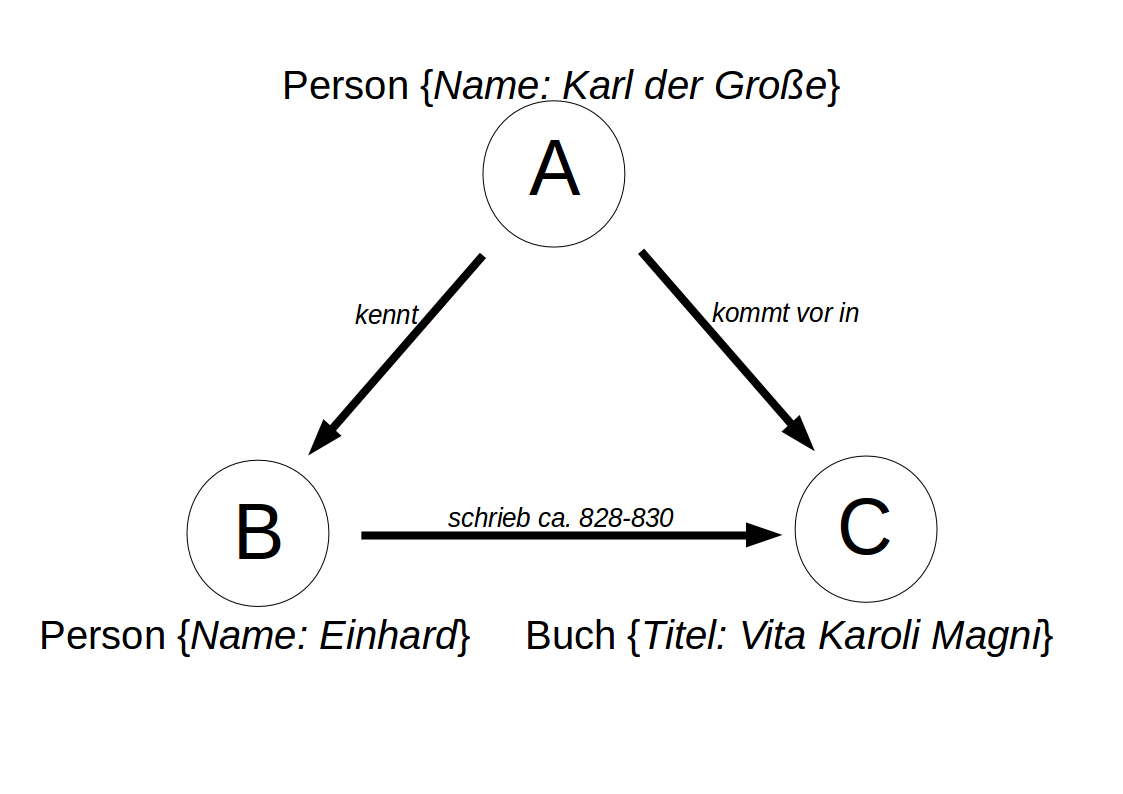
\includegraphics{Bilder/Beispielgraph.png}
\caption{Beispielgraph (Quelle: Kuczera)}
\label{beispielgraph}
\end{figure}

Der Beispielgraph zeigt oben einen Knoten (engl. Node) vom Typ (engl. Label) Person mit der Eigenschaft (engl. Property) Name. Diese hat den Wert ``Karl der Große''. Links unten ist ein weiter Knoten vom Typ Person mit dem Namen ``Einhard''. Rechts unten ist ein Knoten vom Typ Buch und dem Titel ``Vita Karoli Magni'' abgebildet. Die Kanten (engl. Edges) geben an, dass Karl der Große Einhard kannte, Einhard ca. 828-830 das Buch ``Vita Karoli Magni'' schrieb und Karl der Große in dem Buch vorkommt.

Knoten und Kanten können also noch zusätzliche Eigenschaften besitzen, in denen weitere Informationen gespeichert sind. Diese Eigenschaften sind spezifisch für die jeweiligen Knotentypen. So sieht man in der Abbildung, dass die beiden Knoten vom Typ Person jeweils noch die Eigenschaft Namen haben, deren Wert dann die Namen der Person angibt, während der Knoten vom Typ Buch die Eigenschaft Titel trägt, in dem der Titel des Buches abgespeichert wird.

Der wirkliche Mehrwert bei Graphdatenbanken ergibt sich aus gerichteten (also Verbinungen mit einer Richtung) und transitiven Beziehungen. Hat A eine direkte Kante zu B und B eine direkte Kante zu C dann ist A nicht direkt sondern transitiv mit C verbunden. Gerade wenn ein Graph sehr viele verschiedene solcher transitiven Verbindungen hat, lassen sich Muster und Verbindungen identifizieren, die in relationalen Modellen oft unentdeckt bleiben. Darüber hinaus bietet der Graph eine optimale Ausgangslage für anschließende Netzwerkanalyse des gesamten Graphen oder ausgewählter Subgraphen. War es in den digitalen Geisteswissenschaften bis vor einigen Jahren noch höchste Priorität überhaupt digitale Forschungsdaten bereitzustellen ist es heute die Herausforderung Daten in ihrem Kontext zu erfassen. Hierfür lassen sich Graphdatenbanken hervorragend nutzen.

\hypertarget{herkunft-und-idee}{%
\section{Herkunft und Idee}\label{herkunft-und-idee}}

Graphen gehen zurück auf die erste Hälfte des 18 Jahrhunderts. 1736 löste Leonhard Euler das ``Königsberger Brückenproblem'', das fragte ob es möglich sei, die 4 durch den Fluss getrennten Stadtbereiche, die über 7 Brücken verbunden waren jeweils einmal zu besuchen, ohne eine der Brücken zweimal zu nutzen (Abb. \ref{euler}).\footnote{Vgl. https://de.wikipedia.org/wiki/K\%C3\%B6nigsberger\_Br\%C3\%BCckenproblem.}

\begin{figure}
\centering
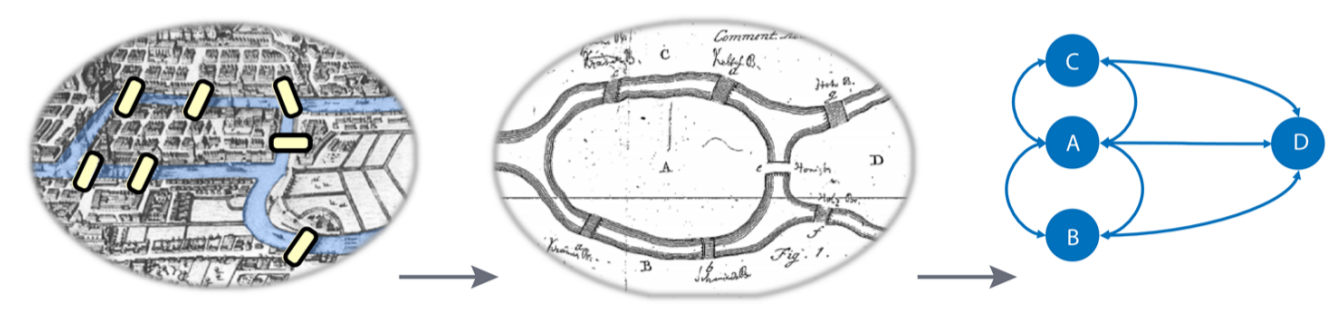
\includegraphics{Bilder/Eulersche-Bruecken.png}
\caption{Das Eulersche Brückenproblem (Needham/Hodler 2019, S. 2, Bild 1-1)}
\label{euler}
\end{figure}

Euler kam zu der Einsicht, dass nur die Verbindungen zwischen den 4 Bereichen der Stadt relevant sind und legte damit den Grundstein für die Graphtheorie und ihre Mathematik. Er zeigte, dass das Brückenproblem nicht lösbar war, da zu jedem Stadtbereich eine ungerade Anzahl von Brücken führte, es dürfe aber nur zwei Ufer mit einer ungeraden Anzahl geben.\footnote{Vgl. https://de.wikipedia.org/wiki/K\%C3\%B6nigsberger\_Br\%C3\%BCckenproblem.}

\hypertarget{graphtypen-und-strukturen}{%
\section{Graphtypen und Strukturen}\label{graphtypen-und-strukturen}}

\hypertarget{graph-und-nicht-graph}{%
\subsection{Graph und nicht Graph}\label{graph-und-nicht-graph}}

Auch wenn Graphen ihren Ursprung in der Mathematik haben so sind sie doch ein pragmatisches Werkzeug um Informationen zu modellieren und zu analysieren.

\begin{figure}
\centering
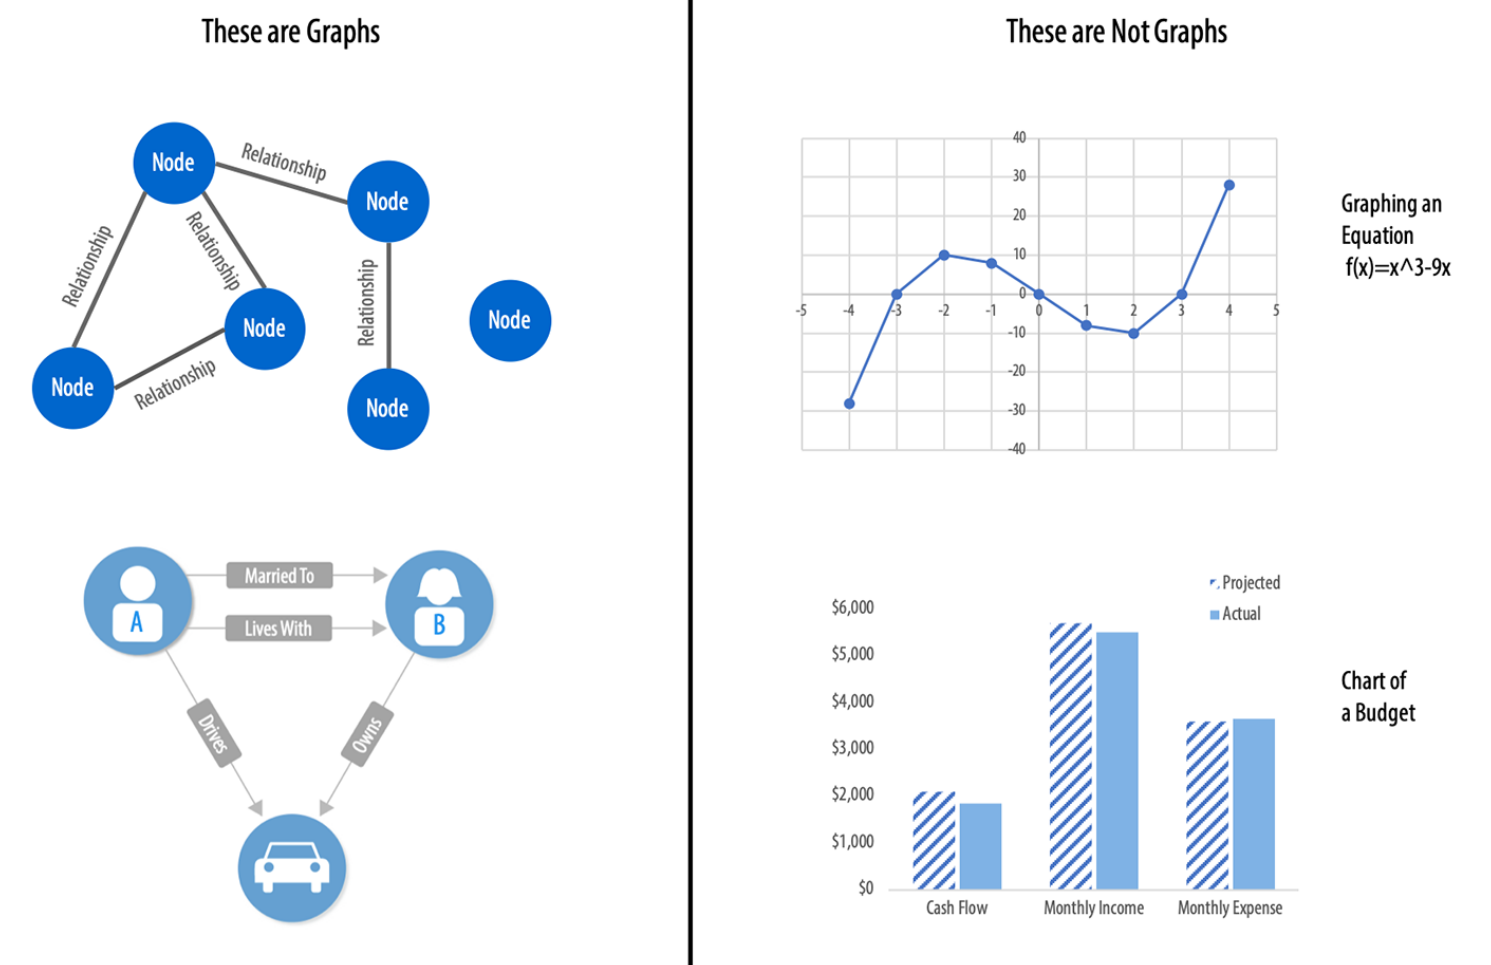
\includegraphics{Bilder/Graph-Algorithms/02-1-2-GraphsNotGraphs.png}
\caption{Graphen und nicht Graphen (Needham/Hodler 2019, S. 3, Bild 1-2)}
\label{graphnichtgraph}
\end{figure}

In diesem Reader geht es nicht um Graphen im Sinne von Lösung von Gleichungen wie in Abb. \ref{graphnichtgraph} rechts. Es geht um Informationen, die durch Knoten und Kanten dargestellt werden, wie links im Bild.

\hypertarget{labeled-property-graph}{%
\subsection{Labeled Property Graph}\label{labeled-property-graph}}

Einen Graphen, in dem die Knoten und Kanten Typen (Labels) und Eigenschaften (Properties) besitzen, nennt man ``Labeled Property Graph'' (LPG).

\begin{figure}
\centering
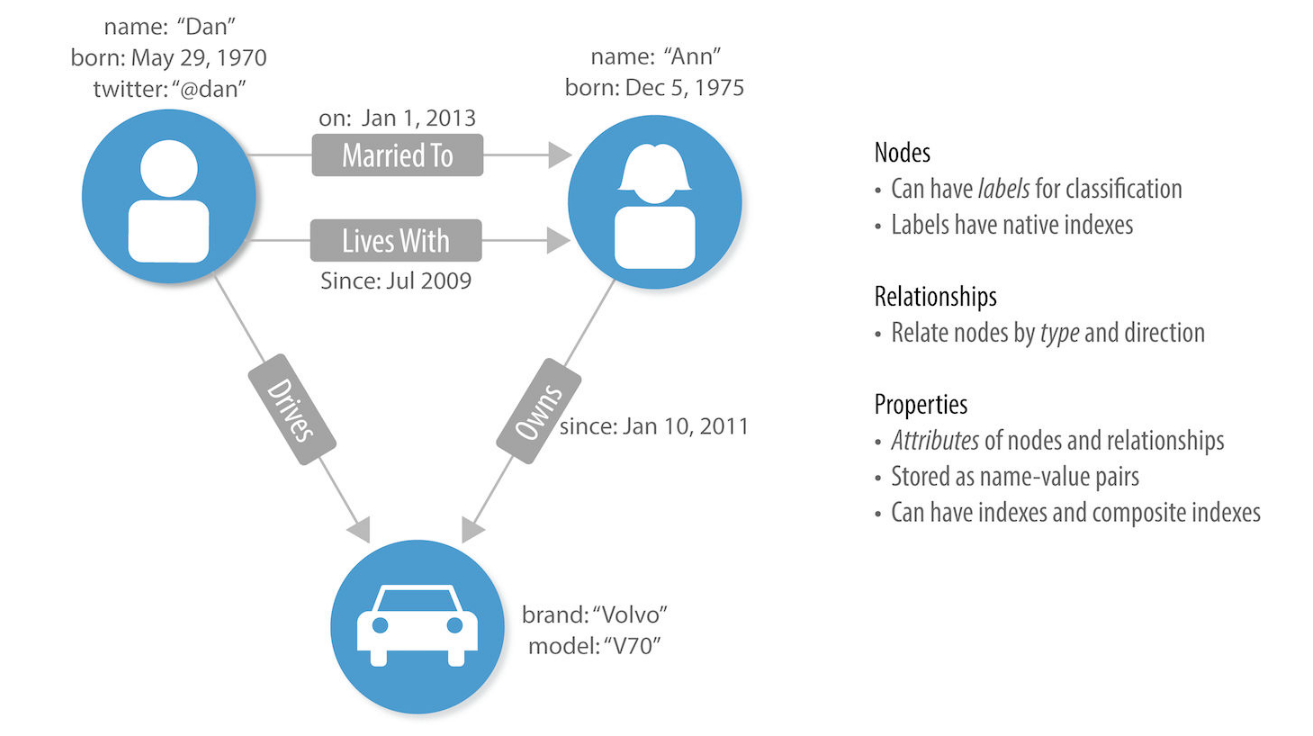
\includegraphics{Bilder/Graph-Algorithms/16-2-1-LabeledPropertyGraph.png}
\caption{Beispiel für einen Labeled-Property-Graphen (Needham/Hodler 2019, S. 16, Bild 2-1)}
\label{lpg}
\end{figure}

Der Graph in Abb. \ref{lpg} sagt beispielsweise aus, dass der Knoten links oben das Label ``männliche Person'' mit den zugehörigen Properties (name:`Dan', born etc.) trägt. Rechts daneben ist eine weibliche Person mit ihren Properties (name:`Ann', born: Dec 5, 1975) abgebildet. Die Kanten sagen aus, dass Ann am 1. Januar 2013 mit Dan zusammenlebte und seit Juli 2009 mit ihm verheiratet ist . Ann gehört gleichzeitig ein Auto (mit der Property Marke: `Volvo'), das von Dan gefahren wird. Hier werden in einfachen Schritten Informationen aus der ``realen Welt'' abgebildet. In den nächsten Abschnitten geht es nun um die Konzepte dahinter.

\hypertarget{einfache-graphtypen}{%
\subsection{Einfache Graphtypen}\label{einfache-graphtypen}}

In Abb. \ref{einfachegraphtypen} sind verschiedene Graphtypen abgebildet. Im Beispiel links ist ein einfacher Graph dargestellt, in dem jedes Knotenpaar nur eine Verbindung haben kann.

\begin{figure}
\centering
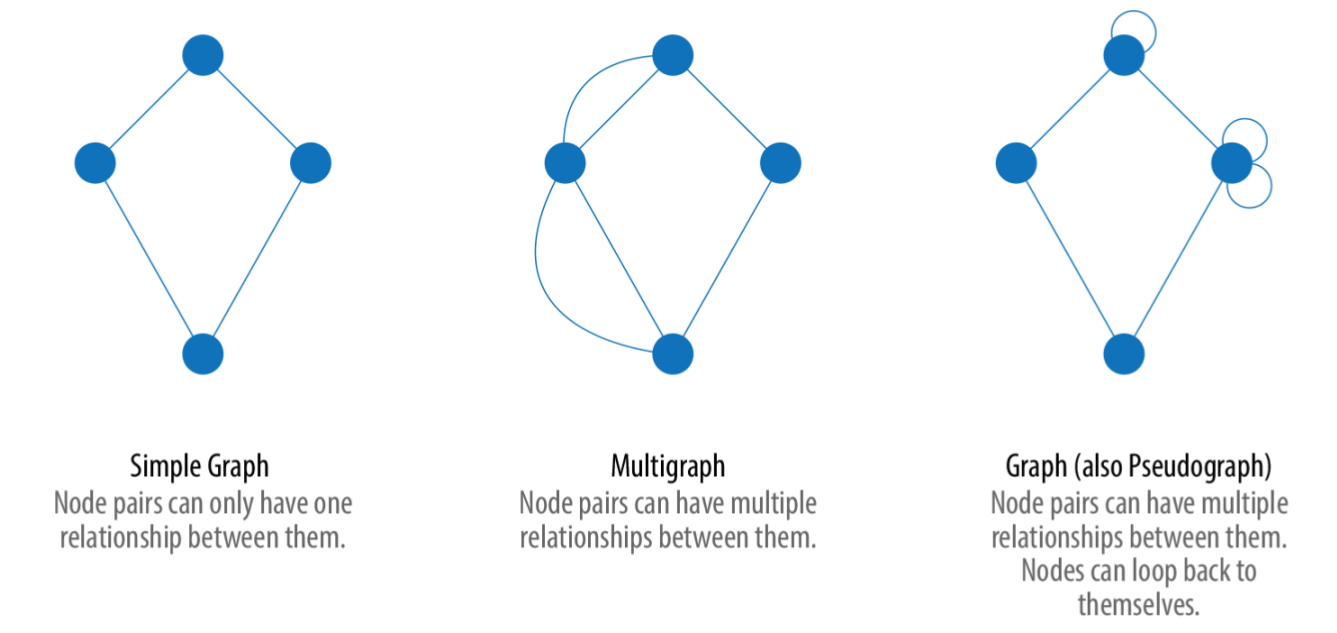
\includegraphics{Bilder/Graph-Algorithms/17-2-2-TypesOfGraphs.png}
\caption{Einfache Graphtypen (Needham/Hodler 2019, S. 17, Bild 2-2)}
\label{einfachegraphtypen}
\end{figure}

Im mittleren Beispiel sind mehrere Verbindungen zwischen Knotenpaaren möglich. Das rechte Beispiel ergänzt sich noch um die Möglichkeit, Verbindungen von Knoten wieder zu ihnen selbst zurück zu ermöglichen.

Die untere Bildhälfte zeigt links ein Beispiel für einen zufälligen Graphen, aus dem sich keine hierarchischen oder strukturellen Informationen ablesen lassen. 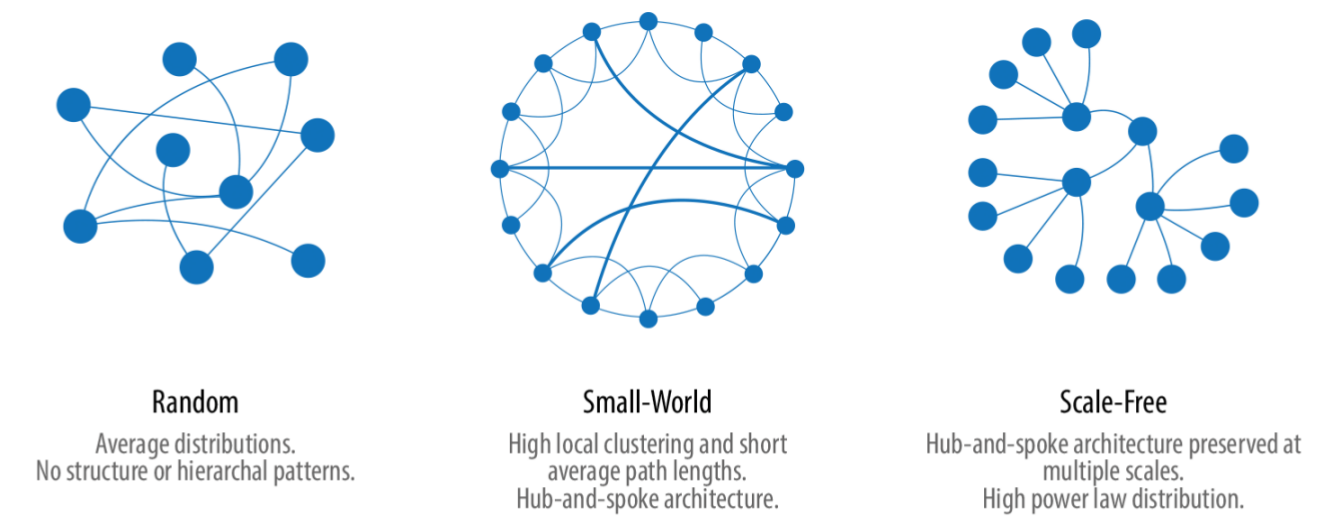
\includegraphics{Bilder/Graph-Algorithms/17-2-3-RandomSmallWorldScaleFree.png}

In der Mitte ist ein Small-World-Graph abgebildet, der lokal stark geclustert ist und eine geringe durchschnittliche Pfadlänge hat. Die rechte Abbildung zeigt ein skalenfreies Netzwerk, wie beispielsweise das World-Wide-Web.

In Tab. \ref{tab:charaktertyp} werden charakteristische Möglichkeiten zur Typisierung von Graphen gegenübergestellt.

\begin{longtable}[]{@{}lll@{}}
\toprule
\begin{minipage}[b]{0.22\columnwidth}\raggedright
Graphattribute\strut
\end{minipage} & \begin{minipage}[b]{0.26\columnwidth}\raggedright
Unterschiede\strut
\end{minipage} & \begin{minipage}[b]{0.44\columnwidth}\raggedright
Überlegungen zum Algorithms\strut
\end{minipage}\tabularnewline
\midrule
\endhead
\begin{minipage}[t]{0.22\columnwidth}\raggedright
Verbundene und nichtverbundene Graphen\strut
\end{minipage} & \begin{minipage}[t]{0.26\columnwidth}\raggedright
Gibt es einen Pfad (Länge egal) zwischen zwei beliebigen Knoten eines Graphen\strut
\end{minipage} & \begin{minipage}[t]{0.44\columnwidth}\raggedright
Knoteninseln können zu unvorhergesehenem Verhalten, wie Abbruch oder Auslassen von Knoteninseln führen\strut
\end{minipage}\tabularnewline
\begin{minipage}[t]{0.22\columnwidth}\raggedright
Gewichtete und ungewichtete Graphen\strut
\end{minipage} & \begin{minipage}[t]{0.26\columnwidth}\raggedright
Gibt es (domänen-spezifische) Werte für Wichtungen an Knoten und Kanten\strut
\end{minipage} & \begin{minipage}[t]{0.44\columnwidth}\raggedright
Werte machen den Graphen reicher an Informationen; Viele Algoritmen benötigen gewichtende Werte\strut
\end{minipage}\tabularnewline
\begin{minipage}[t]{0.22\columnwidth}\raggedright
Gerichtete und ungerichtete Graphen\strut
\end{minipage} & \begin{minipage}[t]{0.26\columnwidth}\raggedright
Ist eine Verbindung hierarchisch oder gegenseitig\strut
\end{minipage} & \begin{minipage}[t]{0.44\columnwidth}\raggedright
Die Richtung einer Kante sind für viele Auswertungen von Relevanz\strut
\end{minipage}\tabularnewline
\begin{minipage}[t]{0.22\columnwidth}\raggedright
Zyklische und nicht zyklische Graphen\strut
\end{minipage} & \begin{minipage}[t]{0.26\columnwidth}\raggedright
In zyklischen Graphen können Pfade können wieder zum Startknoten zurückkehren\strut
\end{minipage} & \begin{minipage}[t]{0.44\columnwidth}\raggedright
Zyklische Graphen sind weit verbreitet. Bei der Auswertung mit Graphalgorithmen muss der Graph aber möglicherweise bearbeitet werden\strut
\end{minipage}\tabularnewline
\begin{minipage}[t]{0.22\columnwidth}\raggedright
Graphdichte\strut
\end{minipage} & \begin{minipage}[t]{0.26\columnwidth}\raggedright
Das Verhältnis von Kanten zu Knotenzahl\strut
\end{minipage} & \begin{minipage}[t]{0.44\columnwidth}\raggedright
Extrem dichte oder extrem dünne Graphen können die Analyse erschweren. Ggf. können Änderungen an der Modellierung helfen, sofern es die Domäne zulässt\strut
\end{minipage}\tabularnewline
\begin{minipage}[t]{0.22\columnwidth}\raggedright
Monopartite, bipartite, und k-partite Graphen\strut
\end{minipage} & \begin{minipage}[t]{0.26\columnwidth}\raggedright
Gibt es einen, zwei oder mehrere Knotentypen\strut
\end{minipage} & \begin{minipage}[t]{0.44\columnwidth}\raggedright
Mehr Knotentypen erleichtern in den Geisteswissenschaften die Modellierung, Graphalgorithmen arbeiten oft aber nur mit einem Knotentyp\strut
\end{minipage}\tabularnewline
\bottomrule
\label{tab:charaktertyp}
\end{longtable}

Quelle: \href{Needham/Hodler\%202019}{https://www.oreilly.com/library/view/graph-algorithms/9781492047674/}, S. 18-19.

\hypertarget{verbundene-und-nichtverbundene-graphen}{%
\subsection{Verbundene und nichtverbundene Graphen}\label{verbundene-und-nichtverbundene-graphen}}

Sind in einem Graphen mehrere Gruppen von verbundenen Knoten vorhanden und es gibt zwischen den Gruppen keine Verbindungen, handelt es sich um nichtverbundene Graphen.

\begin{figure}
\centering
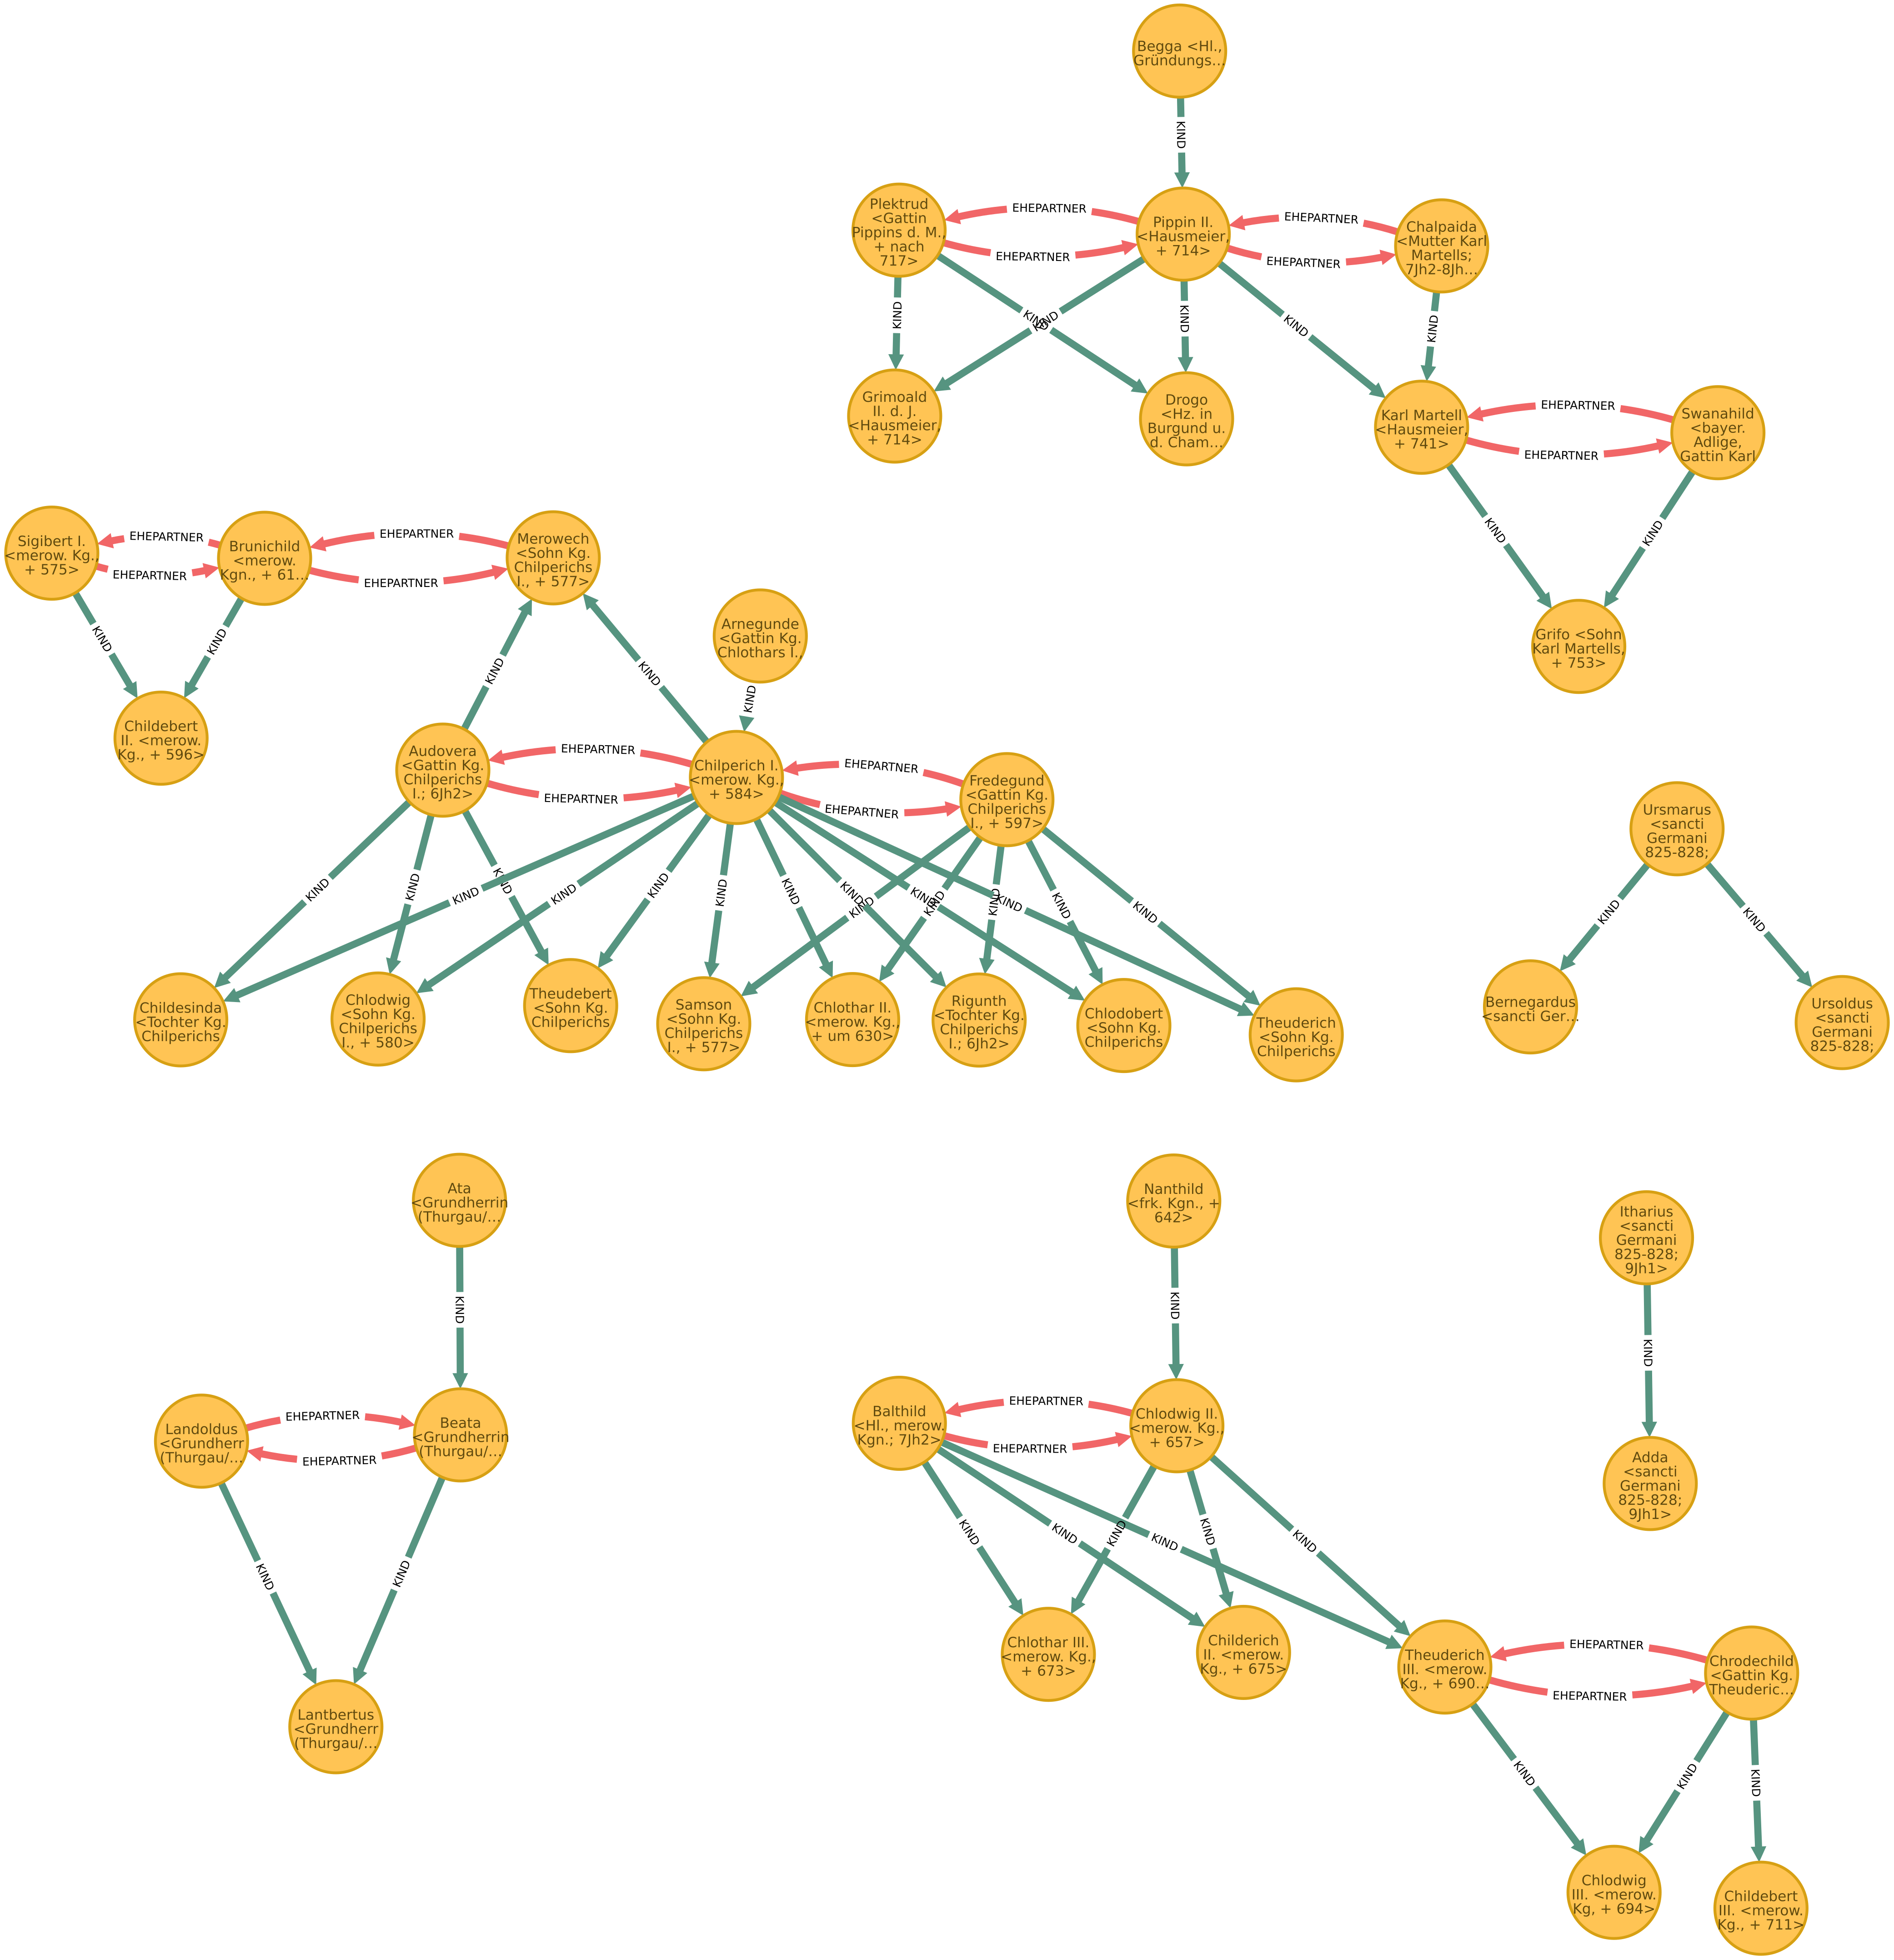
\includegraphics{Bilder/disconnectedGraph.png}
\caption{Nichtverbundener Graph (Quelle: Kuczera)}
\label{nichtverbundener}
\end{figure}

Das Beispiel in Abb. \ref{nichtverbundener} zeigt einen Graphen mit Personen und ihren Verwandtschaftsbeziehungen. Es gibt mehrere Stammbäume, die nicht miteinander verbunden sind.

Abb. \ref{verbundener} zeigt einen verbundenen Graphen, bei dem alle Knoten mindestens eine Kante haben und jeder Knoten jeden anderen über einen Pfad erreichen kann. Hier wird ein Ausschnitt aus einer Graphdatenbank gezeigt, in die eine XML-Text-Datei als XML-Baum importiert wurde. Da es sich bei jeder XML-Datei um einen Baum handelt und jeder XML-Knoten Teil dieses Baumes ist, gibt es keine nichtverbundenen Teile.

\begin{figure}
\centering
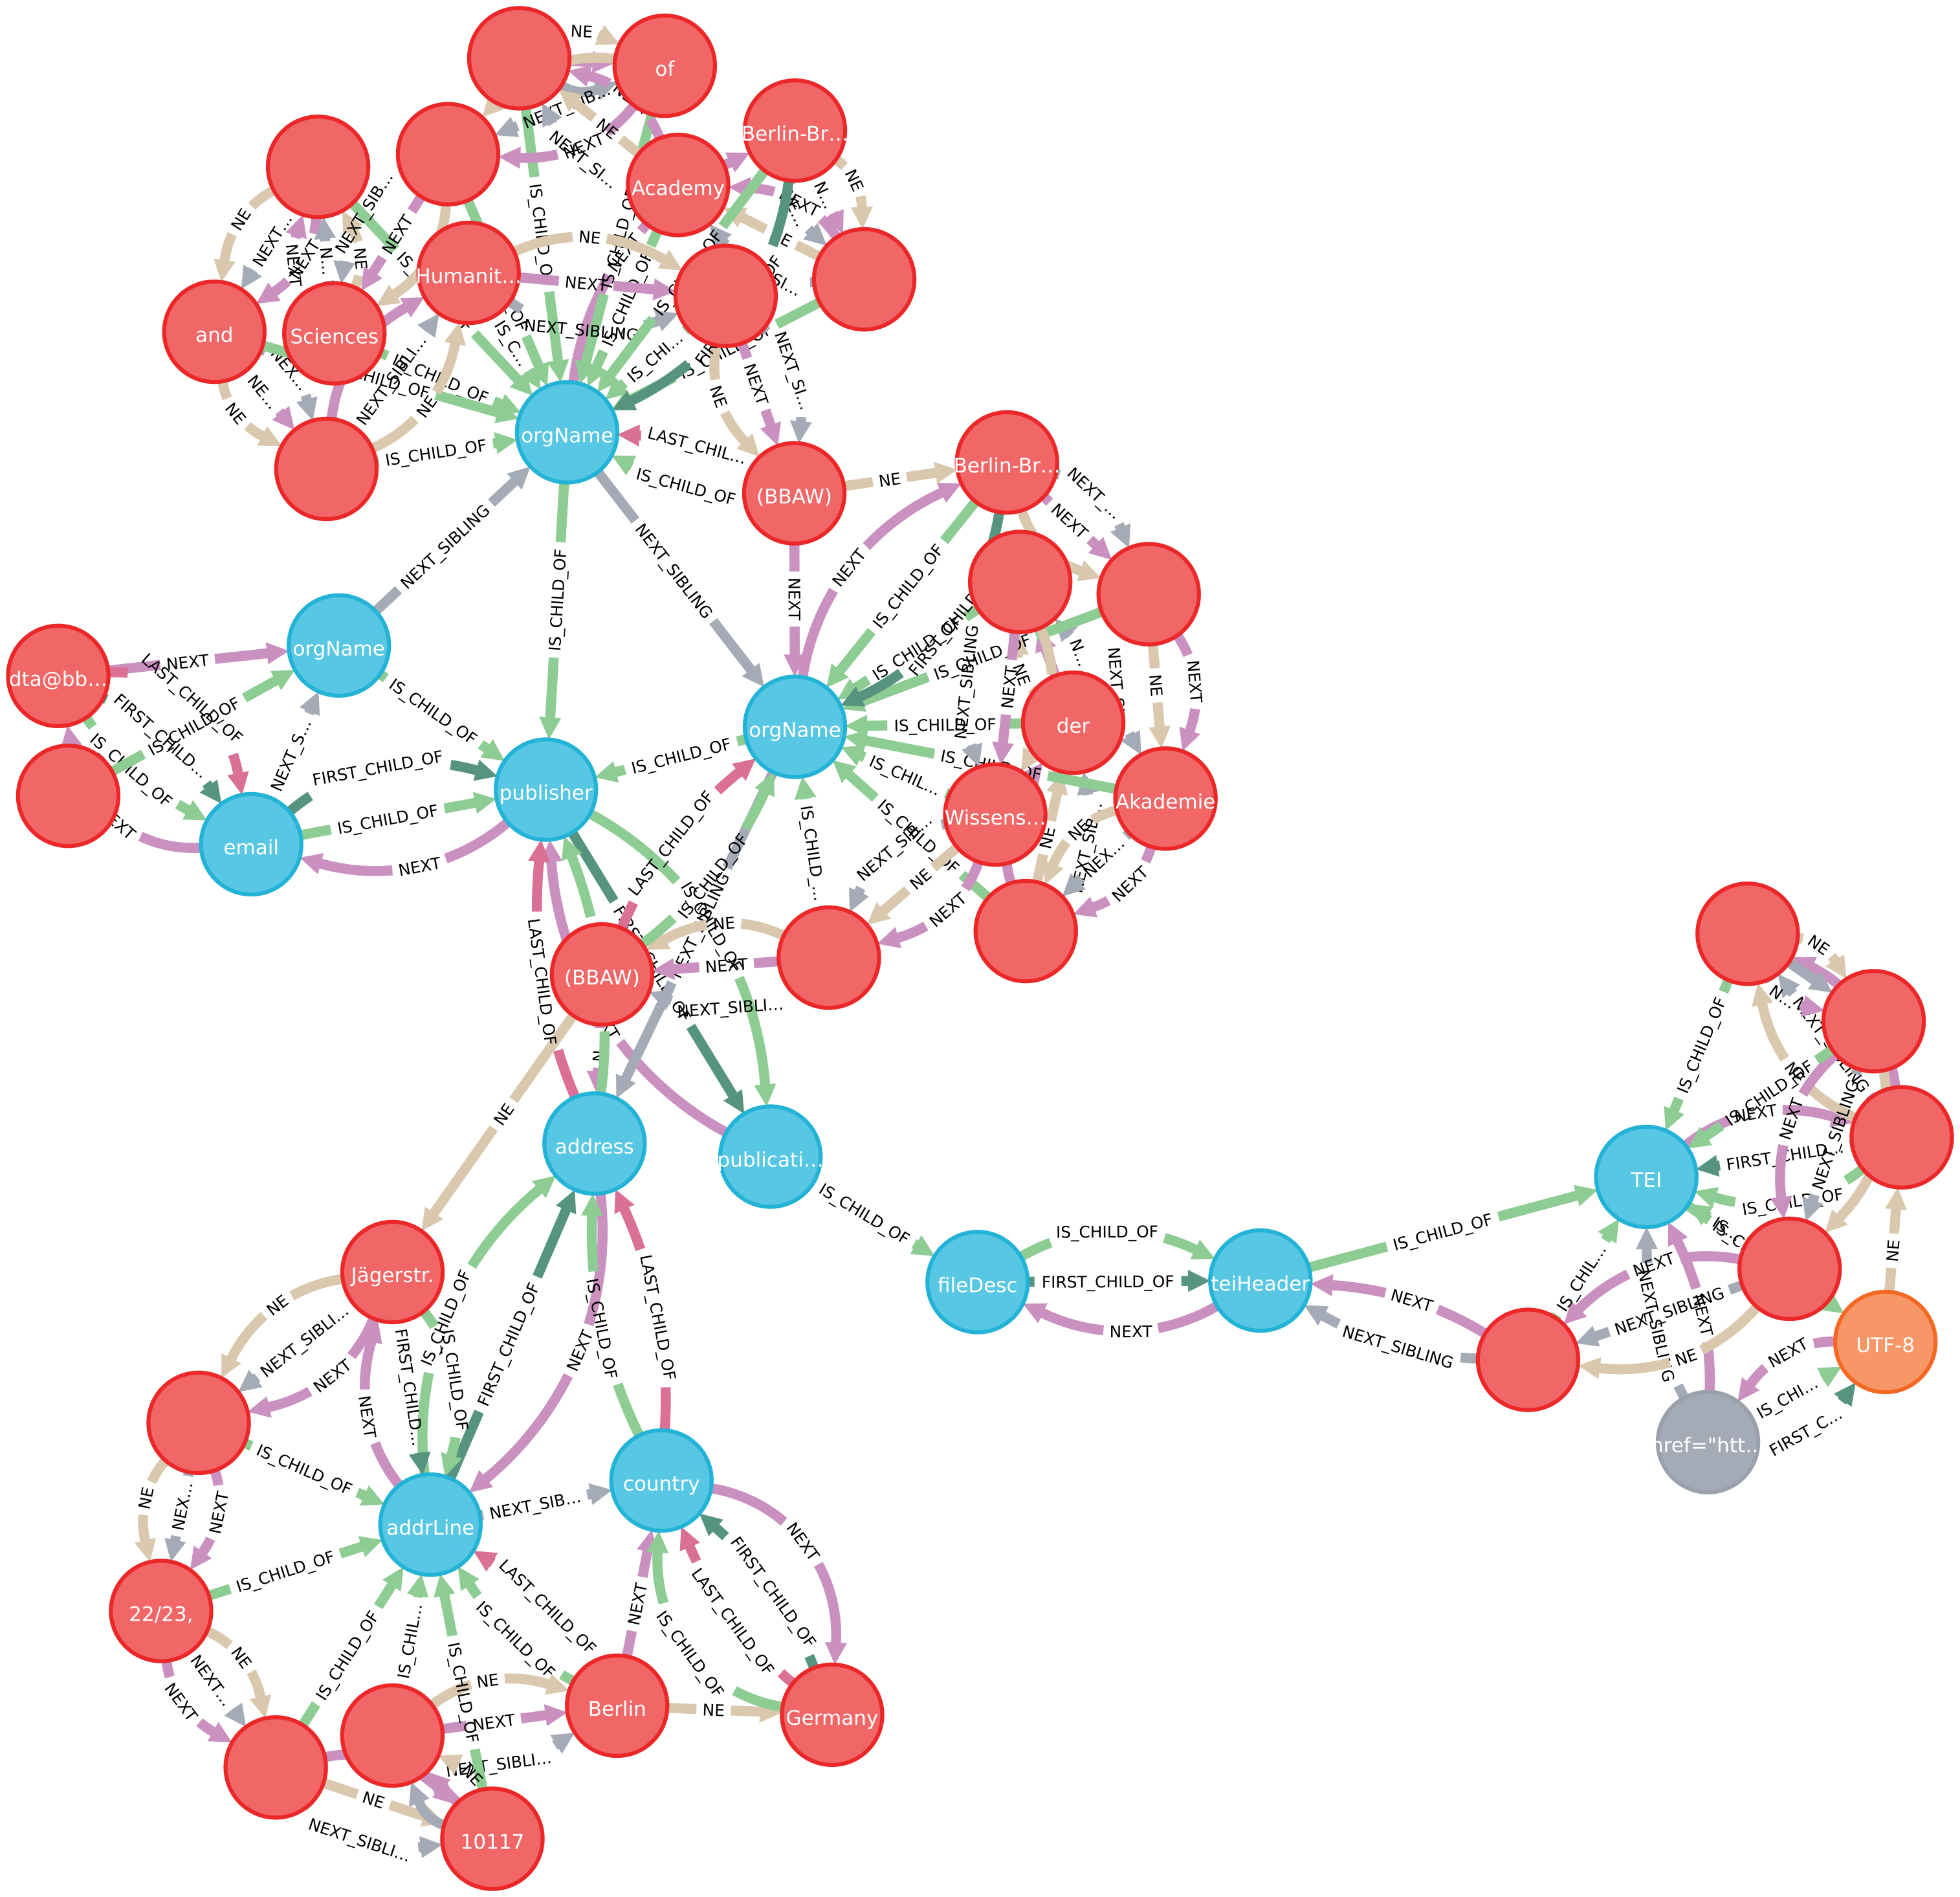
\includegraphics{Bilder/connectedGraph.png}
\caption{Verbundener Graph (Quelle: Kuczera)}
\label{verbundener}
\end{figure}


\hypertarget{gewichtete-und-ungewichtete-graphen}{%
\subsection{Gewichtete und ungewichtete Graphen}\label{gewichtete-und-ungewichtete-graphen}}

In ungewichteten Graphen besitzen die Kanten keinen Wert zu Gewichtung.

\begin{figure}
\centering
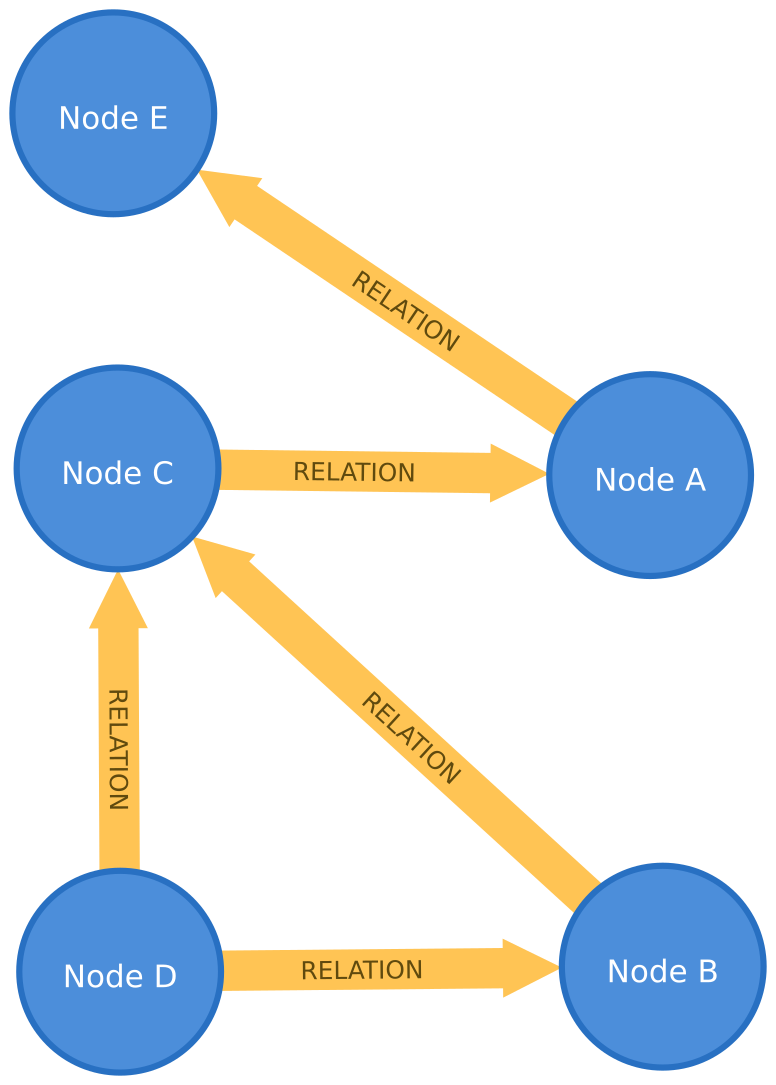
\includegraphics{Bilder/unWeightedGraph.png}
\caption{Ungewichteter Graph (Quelle: Kuczera)} 
\label{ungewichteter}
\end{figure}

Im Graphen in Abb. \ref{ungewichteter} werden Beziehungen zwischen Personen abgebildet. Über die Intensität der Beziehungen wird nichts gesagt. In  Abb. \ref{gewichteter} wurde den Beziehungen jeweils ein Wert zwischen 0 und 100 zugeordnet.

\begin{figure}
\centering
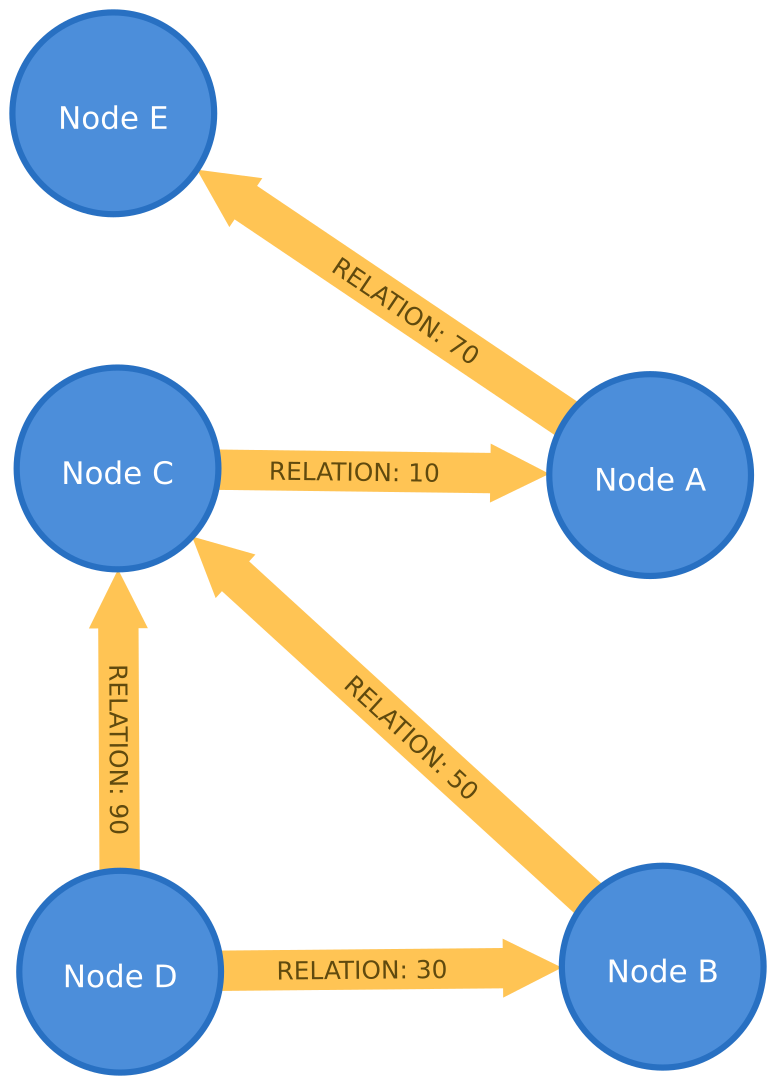
\includegraphics{Bilder/weightedGraph.png}
\caption{Gewichteter Graph (Quelle: Kuczera)}
\label{gewichteter}
\end{figure}

Werden solche Angaben ergänzt, werden die Informationen im Graph wertvoller. Werte für Wichtungen können beispielsweise Entfernungen, Kosten, Kapazitäten oder auch domänenspezifische Priorisierungen sein.

\hypertarget{gerichtete-und-ungerichtete-graphen}{%
\subsection{Gerichtete und ungerichtete Graphen}\label{gerichtete-und-ungerichtete-graphen}}

In einem ungerichteten Graphen geht eine Beziehungen immer in beide Richtungen (beispielsweise EHEPARTNER\_VON). In einem gerichteten Graphen haben Beziehungen eine Richtung. Betrachtet man einen Knoten, gibt es eingehende Kanten, die auf den Knoten zeigen und ausgehende Kanten, die von dem Knoten ausgehen. Mit der Angabe von Richtung wird eine zusätzliche Informationsdimension hinzugefügt. Angenommen im linken Beispiel der Abb. \ref{gerichteteundungerichtete} würden die Knoten Personen und die ungerichtete Kante ihre gegenseitige Freundschaft darstellen. Daraus ergibt sich, dass Person A mit Person B befreundet ist.

\begin{figure}
\centering
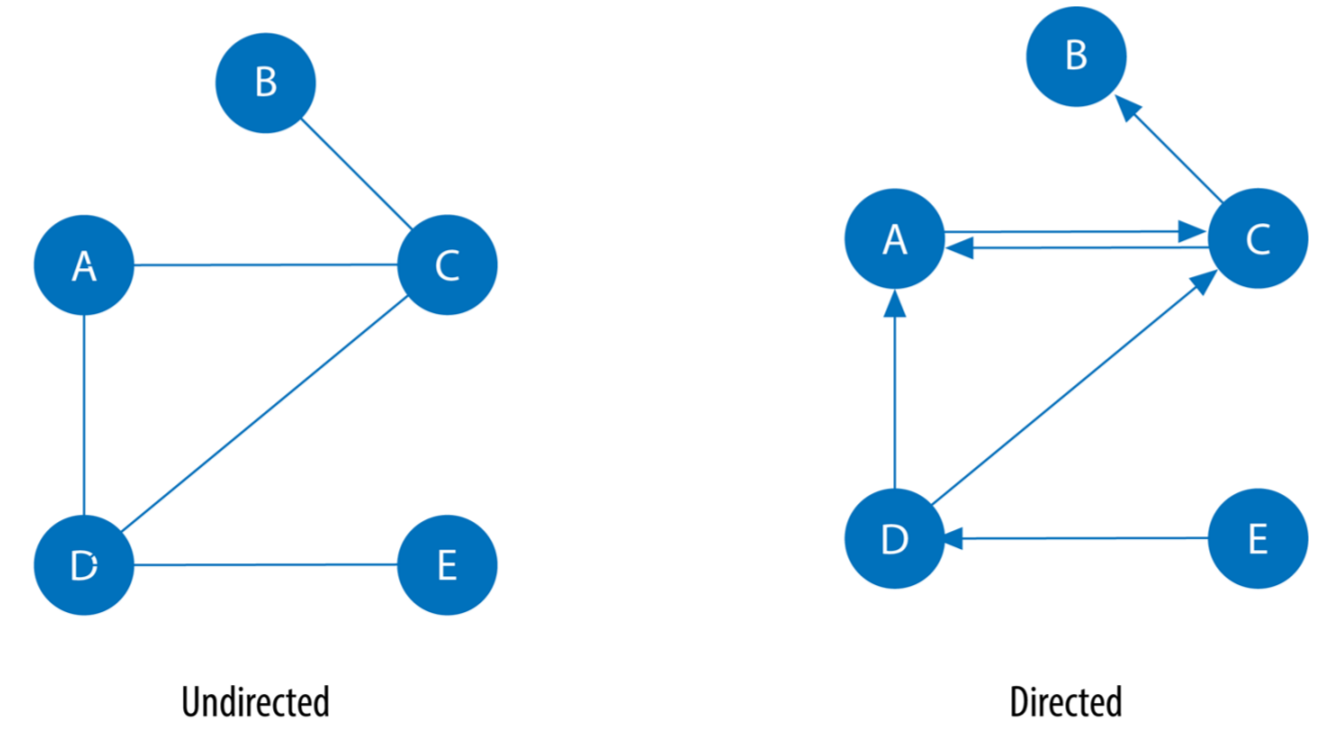
\includegraphics{Bilder/Graph-Algorithms/21-2-7-UnDirected.png}
\caption{Gerichtete und ungerichtete Graphen (Needham/Hodler 2019, S. 21, Bild 2-7)}
\label{gerichteteundungerichtete}
\end{figure}

Erweitern wir das Beispiel für die rechte Abbildung, so dass die Freundschafts-Kanten gerichtet sind, so wird es möglich, zu zeigen, dass Person D für Person A freundschaftliche Gefühle hegt, die A aber nicht erwidert. Nehmen wir noch eine Wichtung der Freundschafskanten hinzu, könnte man modellieren, dass die freundschaftlichen Gefühle von Person C gegenüber A mit 0,8 gewichtet sind, umgekehrt die Zuneigung von Person A zu Person C aber nur mit 0,3.

Auch bei der Modellierung von Verwandtschaft kommen gerichtete und ungerichtete Verbindungen vor.

\begin{figure}
\centering
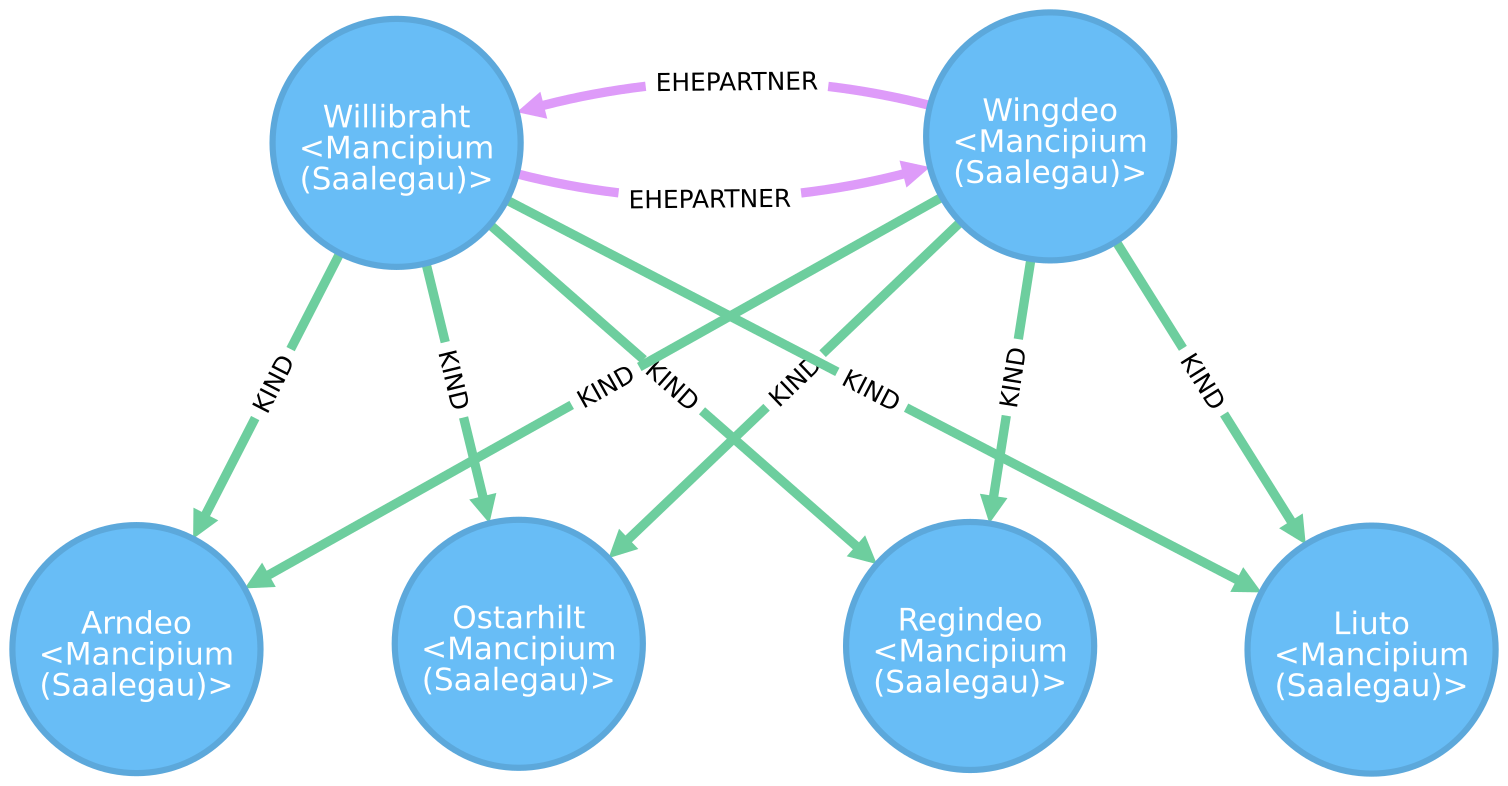
\includegraphics{Bilder/NomenEtGensBeispiel1.png}
\caption{Verwandtschaft im Graphen mit gerichteten und ungerichteten Kanten (Quelle: Kuczera)}
\label{nomenetgensbeispiel}
\end{figure}

In der Graphdatenbank neo4j müssen Kanten eine Richtung haben. Ungerichtete Beziehungen kann man mit zwei Kanten vom gleichen Typ aber unterschiedlicher Richtung zwischen einem Knotenpaar modellieren. Im Verwandtschaftsbeispiel Abb. \ref{nomenetgensbeispiel} sind die zwei Personenknoten der Eltern mit zwei EHEPARTNER-Kanten unterschiedlicher Richtung verbunden. Es handelt sich um eine ungerichtete Beziehung, da es rechtlich nicht möglich ist, dass eine Person mit einer anderen Person verheiratet ist, umgekehrt aber nicht. Für die Eltern-Kind-Beziehung reicht eine Kante, da diese Beziehung hierarchisch ist.

\hypertarget{installation-und-start}{%
\section{Installation und Start}\label{installation-und-start}}

Informationen zur Installation von neo4j finden Sie auf den Dokumentationsseiten unter \url{https://neo4j.com/docs/operations-manual/current/installation/}. Für den normalen Nutzer empfiehlt sich die Installation von \href{https://neo4j.com/download/}{neo4j-Desktop}. Unter \url{https://neo4j.com/blog/this-week-in-neo4j-getting-started-with-neo4j-desktop-and-browser-graphileon-personal-edition-intuitive-detections-research-with-neo4j/?ref=twitter\#features-1} finden sich Videos, in denen die Installation von \href{https://www.youtube.com/watch?v=8yWhuUnPapw}{neo4j-Desktop} und erste Schritte im \href{https://www.youtube.com/watch?v=rQTximyaETA}{neo4j-Browser} erklärt werden.

\hypertarget{zusammenfassung}{%
\section{Zusammenfassung}\label{zusammenfassung}}

In diesem Kapitel wurde kurz auf die Ursprünge von Graphen eingegangen und verschiedene Typen von Graphen vorgestellt. Festzuhalten ist, dass es sich in den Digitalen Geisteswissenschaften in der Regel um Mischformen der vorgestellen Graphtypen handelt. Je nach Domäne werden Graphen hoher Dichte, mit vielen Knotentypen oder auch hierarchischen Strukturen benötigt. Modelle in den Digitalen Geisteswissenschaften haben meist mehrere Knotentypen und viele Kantentypen. Dies macht wiederum die direkte Anwendung von Graph-Algorithmen schwierig, so dass Graph-Transformationen notwendig werden können.

\hypertarget{das-projekt-regesta-imperii-oder-wie-suchen-onlinenutzer-regesten}{%
\chapter{Das Projekt Regesta Imperii oder ``Wie suchen Onlinenutzer Regesten?''}\label{das-projekt-regesta-imperii-oder-wie-suchen-onlinenutzer-regesten}}

\hypertarget{das-projekt-regesta-imperii}{%
\section{Das Projekt Regesta Imperii}\label{das-projekt-regesta-imperii}}

Das Projekt Regesta Imperii wurde von Johann-Friedrich Böhmer im Jahr 1829 begonnen. Ursprünglich als Vorarbeit zu den \href{https://www.mgh.de}{Monumenta Germaniae Historica} angelegt, wurde es mit einem erweiterten Regestenkonzept bald zu einem unverzichtbaren Grundlagenwerk. In den Regesta Imperii werden Inhaltsangaben von Urkunden erstellt, die rechtlich relevante Personen, Inhalte, Orte und Sachverhalte in deutscher Sprache zusammenfassen. Zeitlich umfassen sie den Rahmen von den \href{https://de.wikipedia.org/wiki/Karolinger}{Karolingern} (7. Jahrhundert) bis Kaiser \href{https://de.wikipedia.org/wiki/Maximilian_I._(HRR)}{Maximilian} (gestorben 1519).

\begin{figure}
\centering
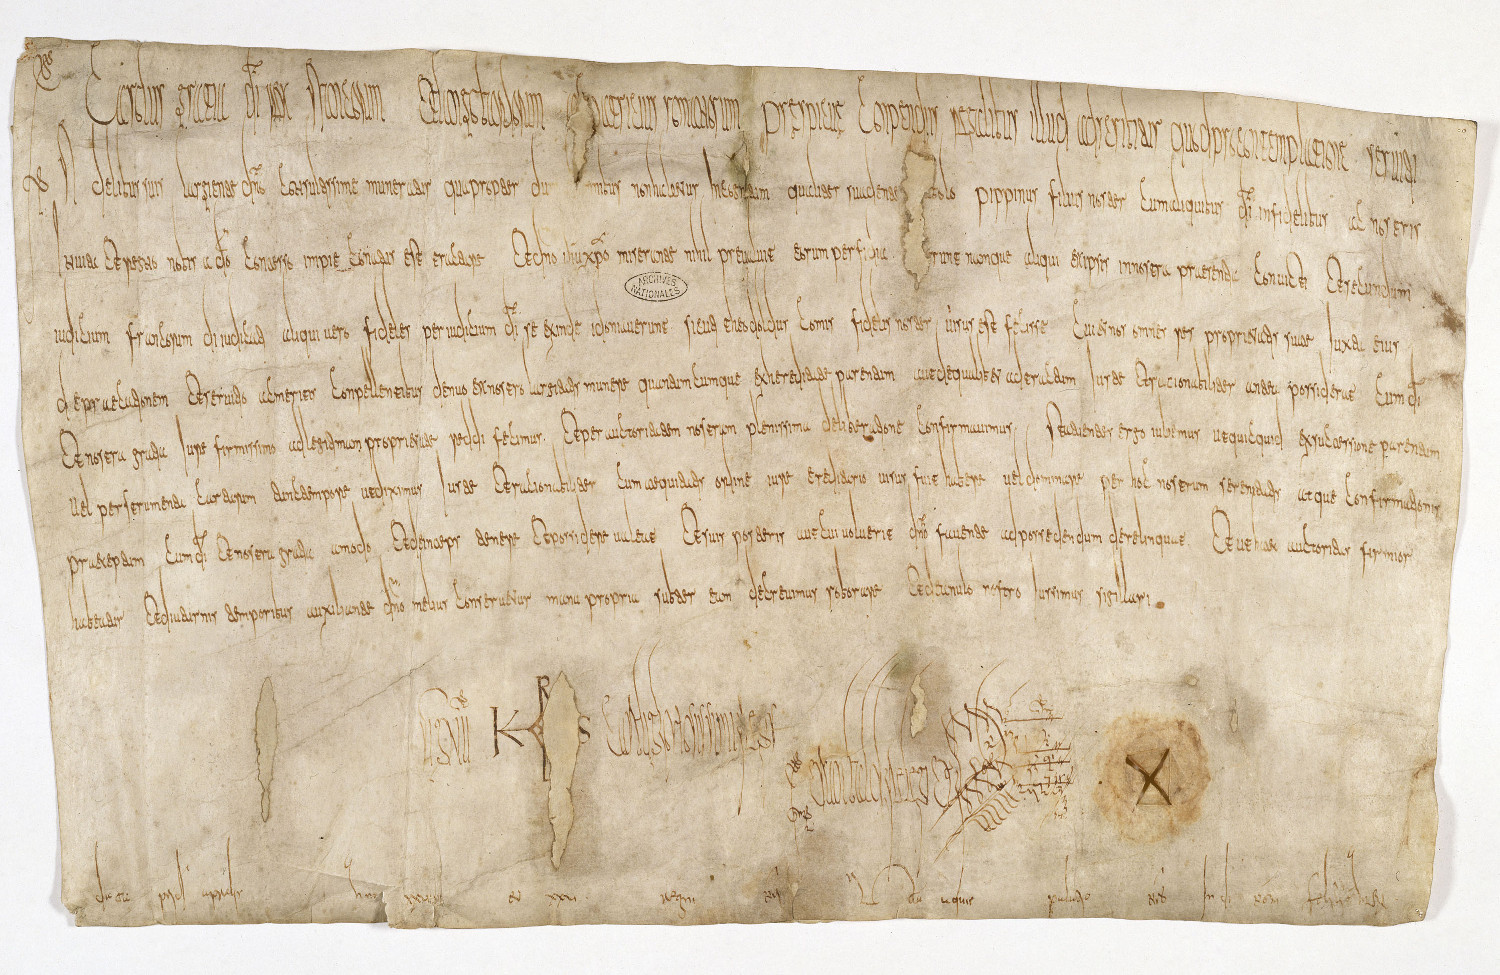
\includegraphics{Bilder/Beispielurkunde.jpg}
\caption{Urkunde zum Regest RI I n. 336, in: Regesta Imperii Online. URL: http://www.mgh.de/bibliothek/virtueller-lesesaal/ddkar/01/?p=XXXI}
\label{urkunde}
\end{figure}

Ursprünglich von der DFG gefördert, sind die Regesta Imperii heute Teil des Bund-Ländergeförderten Akademienprogramms und werden von der Akademie der Wissenschaften und der Literatur, Mainz, der Berlin-Brandenburgischen Akademie der Wissenschaften und der Akademie der Wissenschaften, Wien betreut.

Die Regesta Imperii arbeiten vor allem herrscherzentriert, d.h. in den Regesten muss der Herrscher eine zentrale Rolle spielen. Bei Urkundenregesten hat er selbst die Urkunde ausgestellt, bei historiographischen Regesten werden den Herrscher betreffende historische Hintergründe zusammengefasst.

\begin{figure}
\centering
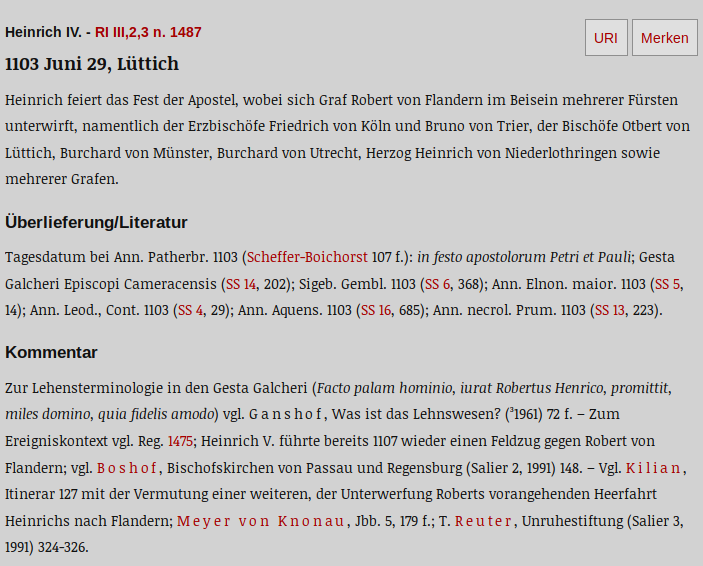
\includegraphics{Bilder/RI2Graph/ReggH4-Nr-1487.png}
\caption{RI III,2,3 n. 1487, in: Regesta Imperii Online, URI: http://www.regesta-imperii.de/id/cf75356b-bd0d-4a67-8aeb-3ae27d1dcefa.}
\label{regest}
\end{figure}

In der Kopfzeile des Regests in Abb. \ref{regest} werden der Herrscher sowie Abteilung, Band und Regestennummer genannt. Die darunterliegende Datierungszeile nennt das Ausstellungsdatum der Urkunden und den Handlungs- bzw. Ausstellungsort. Es folgt der Regestentext mit der Zusammenfassung der Urkunde, Hinweise zur Originaldatierung, die Kanzleivermerke und schließlich Angaben zur Überlieferungssituation (Gibt es eine Originalurkunde, wo liegt sie, gibt es ggf. Abschriften etc.).

\hypertarget{die-digitalisierung-der-regesta-imperii}{%
\section{Die Digitalisierung der Regesta Imperii}\label{die-digitalisierung-der-regesta-imperii}}

Im Rahmen eines von der DFG geförderten Projekts wurden die Regesta Imperii gemeinsame von der Akademie der Wissenschaften, Mainz und der Bayrischen Staatsbibliothek München von 2001 bis 2006 komplett digitalisiert. Alle seit 2006 erschienenen Regesten wurden sofort im Volltext online gestellt. Glücklicherweise hatte die Mainzer Akademie die Rechte selbst inne, so dass der Veröffentlichung als Volltext im Internet keine rechtlichen Hürden im Wege standen. Rückblickend lässt sich feststellen, dass der Absatz der gedruckten Bände nicht gelitten sondern teilweise sogar etwas zugelegt hat.

\hypertarget{wie-suchen-online-nutzer-regesten}{%
\section{Wie suchen Online-Nutzer Regesten ?}\label{wie-suchen-online-nutzer-regesten}}

Ende 2013 wurde das Suchverhalten der Nutzer der Online-Regestensuche im Rahmen eines Vortrages auf der Digital-Diplomatics-Konferenz in Paris in den Blick genommen.\footnote{Vgl. Kuczera, Andreas; Schrade, Torsten: From Charter Data to Charter Presentation: Thinking about Web Usability in the Regesta Imperii Online. Vortrag auf der Tagung ›Digital Diplomatics 2013 -- What ist Diplomatics in the Digital Environment?‹ Folien: https://prezi.com/vvacmdndthqg/from-charta-data-to-charta-presentation/.} Ein interessantes Ergebnis war die Häufigkeitsverteilung der Treffermengen pro Suchanfrage.

\begin{figure}
\centering
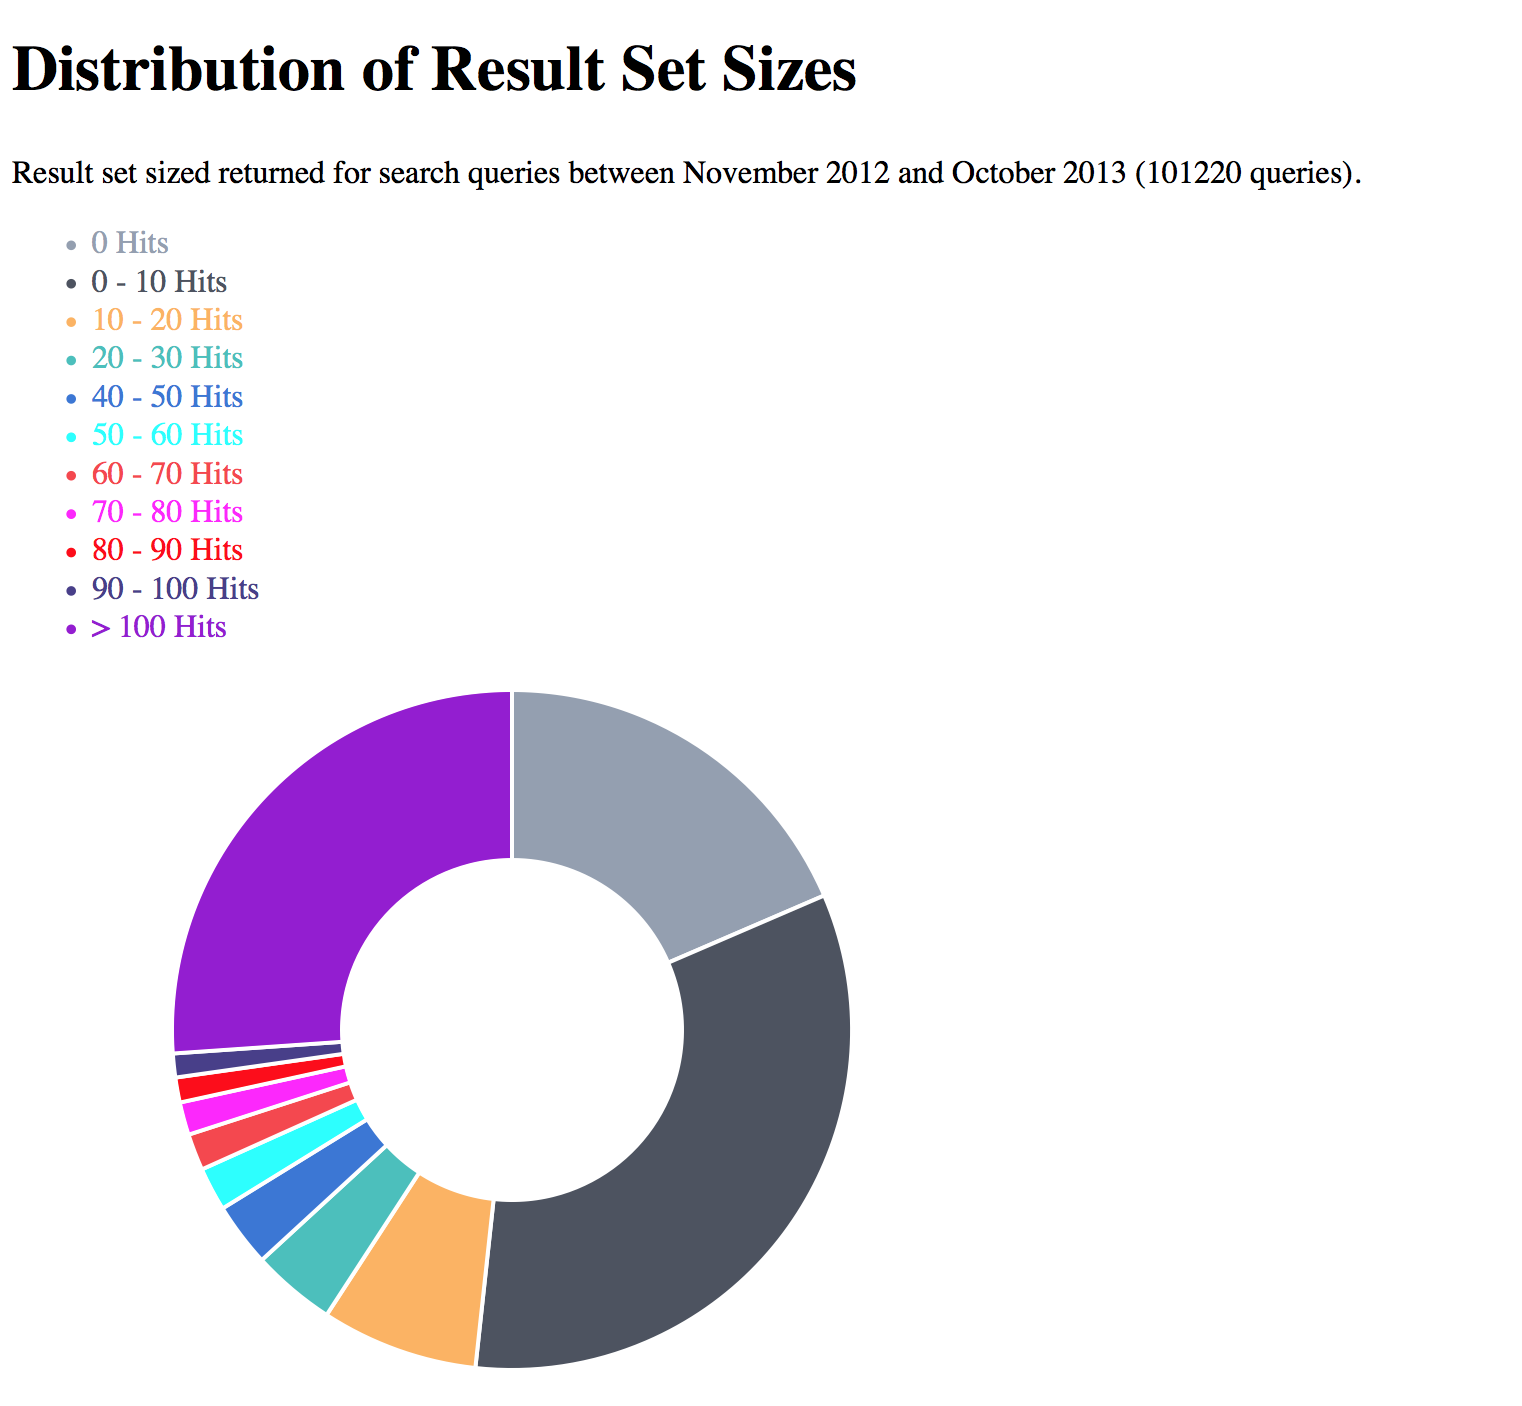
\includegraphics{Bilder/2012-Nutzungsformen_der_RI.png}
\caption{Treffermengen pro Suchanfragen im Jahr 2013.}
\label{treffermengen}
\end{figure}

In Abb. \ref{treffermengen} ist die Treffermenge in Zehnerschritten angegeben. Die hellgraue Gruppe oben rechts hat keine Treffer, die dunkelgraue Gruppe einen bis zehn Treffer, die gelbe Gruppe 11 bis 20 usw. Die lila Gruppe hat mehr als hundert Treffer. Überraschend war die große Gruppe mit über 100 Treffern. Hinzu kam, dass über 68\% der Nutzer nur ein Suchwort in die Suchmaske eingegeben haben, wobei das beliebteste Suchwort \emph{Heinrich} Ende 2013 zu über 18.000 Treffern führte. Auf der Ergebnisseite hieß es dann: ``Sie suchten nach \emph{Heinrich}. Ihre Suche erzielte 18884 Treffer {[}\ldots{}{]} Sie sehen die Treffer 1 bis 20.''

Zusammenfassend könnte man feststellen, dass die Gruppe mit 1 bis 10 Treffern mit ihrem Ergebnis zufrieden war. 10 Regesten lassen sich gut ausdrucken und können anschließend gelesen, ausgewertet und in die eigene Forschungsarbeit einfließen. Die Gruppe mit keinem Treffer hatte möglicherweise die Suche zu sehr eingeschränkt oder einen Tippfehler beim Suchbegriff und wäre lieber in der Gruppe mit einem bis 10 Treffern. Selbstverständlich lassen sich auch 20 und mehr Treffer gut verarbeiten aber bei größeren Treffermengen steigt natürlich auch der Aufwand stark an, so dass davon auszugehen ist, dass die Nutzer kleinere, präzisere Ergebnisse bevorzugen.

Sehr gut lässt sich am Tortendiagramm auch ablesen, dass über die Hälfte unserer Nutzer vor der Suche eine genaue Vorstellung vom Ergebnis haben. Sie sind CIN-Nutzer (concrete information need). Die Gruppe mit über 100 Treffern können der Gruppe der POIN-Nutzer (problem-oriented information need) zugeordnet werden, die problemorientierte Anfragen haben. Für diese Nutzergruppe ist die aktuelle Trefferanzeige der Regestensuche unzureichend, da sie für ihre großen Treffermengen weitere Einschränkungsmöglichkeiten brauchen.\footnote{Näheres dazu in Kuczera, Andreas: Digitale Perspektiven mediävistischer Quellenrecherche, in: Mittelalter. Interdisziplinäre Forschung und Rezeptionsgeschichte, 18.04.2014. URL: mittelalter.hypotheses.org/3492.}

\hypertarget{historische-netzwerkanalyse-in-den-registern}{%
\section{Historische Netzwerkanalyse in den Registern}\label{historische-netzwerkanalyse-in-den-registern}}

Im Bereich der historischen Netzwerkanalyse gab es in den letzten Jahren sehr interessante Arbeiten.\footnote{Vgl. beispielsweise Gramsch, Robert: Das Reich als Netzwerk der Fürsten - Politische Strukturen unter dem Doppelkönigtum Friedrichs II. und Heinrichs (VII.) 1225-1235. Ostfildern, 2013. Einen guten Überblick bietet das Handbuch Historische Netzwerkforschung - Grundlagen und Anwendungen. Herausgegeben von Marten Düring, Ulrich Eumann, Martin Stark und Linda von Keyserlingk. Berlin 2016.} Von Seiten der Regesta Imperii bieten sich hier vor allem die Register der Regesta Imperi als sehr interessante Quelle an. Geht man davon aus, dass alle Personen, die gemeinsam in einem Regest genannt sind, etwas miteinander zu tun haben, könnte man auf Grundlage der Registerdaten ein Personennetzwerk erstellen. Über die Qualität der Beziehungen lässt sich nichts sagen und dies schränkt die Aussage der Daten ein. Andererseits stehen sehr viele Verknüpfungen zur Verfügung.

\begin{figure}[h]
\centering
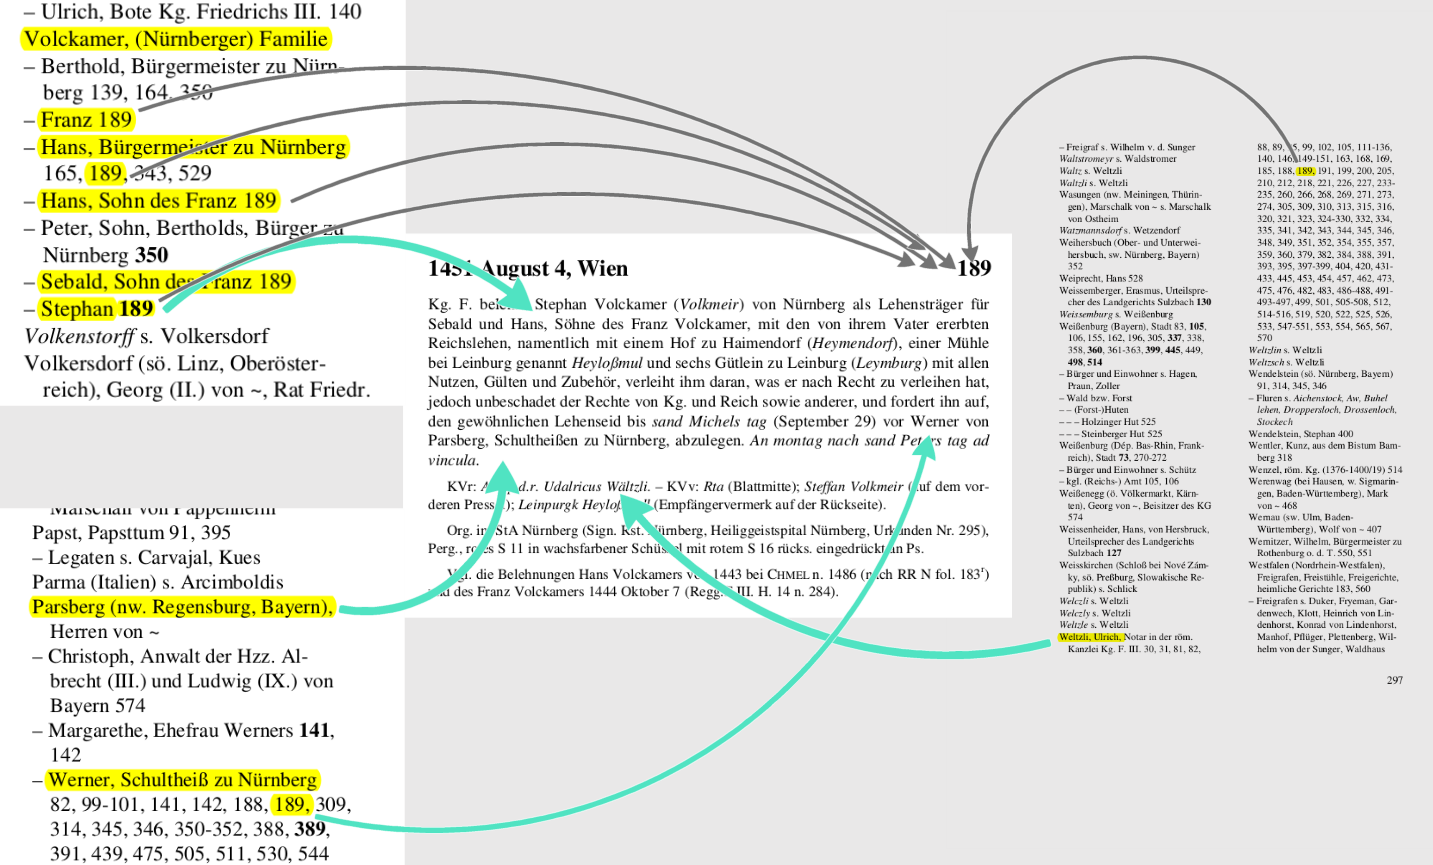
\includegraphics{Bilder/Register-und-Regest-19-189.png}
\caption{Registereinträge im Regest als Grundlage für ein Personennetzwerk.}
\label{registereintraege}
\end{figure}

Allein die Einträge in den Registern der Regesten Kaiser Friedrichs III. sind über 143.000 mal in Regesten genannt. Daraus ergeben sich dann über 460.000 1zu1-Beziehungen, vgl. Abb. \ref{1zu1gephi}.\footnote{Der Cypher-Befehl zur Erstellung der 1zu1-Beziehungen lautet: \emph{MATCH (n1:Registereintrag)-{[}:APPEARS\_IN{]}-\textgreater{}(r:Regest)\textless{}-{[}:APPEARS\_IN{]}-(n2:Registereintrag) MERGE (n1)-{[}:KNOWS{]}-\textgreater{}(n2);} Dabei werden die gerichteten \texttt{KNOWS}-Kanten jeweils in beide Richtungen erstellt. Mit folgendem Befehl lassen sich die \texttt{KNOWS}-Kanten zählen: \emph{MATCH p=()-{[}r:KNOWS{]}-\textgreater{}() RETURN count(p);} Für die Bestimmung der 1zu1-Beziehungen muss der Wert noch durch 2 geteilt werden.}

\begin{figure}[h]
\centering
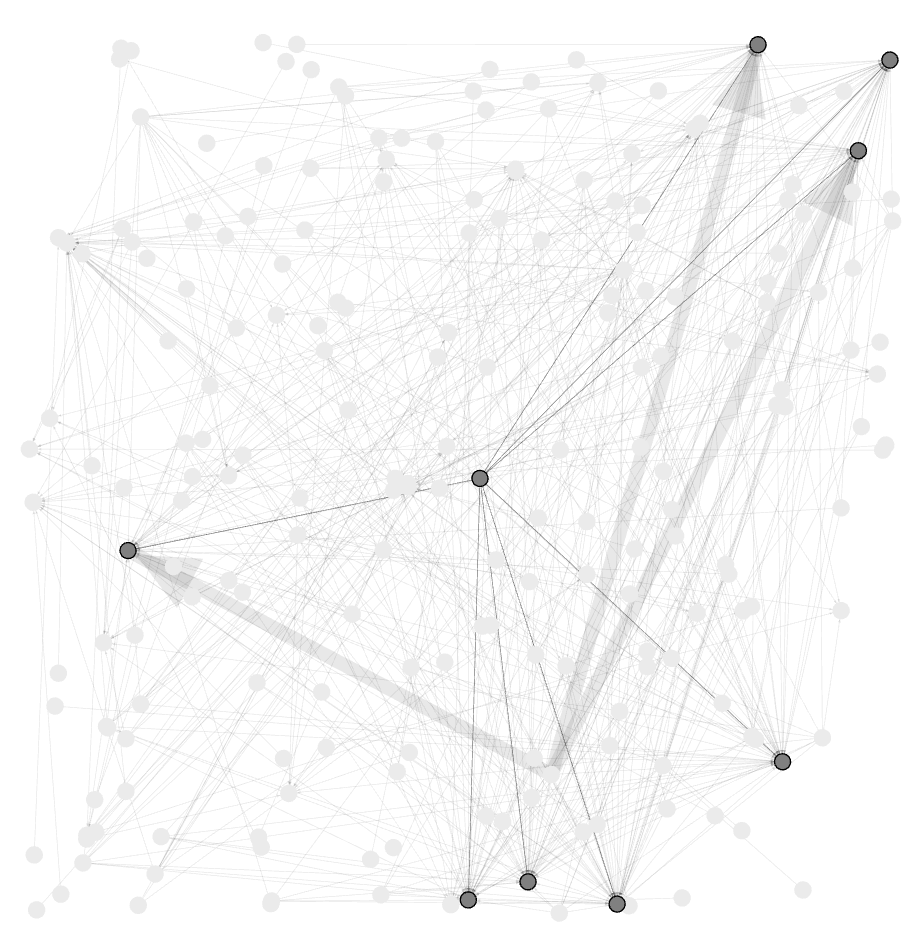
\includegraphics[width=0.8\textwidth]{Bilder/Gephi-Register.png}
\caption{Ausschnitt der 1zu1-Beziehungen in Gephi.}
\label{1zu1gephi}
\end{figure}

In Abb. \ref{chmelvisualisierung} sind die in den Registern des Regestenbandes von Joseph Chmel gewonnenen 1zu1-Beziehungen mit Gephi visualisiert.\footnote{Regesta chronologico-diplomatica Friderici III. Romanorum imperatoris (regis IV.) : Auszug aus den im K.K. Geheimen Haus-, Hof- und Staats-Archive zu Wien sich befindenden Registraturbüchern vom Jahre 1440 - 1493 ; nebst Auszügen aus Original-Urkunden, Manuscripten und Büchern / von Joseph Chmel, Wien 1838 und 1840.}

\begin{figure}[h]
\centering
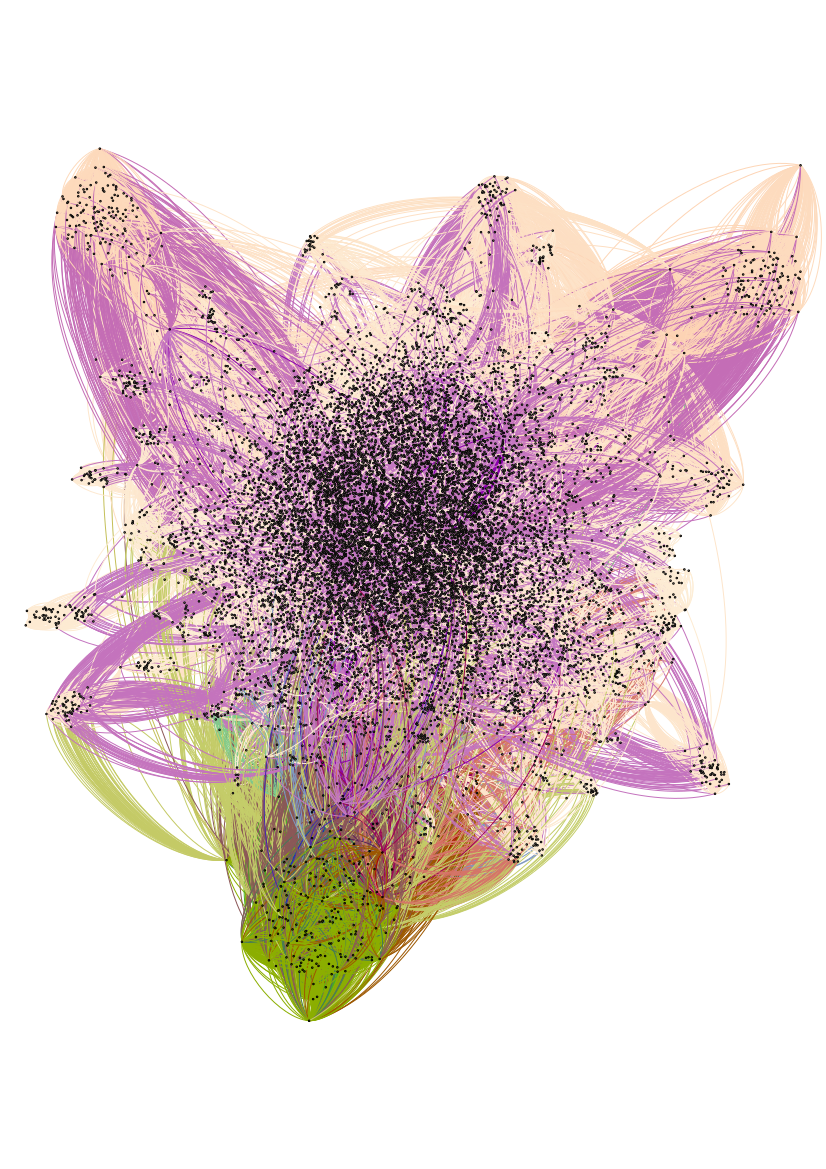
\includegraphics[width=0.8\textwidth]{Bilder/Chmelvisualisierung-v2.png}
\caption{Personennetzwerk aus den Registern der Regesten Chmels, erstellt mit Gephi (Quelle: Kuczera).}
\label{chmelvisualisierung}
\end{figure}

Bei der Analyse ergaben sich aber verschiedene Probleme. Zum einen werden in den Registern auch Kanzleibeamte genannt, die mit der eigentlichen Urkundenhandlung gar nichts zu tun hatten sondern später lediglich ihr Kürzel auf der Urkunde hinterließen. Dies mag archivgeschichtlich interessant sein, für die Urkundenhandlung ist es aber irrelevant. Ein zweites Problem ist der Aufbau des Registers, in dem Orte und Personen in einem Register zusammengefasst werden. Zum einen handelt es sich hierdurch nicht mehr um ein reines Personennetzwerk sondern um ein gemischtes Personen- und Ortsnetzwerk. Zum anderen überragen die über sehr lange Zeit bestehenden Orte, die in ihrer Lebensdauer begrenzten natürlichen Personen in den Netzwerkstrukturen. Schließlich zeigte sich, dass die Algorithmen zur Netzwerkanalyse mit zeitbehaftenen Daten (wie Regesten mit ihrem Ausstellungsdatum) nur schlecht umgehen konnten.

Aus Historikersicht war der Ansatz also weniger zielführend. Jedoch ergaben sich aus Modellierungssicht interessante Einblicke. Um die Netzwerke näher analysieren zu können, wurden kurze Zeitschnitte der Regesten untersucht. Hierfür musste das in Java geschriebene Programm zur Erstellung der Netzwerkdaten jedesmal umgeschrieben werden. Mein Kollege Ulli Meybohm, der das Programm damals betreute, wies mich nach dem wiederholten Umschreiben des Programms darauf hin, dass ich für meine Daten besser eine Graphdatenbank verwenden solle, beispielsweise neo4j. Erste Versuche des Imports der Registerdaten in neo4j erwiesen sich aber als sehr komplex, vgl. Abb. \ref{regestregister}, obwohl das Datenmodell \emph{Person kennt Person} eigentlich relativ einfach ist.

\begin{figure}[h]
\centering
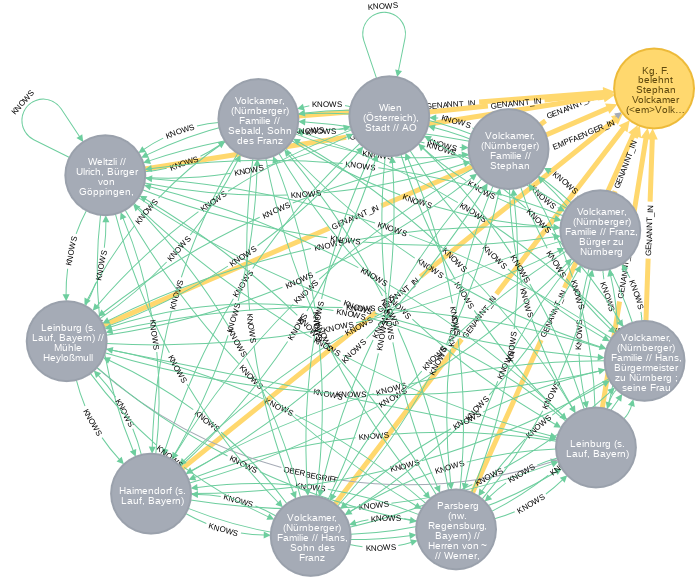
\includegraphics[width=0.7\textwidth]{Bilder/1zu1-Beziehungen-Register-Regest.png}
\caption{Regest und Registereinträge mit \texttt{GENANNT\_IN}-Kanten und den \texttt{KNOWS}-Kanten.}
\label{regestregister}
\end{figure}

Schließlich ergaben Nachfragen bei neo4j, dass bei Problemen mit dem Datenmodell oft einfach ein Typ von Knoten vergessen worden sein könnte. Und tatsächlich wurden in den ersten Modellen die Regestenknoten nicht berücksichtigt. Mit den Regestenknoten im Modell war der Import schließlich mit weniger rechnerischem Aufwand möglich, vgl. Abb. \ref{graphmodellohne}.

\begin{figure}[h]
\centering
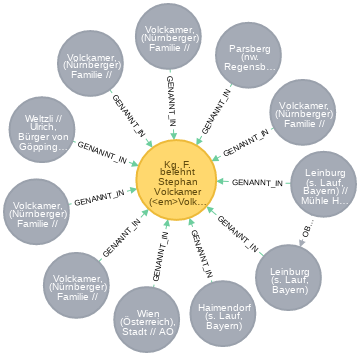
\includegraphics[width=0.6\textwidth]{Bilder/1zu1-Beziehungen-nur-Regest.png}
\caption{Graphmodell ohne \texttt{KNOWS}-Kanten. Diese können bei Bedarf einfach errechnet werden.}
\label{graphmodellohne}
\end{figure}

\hypertarget{zusammenfassung-1}{%
\section{Zusammenfassung}\label{zusammenfassung-1}}

In diesem Kapitel wurde zunächst das Akademieprojekt Regesta Imperii vorgestellt. Seit der Anfang der 2000er Jahre erfolgten Digitalisierung stehen die Regesten unter \url{www.regesta-imperii.de} unter Creative-Commons-Lizenz frei im Internet zur Nutzung zur Verfügung. Für die Auswertung gibt es eine einfache Suchmaske und eine erweiterte Suche. Für die Jahre 2012 und 2013 wurden die Suchstrategien der Nutzer in der Online-Regestensuche untersucht und es zeigte sich, dass sich zwei Nutzungsszenarien unterscheiden lassen, von denen aber nur eines von den aktuellen Suchmasken der Regesta Imperii Online optimal bedient wird. Im zweiten Teil des Kapitels wurden die Visualisierung von Registernetzwerken und die anschließende Modellierung in Graphdatenbanken dargestellt und Nutzungs- und Auswertungsszenarien diskutiert. Im folgenden Kapitel wird die Modellierung von Regesten im Graphen detailliert erklärt.

\hypertarget{regestenmodellierung-im-graphen}{%
\chapter{Regestenmodellierung im Graphen}\label{regestenmodellierung-im-graphen}}

\hypertarget{wie-kommen-die-regesten-in-den-graphen}{%
\section{Wie kommen die Regesten in den Graphen}\label{wie-kommen-die-regesten-in-den-graphen}}

In diesem Abschnitt wird beispielhaft anhand der Regesten Kaiser Heinrichs IV. der Import der Online-Regesten in die Graphdatenbank neo4j durchgespielt.\footnote{Die Einrichtung der Graphdatenbank Neo4j wird erläutert unter \url{https://neo4j.com/docs/operations-manual/current/installation/}. Die Regesten Kaiser Heinrichs IV. umfassen folgende Bände: Böhmer, J. F., Regesta Imperii III. Salisches Haus 1024-1125. Tl. 2: 1056-1125. 3. Abt.: Die Regesten des Kaiserreichs unter Heinrich IV. 1056 (1050) - 1106. 1. Lief.: 1056 (1050) -- 1065, bearb. von Struve, Tilman - Köln (u.a.) (1984). Böhmer, J. F., Regesta Imperii III. Salisches Haus 1024-1125. Tl. 2: 1056-1125. 3. Abt.: Die Regesten des Kaiserreichs unter Heinrich IV. 1056 (1050) - 1106. 2. Lief.: 1065--1075, bearb. von Struve, Tilman unter Mitwirkung von Lubich, Gerhard und Jäckel, Dirk - Köln (u.a.) (2010). Böhmer, J. F., Regesta Imperii III. Salisches Haus 1024-1125. Tl. 2: 1056-1125. 3. Abt.: Die Regesten des Kaiserreichs unter Heinrich IV. 1056 (1050) - 1106. 3. Lief.: 1076--1085, bearb. von Lubich, Gerhard nach Vorarbeiten von Struve, Tilman unter Mitwirkung von Jäckel, Dirk - Köln (u.a.) (2016). Böhmer, J. F., Regesta Imperii III. Salisches Haus 1024-1125. Tl. 2: 1056-1125. 3. Abt.: Die Regesten des Kaiserreichs unter Heinrich IV. 1056 (1050) - 1106. 4. Lief.: 1086--1105/06, bearb. von Lubich, Gerhard nach Vorarbeiten von Brauch, Daniel unter Mitwirkung von Weber, Matthias - Köln (u.a.) (2016). Böhmer, J. F., Regesta Imperii III. Salisches Haus 1024-1125. Tl. 2: 1056-1125. 3. Abt.: Die Regesten des Kaiserreichs unter Heinrich IV. 1056 (1050) - 1106. 5. Lief.: Die Regesten Rudolfs von Rheinfelden, Hermanns von Salm und Konrads (III.). Verzeichnisse, Register, Addenda und Corrigenda, bearbeitet von Lubich, Gerhard unter Mitwirkung von Junker, Cathrin; Klocke, Lisa und Keller, Markus - Köln (u.a.) (2018).} Die Webseite der Regesta Imperii Online basiert auf dem Content-Managment-System typo3, welches auf eine mysql-Datenbank aufbaut. In der Datenbank werden die Regesteninformationen in verschiedenen Tabellen vorgehalten. Die Webseite bietet momentan nur die Möglichkeit, die Regesten über eine REST-Schnittstelle im CEI-XML-Format herunterzuladen. Die CSV-Version, die sich für den Import in die Graphdatenbank anbietet findet sich auf Github: \url{https://github.com/kuczera/GraphReader/raw/master/data/RegH4.csv}. Unter \url{https://github.com/kuczera/GraphReader/raw/master/data/GraphReaderCypher.txt} ist eine Textdatei mit den Listings aller cypher-Befehle erhältlich.

\begin{figure}
\centering
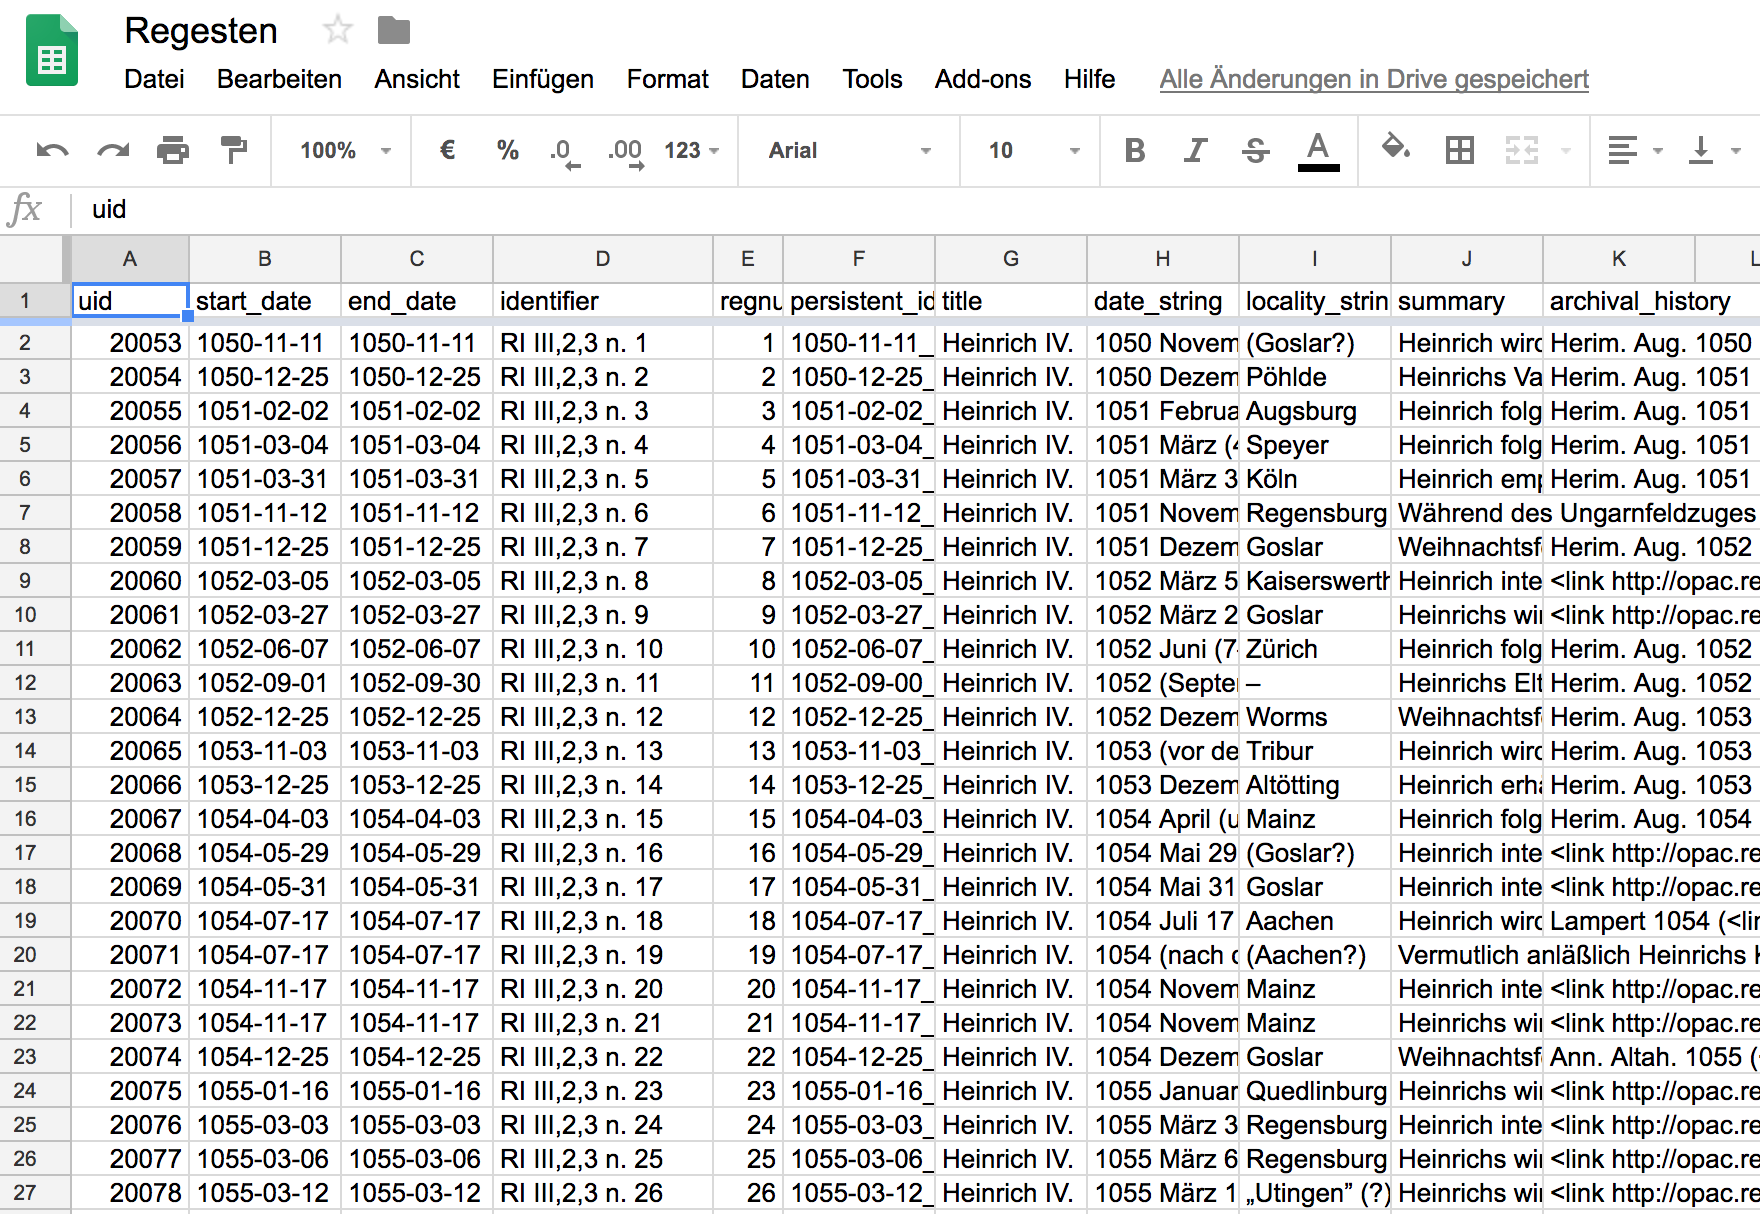
\includegraphics[width=0.6\textwidth]{Bilder/RI2Graph/ReggH4-Regestentabelle.png}
\caption{Regesten als CSV-Datei}
\label{regestenalscsv}
\end{figure}

In der in Abb. \ref{regestenalscsv} dargestellten CSV-Datei finden sich die oben erläuterten einzelnen Elemente der Regesten in jeweils eigenen Spalten. Die Spaltenüberschrift gibt Auskunft zum Inhalt der jeweiligen Spalte.

\hypertarget{import-mit-dem-load-csv-befehl}{%
\subsection{\texorpdfstring{Import mit dem \texttt{LOAD\ CSV}-Befehl}{Import mit dem LOAD CSV-Befehl}}\label{import-mit-dem-load-csv-befehl}}

Mit dem Befehl \texttt{LOAD\ CSV} können die CSV-Dateien mit den Regesten in die Graphdatenbank neo4j importiert werden.\footnote{Zu Installation und ersten Schritten von neo4j vgl. in der Einleitung den Abschnitt zu Installation und Start.} Hierfür muss die Datenbank aber Zugriff auf die CSV-Daten haben. Dies ist einerseits über den im Datenbankverzeichnis vorhandene Ordner \texttt{import} oder über eine URL, unter der die CSV-Datei abrufbar ist, möglich. Da sich die einzelnen Zugriffswege auf den \texttt{import}-Ordner von Betriebssystem zu Betriebssystem unterscheiden, wird hier beispielhaft der Import über eine URL vorgestellt. Hierfür wird ein Webserver benötigt, auf den man die CSV-Datei hochlädt und sich anschließend die Webadresse für den Download der Datei notiert. Für die hier vorgestellten Beispiele werden die Daten über github bereitgestellt:  \url{https://github.com/kuczera/GraphReader/raw/master/data/RegH4.csv}.

\hypertarget{regestenmodellierung-im-graphen-1}{%
\subsection{Regestenmodellierung im Graphen}\label{regestenmodellierung-im-graphen-1}}

Mit dem \texttt{LOAD\ CSV}-Befehl stehen die Informationen der Regestentabelle nun für die weitere Verarbeitung zur Verfügung. Nun muss festgelegt werden, wie diese Informationen im Graphen modelliert werden sollen. Daher wird im nächsten Schritt das Modell der Regesten im Graphen vorgestellt (Abb. \ref{ri2graph}).

\begin{figure}
\centering
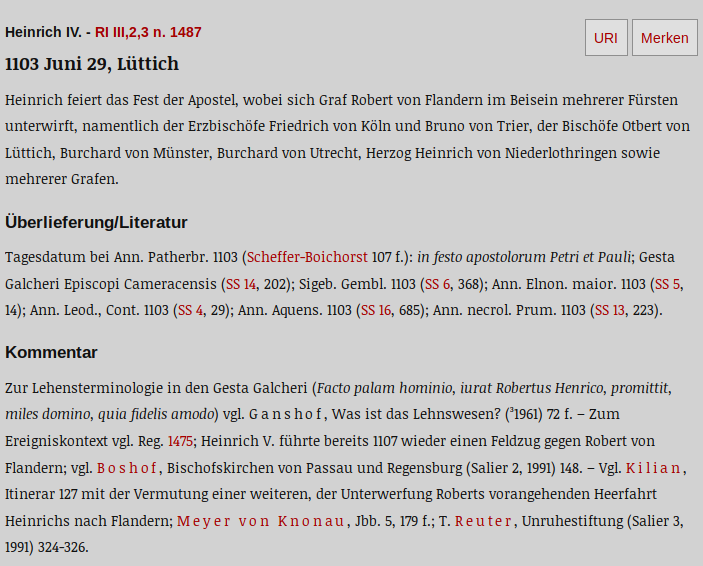
\includegraphics[width=0.6\textwidth]{Bilder/RI2Graph/ReggH4-Nr-1487.png}
\caption{RI III,2,3 n. 1487, in: Regesta Imperii Online, URI: http://www.regesta-imperii.de/id/cf75356b-bd0d-4a67-8aeb-3ae27d1dcefa.}
\label{ri2graph}
\end{figure}

\begin{figure}
\centering
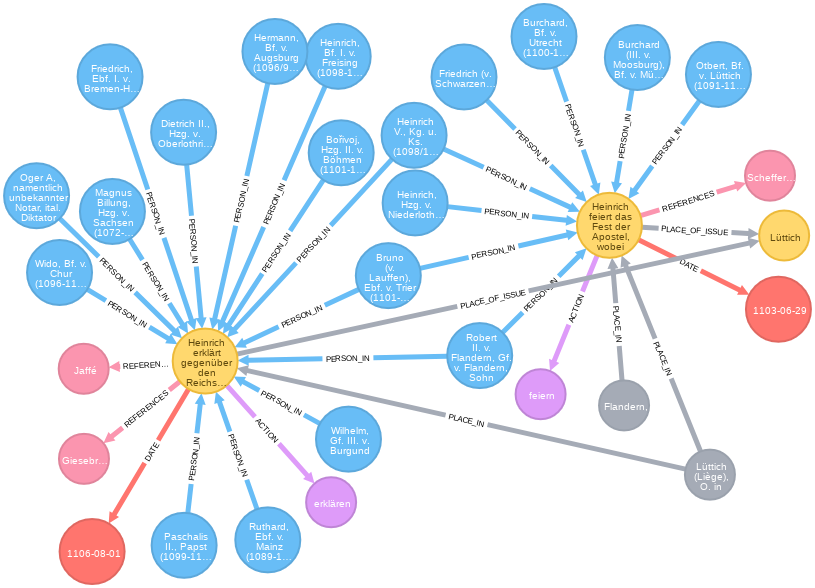
\includegraphics[width=0.6\textwidth]{Bilder/RI2Graph/ReggH4-Nr-1487imGraph.png}
\caption{Das Regest im Graphen.} 
\label{ri2graph2}
\end{figure}

In den Abbildungen \ref{ri2graph} und \ref{ri2graph2} finden sich beispielhaft das Regest RI III,2,3 Nr. 1487, einmal in der Ansicht der Onlineregesten und in der zweiten Abbildung als Modell im Graphen (neben anderen Regesten).

Die gelben Knoten sind die Regesten. Aus den Angaben des Regests werden mit dem o.a. Befehl noch ein Datumsknoten und ein Ortsknoten erstellt. Mit dem ersten \texttt{CREATE}-Befehl werden die Regesten erstellt. Die \texttt{MERGE}-Befehle erzeugen ergänzende Knoten für die Datumsangaben und die Ausstellungsorte. Nun ist es aber so, dass Ausstellungsort und Ausstellungsdatum mehrfach vorkommen können. Daher wird hier nicht der \texttt{CREATE}-Befehl sondern der \texttt{MERGE}-Befehl verwendet. Dieser funktioniert wie der \texttt{CREATE}-Befehl, prüft aber vorher, ob in der Datenbank ein solcher Knoten schon existiert. Falls es ihn noch nicht gibt, wird er erzeugt, wenn es ihn schon gibt, wird er der entsprechenden Variable zugeordnet. Anschließend werden die Kanten zwischen Regestenknoten und Ausstellungsortsknoten sowie Regestenknoten und Datumsknoten erstellt. In der folgenden Tabelle werden die einzelnen Befehle dargestellt und kommentiert.

\hypertarget{indexe-erstellen}{%
\subsection{Indexe Erstellen}\label{indexe-erstellen}}

Bevor nun mit dem Import begonnen wird, ist es für die Beschleunigung des Importprozesses von Vorteil vorher Indexe für häufig genutzte Properties zu erstellen.

\begin{verbatim}
// vorab Index erzeugen -> Import wird schneller
CREATE INDEX ON :Regesta(ident);
CREATE INDEX ON :Regesta(regnum);
CREATE INDEX ON :Regesta(persistentIdentifier);
CREATE INDEX ON :Regesta(registerId);
CREATE INDEX ON :Regesta(heftId);
CREATE INDEX ON :Regesta(placeOfIssue);
CREATE INDEX ON :Regesta(origPlaceOfIssue);
CREATE INDEX ON :Date(startDate);
CREATE INDEX ON :Place(original);
CREATE INDEX ON :Place(normalizedGerman);
CREATE INDEX ON :Lemma(lemma);
CREATE INDEX ON :Literature(literatur);
CREATE INDEX ON :Reference(reference);
CREATE INDEX ON :IndexEntry(registerId);
CREATE INDEX ON :IndexEntry(nodeId);
CREATE INDEX ON :Regesta(latLong);
CREATE INDEX ON :IndexPlace(registerId);
CREATE INDEX ON :IndexEvent(registerId);
CREATE INDEX ON :IndexPerson(registerId);
\end{verbatim}

\hypertarget{erstellen-der-regestenknoten}{%
\subsection{Erstellen der Regestenknoten}\label{erstellen-der-regestenknoten}}

Mit dem folgenden Cypher-Query werden die Regestenknoten in der Graphdatenbank erstellt:

\begin{verbatim}
// Regestenknoten erstellen
LOAD CSV WITH HEADERS FROM "https://github.com/kuczera/GraphReader/raw/master/data/RegH4.csv" AS line
CREATE (r:Regesta {regid:line.persistentIdentifier, text:line.summary,
  archivalHistory:line.archival_history, date:line.date_string,  
  ident:line.identifier,  regnum:line.regnum,
  origPlaceOfIssue:line.locality_string, startDate:line.start_date,
  endDate:line.end_date})
MERGE (d:Date {startDate:line.start_date, endate:line.end_date})
MERGE (r)-[:DATE]->(d)
RETURN count(r);
\end{verbatim}

Im Folgenden werden die einzelnen Teile des Import-Befehls erläutert:

\begin{longtable}[]{@{}lll@{}}
\toprule
\begin{minipage}[b]{0.31\columnwidth}\raggedright
Befehl\strut
\end{minipage} & \begin{minipage}[b]{0.23\columnwidth}\raggedright
Variablen\strut
\end{minipage} & \begin{minipage}[b]{0.37\columnwidth}\raggedright
Bemerkungen\strut
\end{minipage}\tabularnewline
\midrule
\endhead
\begin{minipage}[t]{0.31\columnwidth}\raggedright
\texttt{LOAD\ CSV\ WITH\ HEADERS\ FROM} ``https://github.com/kuczera/ GraphReader/raw/master/ data/RegH4.csv'' AS line\strut
\end{minipage} & \begin{minipage}[t]{0.23\columnwidth}\raggedright
line\strut
\end{minipage} & \begin{minipage}[t]{0.37\columnwidth}\raggedright
Import der CSV-Dateien. Es wird jeweils eine Zeile an die Variable line weitergegeben\strut
\end{minipage}\tabularnewline
\begin{minipage}[t]{0.31\columnwidth}\raggedright
\texttt{CREATE}(r:Regesta \{regid:line.persistentIdentifier, text:line.summary, archivalHistory:line.archival\_history, date:line.date\_string etc. \strut
\end{minipage} & \begin{minipage}[t]{0.23\columnwidth}\raggedright
line.persistent\_ identifier, line.summary etc.\strut
\end{minipage} & \begin{minipage}[t]{0.37\columnwidth}\raggedright
Erstellung des Regestenknotens. Für die weiteren Befehle steht der neu erstellt Regestenknoten unter der Variable \texttt{r} zur Verfügung.\strut
\end{minipage}\tabularnewline
\begin{minipage}[t]{0.31\columnwidth}\raggedright
\texttt{MERGE} (d:Date \{startDate:line.start\_date, endate:line.end\_date\})\strut
\end{minipage} & \begin{minipage}[t]{0.23\columnwidth}\raggedright
line.start\_date und line.end\_date\strut
\end{minipage} & \begin{minipage}[t]{0.37\columnwidth}\raggedright
Es wird geprüft, ob ein Datumsknoten mit der Datumsangabe schon existiert, falls nicht, wird er erstellt. In jedem Fall steht anschließend der Datumsknoten unter der Variable d zur Verfügung.\strut
\end{minipage}\tabularnewline
\begin{minipage}[t]{0.31\columnwidth}\raggedright
\texttt{MERGE} (r)-{[}:HAT\_DATUM{]}-\textgreater{}(d)\strut
\end{minipage} & \begin{minipage}[t]{0.23\columnwidth}\raggedright
\texttt{(r)} ist der Regestenknoten, \texttt{(d)} ist der Datumsknoten\strut
\end{minipage} & \begin{minipage}[t]{0.37\columnwidth}\raggedright
Zwischen Regestenknoten und Datumsknoten wird eine \texttt{HAT\_DATUM}-Kante erstellt.\strut
\end{minipage}\tabularnewline
\bottomrule
\end{longtable}

\hypertarget{erstellen-der-ausstellungsorte}{%
\subsection{Erstellen der Ausstellungsorte}\label{erstellen-der-ausstellungsorte}}

In den Kopfzeilen der Regesten ist, soweit bekannt, der Ausstellungsort der Urkunde vermerkt. Im Rahmen der Arbeiten an den Regesta Imperii Online wurden diese Angaben zusammengestellt und soweit möglich die Orte identifiziert, so dass diese Angabe nun beim Import der Regesten in den Graphen berücksichtigt werden kann. Insgesamt befinden sich in den Regesta Imperii über 12.000 verschiedene Angaben für Ausstellungsorte, wobei sie sich aber auch teilweise auf den gleichen Ort beziehen können (Wie z.B. Aachen, Aquisgrani, Aquisgradi, Aquisgranum, coram Aquisgrano etc.). Allein mit der Identifizierung der 1.000 häufigsten Ortsangaben konnte schon die überwiegende Mehrzahl der Ausstellungsorte georeferenziert werden. Die Daten zur Ortsidentifizierung liegen auch als CSV-Datei vor.

Mit dem folgenden Cypher-Query werden die Ausstellungsorte in die Graphdatenbank importiert:

\begin{verbatim}
// RI-Ausstellungsorte-geo erstellen
LOAD CSV WITH HEADERS FROM "https://github.com/kuczera/GraphReader/raw/master/data/RI_Ortsdaten.csv"
AS line
WITH line
WHERE line.Lat IS NOT NULL
AND line.normalisiertDeutsch IS NOT NULL
MATCH (r:Regesta {origPlaceOfIssue:line.Original})
MERGE (p:Place {normalizedGerman:line.normalisiertDeutsch,
  longitude:line.Long, latitude:line.Lat})
WITH r, p, line
MERGE (r)-[rel:PLACE_OF_ISSUE]->(p)
SET p.wikidataId = line.wikidataId
SET p.name = line.name
SET p.gettyId = line.GettyId
SET p.geonamesId = line.GeonamesId
SET rel.original = line.Original
SET rel.alternativeName = line.Alternativname
SET rel.commentary = line.Kommentar
SET rel.allocation = line.Zuordnung
SET rel.state = line.Lage
SET rel.certainty = line.Sicherheit
SET rel.institutionInCity = line.InstInDerStadt
RETURN count(p);
\end{verbatim}

Da der Import-Query etwas komplexer ist, wird er im folgenden näher erläutert. Nach dem \texttt{LOAD\ CSV\ WITH\ HEADERS\ FROM}-Befehl wird zunächst überprüft, ob der jeweils eingelesene Eintrag in der Spalte \texttt{line.lat} und in der Spalte \texttt{line.normalisiertDeutsch} Einträge hat. Ist dies der Fall, wird überprüft, ob es einen Regestenknoten gibt, der einen Ausstellungsorteintrag hat, der der Angabe in der Spalte \texttt{Original} entspricht. Diese Auswahl ist notwendig, da in der Tabelle die Ausstellungsorte der gesamten Regesta Imperii enthalten sind. Für diesen Import sollen aber nur jene angelegt werden, die für die Regesten Kaiser Heinrichs IV. relevant sind. Mit dem \texttt{MERGE}-Befehl wird der \texttt{Place}-Knoten erstellt (falls es ihn nicht schon gibt) und anschließend mit dem Regestenknoten verknüpft. Schließlich werden noch weitere Details der Ortsangabe im \texttt{Place}-Knoten und in den \texttt{PLACE\_OF\_ISSUE}-Kanten ergänzt.

\hypertarget{koordinaten-der-ausstellungsorte}{%
\subsection{Koordinaten der Ausstellungsorte}\label{koordinaten-der-ausstellungsorte}}

Mit dem folgenden Query werden die Koordinatenangaben zu Höhen- und Breitengraden der Ausstellungsorte (\texttt{Place}-Knoten), die in den Propertys latitude und longitude abgespeichert sind, in der neuen Property LatLong zusammengefasst und in \texttt{point}-Werte umgewandelt. Seit Version 3 kann neo4j mit diesen Werten Abstandsberechnungen durchführen (Mehr dazu siehe unten bei den Auswertungen).

\begin{verbatim}
// Regesten und Ausstellungsorte mit Koordinaten der Ausstellungsorte versehen
MATCH (r:Regesta)-[:PLACE_OF_ISSUE]->(o:Place)
SET r.latLong = point({latitude: tofloat(o.latitude),
  longitude: tofloat(o.longitude)})
SET o.latLong = point({latitude: tofloat(o.latitude),
  longitude: tofloat(o.longitude)})
SET r.placeOfIssue = o.normalizedGerman
SET r.latitude = o.latitude
SET r.longitude = o.longitude;
\end{verbatim}

\hypertarget{ausstellungsdatum}{%
\subsection{Ausstellungsdatum}\label{ausstellungsdatum}}

In den Regesta Imperii Online sind die Datumsangaben der Regesten iso-konform im Format JJJJ-MM-TT (also Jahr-Monat-Tag) abgespeichert. Neo4j behandelt diese Angaben aber als String. Um Datumsberechnungen durchführen zu können, müssen die Strings in neo4j-interne Datumswerte umgerechnet werden. Der Cypher-Query hierzu sieht wie folgt aus:

\begin{verbatim}
// Date in neo4j-Datumsformat umwandeln
MATCH (n:Regesta)
SET n.isoStartDate = date(n.startDate);
MATCH (n:Regesta)
SET n.isoEndDate = date(n.endDate);
MATCH (d:Date)
SET d.isoStartDate = date(d.startDate);
MATCH (d:Date)
SET d.isoEndDate = date(d.endDate);
\end{verbatim}

Zunächst werden mit dem \texttt{MATCH}-Befehl alle Regestenknoten aufgerufen. Anschließend wird für jeden Regestenknoten aus der String-Property \texttt{startDate} die Datumsproperty \texttt{isoStartDate} berechnet und im Regestenknoten abgespeichert. Mit Hilfe der Property können dann Datumsangaben und Zeiträume abgefragt werden (Beispiel hierzu unten in der Auswertung).

\hypertarget{exkurs-1-herrscherhandeln-in-den-regesta-imperii}{%
\section{Exkurs 1: Herrscherhandeln in den Regesta Imperii}\label{exkurs-1-herrscherhandeln-in-den-regesta-imperii}}

Bisher wurden beim Import der Regesten in den Graphen nur die in den Online-Regesten bereits angelegten Angaben importiert. Im folgenden Schritt werden nun in einem kleinen Exkurs die Regestentexte selbst analysiert und anschließend die Graphdatenbank um eine weitere Informationsebene ergänzt. Regesten sind in ihrer Struktur stark formalisiert. Meist wird mit dem ersten Verb im Regest das Herrscherhandeln beschrieben. Um dies auch digital auswerten zu können, haben wir in einem kleinen Testprojekt mit Hilfe des \href{http://www.cis.uni-muenchen.de/~schmid/tools/TreeTagger/}{Stuttgart-München Treetaggers}\footnote{Zum Treetagger vgl. http://www.cis.uni-muenchen.de/\textasciitilde{}schmid/tools/TreeTagger/.} aus jedem Regest das erste Verb extrahiert und normalisiert. Die Ergebnisse sind einsehbar unter https://github.com/kuczera/GraphReader/raw/master/data/ReggH4-Verben.csv. Diese Tabelle wird mit dem folgenden Cypher-Query in die Graphdatenbank eingelesen.

\begin{verbatim}
// ReggH4-Herrscherhandeln
LOAD CSV WITH HEADERS FROM "https://github.com/kuczera/GraphReader/raw/master/data/ReggH4-Verben.csv"
AS line FIELDTERMINATOR ','
MATCH (r:Regesta{ident:line.regid})
MERGE (l:Lemma{lemma:line.Lemma})
MERGE (r)-[:ACTION]->(l);
\end{verbatim}

Dabei wird zunächst mit dem \texttt{MATCH}-Befehl das jeweilige Regest gesucht, anschließend mit dem \texttt{MERGE}-Befehl der \texttt{Lemma}-Knoten für das Herrscherhandeln angelegt (falls noch nicht vorhanden) und schließlich der \texttt{Regesta}-Knoten mit dem \texttt{Lemma}-Knoten über eine \texttt{ACTION}-Kante verbunden. In Abb. \ref{herrscherhandeln} ist ein Ausschnitt mit Regesten und den verknüpften Lemmaknoten dargestellt.

\begin{figure}
\centering
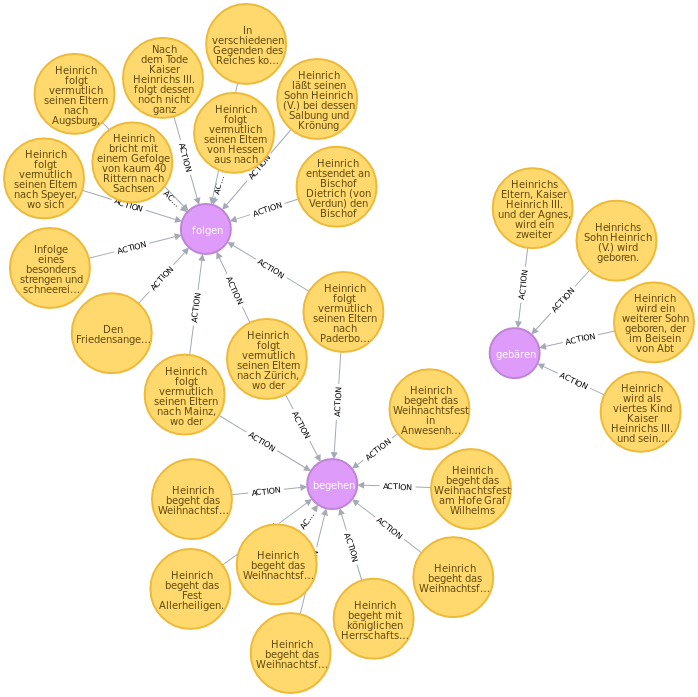
\includegraphics[width=0.6\textwidth]{Bilder/RI2Graph/ReggH4-Action.png}
\caption{Herrscherhandeln im Graphen.}
\label{herrscherhandeln}
\end{figure}

\hypertarget{zitationsnetzwerke-in-den-regesta-imperii}{%
\section{Zitationsnetzwerke in den Regesta Imperii}\label{zitationsnetzwerke-in-den-regesta-imperii}}

In vielen Online-Regesten ist die zitierte Literatur mit dem \href{http://opac.regesta-imperii.de/lang_de/}{Regesta-Imperii-Opac} verlinkt. Da es sich um URLs handelt, sind diese Verweise eindeutig. Andererseits lassen sie sich mit regulären Ausdrücken aus den Regesten extrahieren. Mit folgendem Query werden aus den Überlieferungsteilen der Regesten die mit dem Opac verlinkten Literaturangaben extrahiert und jede Literaturangabe als \texttt{Refernce}-Knoten angelegt. Für den folgenden Befehl muss die APOC-Bibliothek in neo4j installiert sein: \url{https://neo4j-contrib.github.io/neo4j-apoc-procedures/#_installation_with_neo4j_desktop}.

\begin{verbatim}
// ReggH4-Literaturnetzwerk erstellen
MATCH (reg:Regesta)
WHERE reg.archivalHistory CONTAINS "link"
UNWIND apoc.text.regexGroups(reg.archivalHistory,
"<link (\\S+)>(\\S+)</link>") as link
MERGE (ref:Reference {url:link[1]})
ON CREATE SET ref.title=link[2]
MERGE (reg)-[:REFERENCES]->(ref);
\end{verbatim}

Da dies mit dem \texttt{MERGE}-Befehl geschieht, wird in der Graphdatenbank jeder Literaturtitel nur einmal angelegt. Anschließend werden die \texttt{Reference}-Knoten mit den Regesten über \texttt{REFERENCES}-Kanten verbunden. Zu den Auswertungsmöglichkeiten vgl. unten den Abschnitt zu den \protect\hyperlink{ux5cux23Auswertungsperspektiven}{Auswertungsperspektiven}.

\hypertarget{import-der-registerdaten-in-die-graphdatenbank}{%
\section{Import der Registerdaten in die Graphdatenbank}\label{import-der-registerdaten-in-die-graphdatenbank}}

\hypertarget{vorbereitung-der-registerdaten}{%
\subsection{Vorbereitung der Registerdaten}\label{vorbereitung-der-registerdaten}}

Register spielen für die Erschließung von gedrucktem Wissen eine zentrale Rolle, da dort in alphabetischer Ordnung die im Werk vorkommenden Entitäten (z.B. Personen und Orte) hierarchisch gegliedert aufgeschlüsselt werden. Für die digitale Erschließung der Regesta Imperii sind Register von zentraler Bedeutung, da mit ihnen die in den Regesten vorkommenden Personen und Orte bereits identifiziert vorliegen. Für den Import in die Graphdatenbank wird allerdings eine digitalisierterte Fassung des Registers benötigt. Im Digitalisierungsprojekt Regesta Imperii Online wurden Anfang der 2000er Jahre auch die gedruckt vorliegenden Register digitalisiert. Sie dienen nun als Grundlage für die digitale Registererschließung der Regesta Imperii. Im hier gezeigten Beispiel werden die Regesten Kaiser Heinrichs IV. und das dazugehörige Register importiert. Da der letzte Regestenband der Regesten Kaiser Heinrichs IV. mit dem Gesamtregister erst vor kurzem gedruckt wurde, liegen hier aktuelle digitale Fassung von Registern und Regesten vor. Die für den Druck in Word erstellte Registerfassung wird hierfür zunächst in eine hierarchisch gegliederte XML-Fassung konvertiert (vgl. Abb. \ref{ausschnittxml}), damit die Registerhierarchie auch maschinenlesbar abgelegt ist.

\begin{figure}
\centering
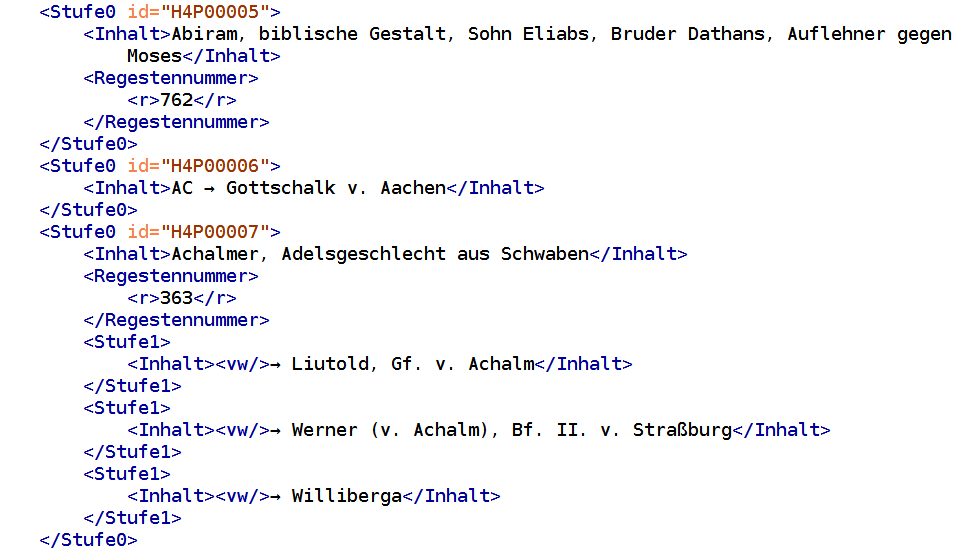
\includegraphics{Bilder/RI2Graph/XML-Register.png}
\caption{Ausschnitt aus dem XML-Register der Regesten Heinrichs IV.}
\label{ausschnittxml}
\end{figure}

In der XML-Fassung sind die inhaltlichen Bereiche und die Abschnitte für die Regestennummern jeweils extra in die Tags \texttt{\textless{}Inhalt\textgreater{}} und \texttt{\textless{}Regestennummer\textgreater{}} eingefasst. Innerhalb des Elements \texttt{\textless{}Regestennummer\textgreater{}} ist dann nochmal jede einzelne Regestennummer in \texttt{\textless{}r\textgreater{}}-Tags eingefasst. Die aus dem gedruckten Register übernommenen Verweise sind durch ein leeres \texttt{\textless{}vw/\textgreater{}}-Element gekennzeichnet.

Die in XML vorliegenden Registerdaten werden anschließend mit Hilfe von TuStep in einzelne CSV-Tabellen zerlegt.

\begin{figure}
\centering
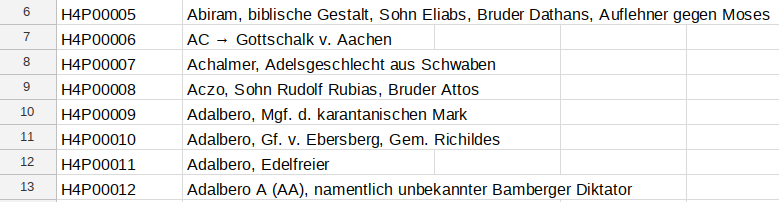
\includegraphics{Bilder/RI2Graph/RegisterH4-Tabelle-Entitaeten.png}
\caption{Ausschnitt der Entitätentabelle des Registers der Regesten Heinrichs IV.}
\label{entitaeten}
\end{figure}

In einer Tabelle werden alle Entitäten aufgelistet und jeweils mit einer ID versehen (Abb. \ref{entitaeten}).

\begin{figure}
\centering
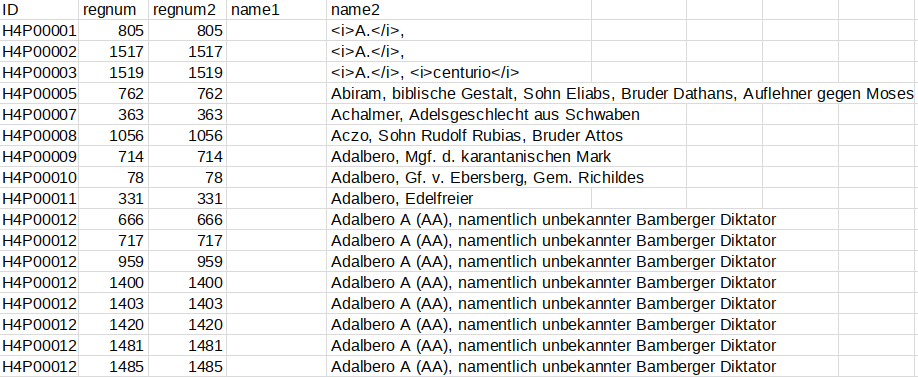
\includegraphics{Bilder/RI2Graph/RegisterH4-GENANNT.png}
\caption{Ausschnitt der Verknüpfungstabelle des Registers der Regesten Heinrichs IV.} 
\label{verknuepfung}
\end{figure}

In der anderen Tabelle werden die Verknüpfungen zwischen Registereinträgen und den Regesten aufgelistet (Abb. \ref{verknuepfung}). Der Registereintrag Adalbero kommt in mehreren Regesten vor. Da das Register der Regesten Heinrichs IV. nur zwei Hierarchiestufen enthält, in denen beispielsweise verschiedene Amtsphasen ein und derselben Person unterschieden werden, wurden diese beim Import zusammengefasst.\footnote{Vgl. die Vorbemerkung zum Register in Böhmer, J. F., Regesta Imperii III. Salisches Haus 1024-1125. Tl. 2: 1056-1125. 3. Abt.: Die Regesten des Kaiserreichs unter Heinrich IV. 1056 (1050) - 1106. 5. Lief.: Die Regesten Rudolfs von Rheinfelden, Hermanns von Salm und Konrads (III.). Verzeichnisse, Register, Addenda und Corrigenda, bearbeitet von Lubich, Gerhard unter Mitwirkung von Junker, Cathrin; Klocke, Lisa und Keller, Markus - Köln (u.a.) (2018), S. 291.} Damit gibt es pro Person jeweils nur einen Knoten.

\hypertarget{import-der-registerdaten-in-die-graphdatenbank-1}{%
\subsection{Import der Registerdaten in die Graphdatenbank}\label{import-der-registerdaten-in-die-graphdatenbank-1}}

Im Gegensatz zu den Regesten Kaiser Friedrichs III., bei denen Orte und Personen in einem Register zusammengefasst sind, haben die Regesten Kaiser Heinrich IV. getrennte Orts- und Personenregister. Die digitalisierten Registerdaten können als Excel- \url{https://github.com/kuczera/GraphReader/raw/master/data/RegisterH4.xlsx} oder als  Openofficedatei \url{https://github.com/kuczera/GraphReader/raw/master/data/RegisterH4.ods} heruntergeladen werden.  In dem Tabellendokument befinden sich insgesamt drei Tabellen. In der Tabelle \texttt{Personen} sind die Einträge des Personenregisters aufgelistet und in der Tabelle \texttt{Orte} befindet sich die Liste aller Einträge des Ortsregisters. Schließlich enthält die Tabelle \texttt{APPEARS\_IN} Information dazu, welche Personen oder Orte in welchen Regesten genannt sind. Der folgende Cypher-Query importiert die Einträge der Personentabelle in die Graphdatenbank und erstellt für jeden Eintrag einen Knoten vom Typ \texttt{:IndexPerson}:

\begin{verbatim}
// Registereinträge Personen erstellen
LOAD CSV WITH HEADERS FROM "https://github.com/kuczera/GraphReader/raw/master/data/RegisterH4-IndexPerson.csv"
AS line
CREATE (:IndexPerson {registerId:line.ID, name1:line.name1});
\end{verbatim}

Mit dem folgenden Cypher-Query werden nach dem gleichen Muster aus der Tabelle \texttt{Orte} die Ortseinträge in die Graphdatenbank importiert.

\begin{verbatim}
// Registereinträge Orte erstellen
LOAD CSV WITH HEADERS FROM "https://github.com/kuczera/GraphReader/raw/master/data/RegisterH4-IndexPlace.csv"
AS line
CREATE (:IndexPlace {registerId:line.ID, name1:line.name1});
\end{verbatim}

Die beiden Befehle laden die CSV-Daten und übergeben die Daten zeilenweise an die weiteren Befehle (Hier an den \texttt{MATCH}- und den \texttt{CREATE}-Befehl). Im nächsten Schritt werden nun mit den Daten der \texttt{APPEARS\_IN}-Tabelle die Verknüpfungen zwischen den Registereinträgen und den Regesten erstellt.

\begin{verbatim}
// PLACE_IN-Kanten für Orte erstellen
LOAD CSV WITH HEADERS FROM "RegisterH4-Place-APPEARS_IN.csv"
AS line
MATCH (from:IndexPlace {registerId:line.ID})
MATCH (to:Regesta {regnum:line.regnum2})
CREATE (from)-[:PLACE_IN {regnum:line.regnum,
  name1:line.name1, name2:line.name2}]->(to);
\end{verbatim}

Mit zwei \texttt{MATCH}-Befehlen werden jeweils das Regest und der Registereintrag aufgerufen und mit dem \texttt{CREATE}-Befehl eine \texttt{PLACE\_IN}-Kante zwischen den beiden Knoten angelegt, die als Attribute den Inhalt der Spalten \texttt{name1} und \texttt{name2} erhält. Analog werden die Verknüpfungen zwischen Regestenknoten und Personenknoten angelegt:

\begin{verbatim}
// PERSON_IN-Kanten für Person erstellen
LOAD CSV WITH HEADERS FROM "RegisterH4-Person-APPEARS_IN.csv"
AS line
MATCH (from:IndexPerson {registerId:line.ID}),
(to:Regesta {regnum:line.regnum2})
CREATE (from)-[:PERSON_IN {regnum:line.regnum, name1:line.name1,
  name2:line.name2}]->(to);
\end{verbatim}

\hypertarget{exkurs-2-die-hierarchie-des-registers-der-regesten-kaiser-friedrichs-iii.}{%
\section{Exkurs 2: Die Hierarchie des Registers der Regesten Kaiser Friedrichs III.}\label{exkurs-2-die-hierarchie-des-registers-der-regesten-kaiser-friedrichs-iii.}}

In anderen Registern der Regesta Imperii, wie beispielsweise den Regesten Kaiser Friedrichs III., sind teilweise fünf oder mehr Hierarchiestufen vorhanden, die jeweils auch Entitäten repräsentieren (vgl. Abb. \ref{registerbamberg}).

\begin{figure}
\centering
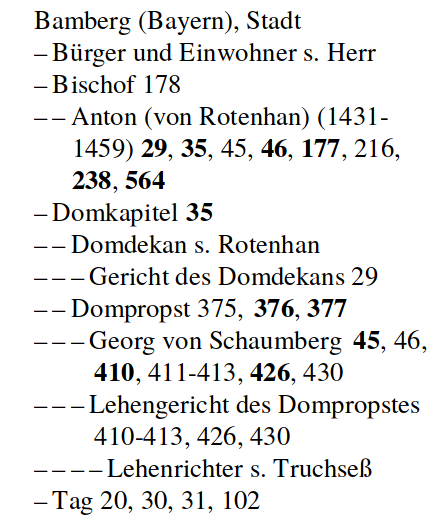
\includegraphics{Bilder/RI2Graph/ReggF3-Registerhierarchie.png}
\caption{Ausschnitt aus dem Register des Heftes 19 der Regesten Kaiser Friedrichs III.}
\label{registerbamberg}
\end{figure}

In diesen Fällen müssen die Hierarchien auch in der Graphdatenbank abgebildet werden, was durch zusätzliche Verweise auf die ggf. vorhandenen übergeordneten Registereinträge möglich wird.

\begin{figure}
\centering
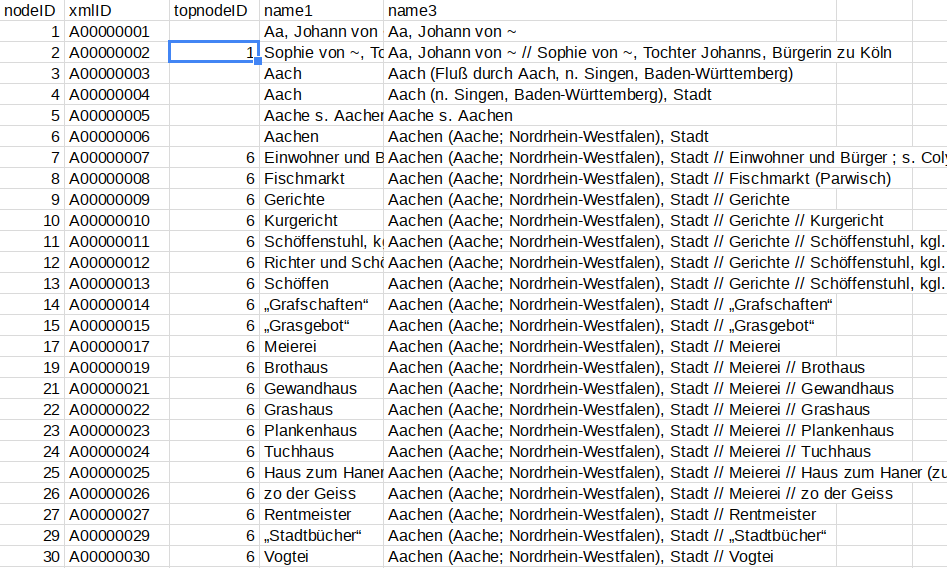
\includegraphics{Bilder/RI2Graph/RegisterF3-Hierarchie.png}
\caption{Ausschnitt der Entitätentabelle des Registers der Regesten Friedrichs III.}
\label{entitaetenaachen}
\end{figure}

Im Tabellenausschnitt (Abb. \ref{entitaetenaachen})wird jedem Registereintrag in der ersten Spalte eine \texttt{nodeID} als eindeutige Kennung zugewiesen. Bei Registereinträgen, die kein Hauptlemma sind, enthält die dritte Spalte \texttt{topnodeID} den Verweis auf die eindeutige Kennung \texttt{nodeID} des übergeordneten Eintrages. Beim Import in die Graphdatenbank wird diese Hierarchie über \texttt{CHILD\_OF}-Kanten abgebildet, die vom untergeordneten Eintrag auf das übergeordnete Lemma verweisen. Damit ist die komplette Registerhierarchie im Graphen abgebildet. In der Spalte \texttt{name1} ist das Lemma angegeben. In der Spalte \texttt{name3} ist zusätzlich zum Lemma noch der gesamte Pfad vom Hauptlemma bis zum Registereintrag, jeweils mit Doppelslashes (\texttt{//}) getrennt. Bei tiefer gestaffelten Registern ist teilweise ohne Kenntnis der übergeordneten Einträge eine eindeutige Identifizierung eines Eintrages nicht möglich. So wird in Zeile 17 der o.a. Abbildung allein mit der Angabe aus der Spalte \texttt{name1} nicht klar, um welche \texttt{Meierei} es sich handelt. Mit dem kompletten Pfad des Registereintrages in der Spalte \texttt{name3} wird dagegen deutlich, dass die Aachener \texttt{Meierei} gemeint ist.

\hypertarget{auswertungsperspektiven}{%
\section{Auswertungsperspektiven}\label{auswertungsperspektiven}}

\hypertarget{personennetzwerke-in-den-registern}{%
\subsection{Personennetzwerke in den Registern}\label{personennetzwerke-in-den-registern}}

\hypertarget{graf-robert-ii.-von-flandern-in-seinem-netzwerk}{%
\subsubsection{Graf Robert II. von Flandern in seinem Netzwerk}\label{graf-robert-ii.-von-flandern-in-seinem-netzwerk}}

Nach dem Import können nun die Online-Regesten und die Informationen aus den Registern der Regesten Kaiser Heinrichs IV. in einer Graphdatenbank aus einer Vernetzungsperspektive abgefragt werden.\footnote{Die nun folgenden Abfragen sind zum Teil einer Präsentation entnommen, die für die Summerschool der \href{https://www.digitale-akademie.de}{Digitalen Akademie} im Rahmen des \href{https://www.mainzed.org/de}{Mainzed} entwickelt wurden. Die Präsentation findet sich unter der URL \url{https://digitale-methodik.adwmainz.net/mod5/5c/slides/graphentechnologien/RI.html}.}

Ausgangspunkt ist der Registereintrag von \href{https://de.wikipedia.org/wiki/Robert_II._(Flandern)}{Graf Robert II. von Flandern}. Diesen Knoten finden wir mit folgendem Query.

\begin{verbatim}
// Robert II. von Flandern
MATCH (n:IndexPerson) WHERE n.registerId = 'H4P01822'
RETURN *;
\end{verbatim}

Mit einem Doppelklick auf den \texttt{IndexPerson}-Knoten öffnen sich alle \texttt{Regesta}-Knoten, in denen Robert genannt ist. Klickt man nun wiederum alle Regestenknoten doppelt an, sieht man alle Personen und Orte, mit denen Robert gemeinsam in den Regesten genannt ist.

Dies kann auch in einem Cypher-Query zusammengefasst werden.

\begin{verbatim}
// Robert II. von Flandern mit Netzwerk
MATCH (n:IndexPerson)-[:PERSON_IN]->
(r:Regesta)<-[:PERSON_IN]-
(m:IndexPerson)
WHERE n.registerId = 'H4P01822'
RETURN *;
\end{verbatim}

In  Abb. \ref{robertundpersonen} wird das Ergebnis dargestellt.

\begin{figure}
\centering
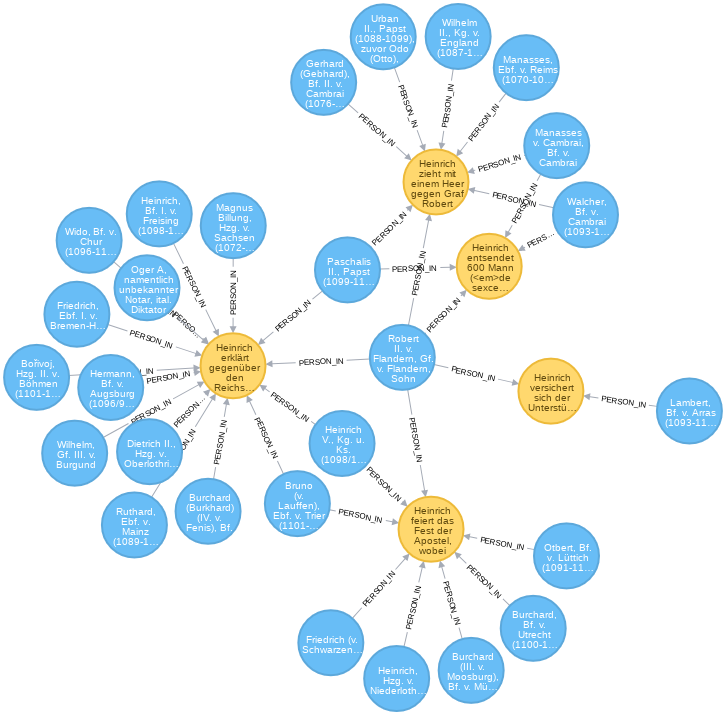
\includegraphics{Bilder/RI2Graph/RobertVonFlandernMitRegesten.png}
\caption{Robert mit den Personen, mit denen er gemeinsam in Regesten genannt wird.}
\label{robertundpersonen}
\end{figure}

Hier wird der \texttt{MATCH}-Befehl um einen Pfad über \texttt{PERSON\_IN}-Kanten zu \texttt{Regesta}-Knoten ergänzt, von denen jeweils eine \texttt{PERSON\_IN}-Kante zu den anderen, in den Regesten genannten \texttt{IndexPerson}-Knoten führt.

Nimmt man noch eine weitere Ebene hinzu, wächst die Ergebnismenge stark an (Abb. \ref{robertundmehrpersonen}). Der folgende Query kann daher je nach Rechnerleistung etwas länger dauern.

\begin{verbatim}
// Robert II. von Flandern mit Netzwerk und Herrscherhandeln (viel)
MATCH
(n1:IndexPerson)-[:PERSON_IN]->(r1:Regesta)<-[:PERSON_IN]-
(n2:IndexPerson)-[:PERSON_IN]->(r2:Regesta)<-[:PERSON_IN]-
(n3:IndexPerson)
WHERE n1.registerId = 'H4P01822'
RETURN *;
\end{verbatim}

\begin{figure}
\centering
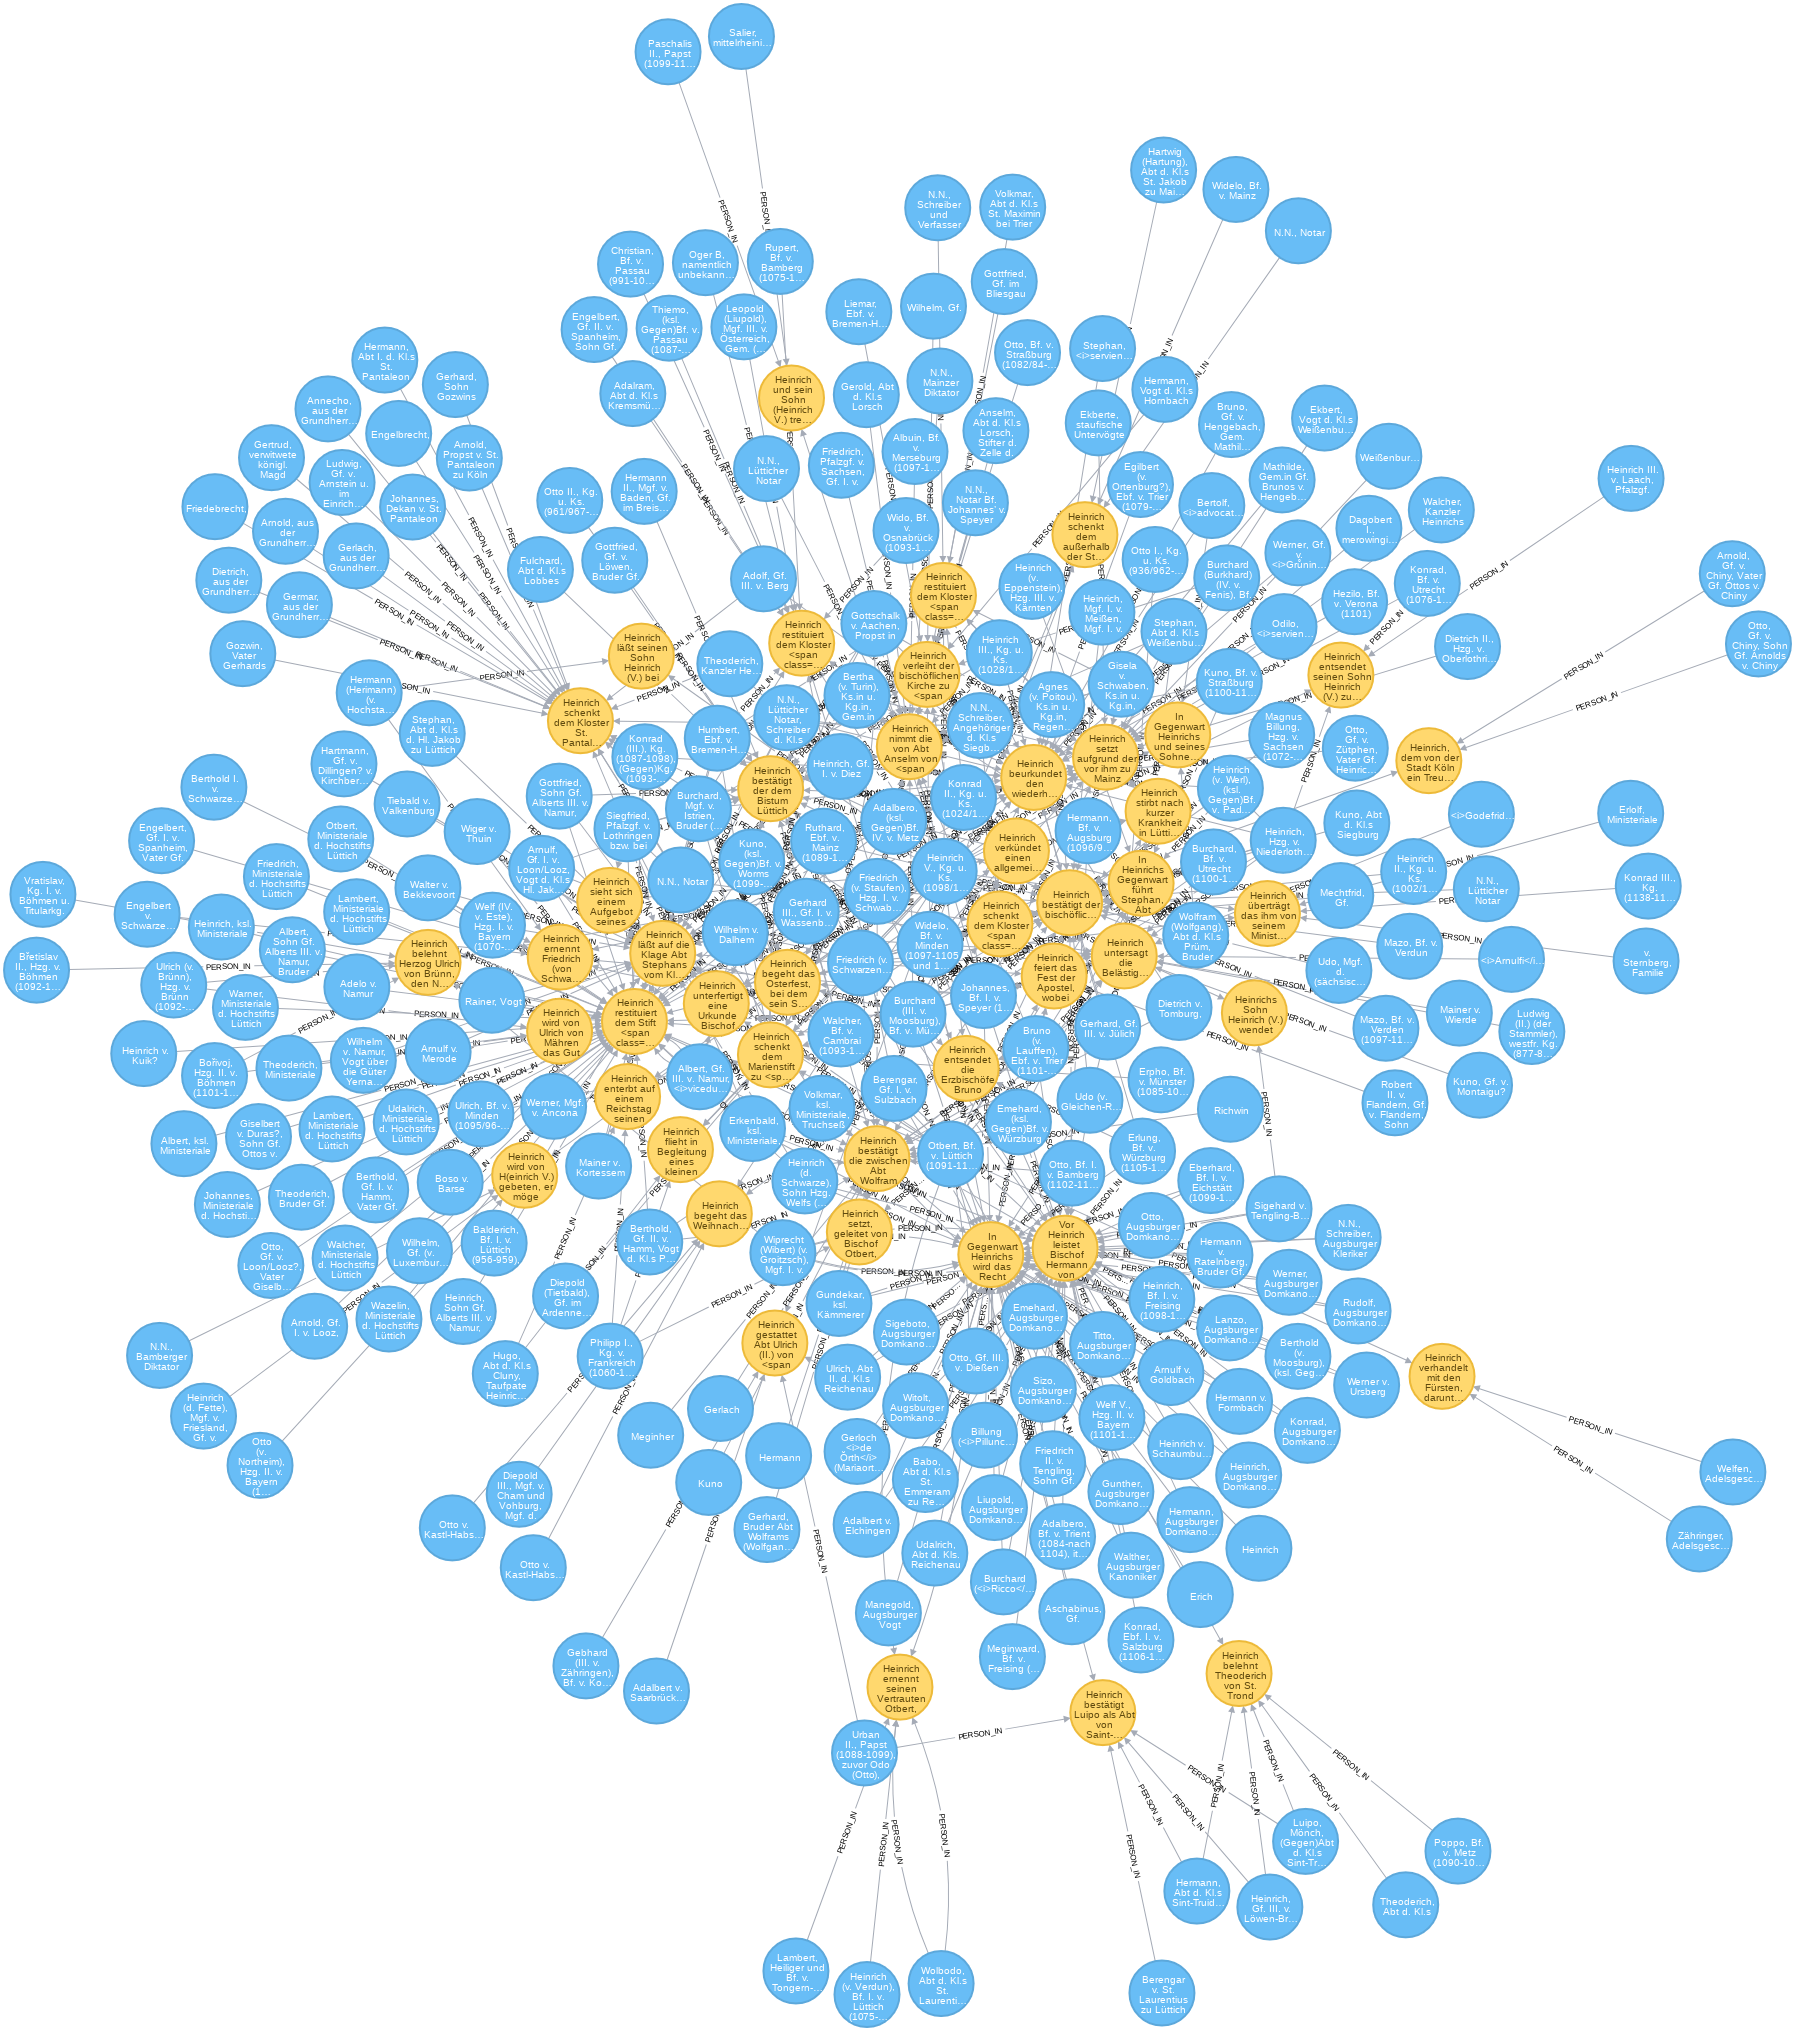
\includegraphics{Bilder/RI2Graph/Robert-viel.png}
\caption{Robert mit Personen, die wiederum mit Personen gemeinsam in Regesten genannt sind.}
\label{robertundmehrpersonen}
\end{figure}

\hypertarget{graf-robert-ii.-von-flandern-und-herzog-heinrich-von-niederlothringen}{%
\subsubsection{Graf Robert II. von Flandern und Herzog Heinrich von Niederlothringen}\label{graf-robert-ii.-von-flandern-und-herzog-heinrich-von-niederlothringen}}

In der Graphdatenbank ist es über die Exploration der Beziehungen einer Person hinaus möglich, explizit die Verbindungen von zwei Personen abzufragen. In unserem nächsten Beispiel suchen wir jene Regesten, in denen \href{https://de.wikipedia.org/wiki/Robert_II._(Flandern)}{Graf Robert II. von Flandern} und \href{https://de.wikipedia.org/wiki/Heinrich_I._(Limburg)}{Herzog Heinrich von Niederlothringen} gemeinsam genannt sind.

\begin{verbatim}
// Robert II. von Flandern und Herzog Heinrich von Niederlothringen mit Netzwerk
MATCH
(n:IndexPerson)-[:PERSON_IN]->
(r:Regesta)<-[:PERSON_IN]-(m:IndexPerson)
WHERE n.registerId = 'H4P01822'
AND m.registerId = 'H4P00926'
RETURN *;
\end{verbatim}

\begin{figure}
\centering
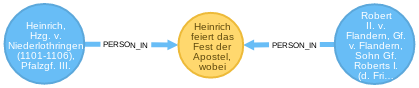
\includegraphics{Bilder/RI2Graph/RobertundHeinrich.png}
\caption{Robert und Heinrich sind in einem Regest gemeinsam genannt.}
\label{robertundheinrich}
\end{figure}

Es zeigt sich, dass Robert und Heinrich in einem Regest gemeinsam genannt sind (Abb. \ref{robertundheinrich}).

Und dieses \href{http://www.regesta-imperii.de/id/cf75356b-bd0d-4a67-8aeb-3ae27d1dcefa}{Regest} berichtet von der Unterwerfung Roberts unter Heinrich IV.\footnote{Vgl. RI III,2,3 n. 1487.}

\begin{quote}
Heinrich feiert das Fest der Apostel, wobei sich Graf Robert von Flandern im Beisein mehrerer Fürsten unterwirft, namentlich der Erzbischöfe Friedrich von Köln und Bruno von Trier, der Bischöfe Otbert von Lüttich, Burchard von Münster, Burchard von Utrecht, Herzog Heinrich von Niederlothringen sowie mehrerer Grafen.
\end{quote}

Möglicherweise haben beide aber gemeinsame Bekannte, also Personen mit denen sowohl Heinrich als auch Robert in unterschiedlichen Regesten gemeinsam genannt sind. Hierfür wird der Cypher-Query um eine Ebene erweitert.

\begin{verbatim}
// Robert und Heinrich mit allen gemeinsamen Personen und Regesten
MATCH (n1:IndexPerson)
-[:PERSON_IN]->(r1:Regesta)<-[:PERSON_IN]-
(n2:IndexPerson)-[:PERSON_IN]->(r2:Regesta)
<-[:PERSON_IN]-(n3:IndexPerson)
WHERE n1.registerId = 'H4P00926'
AND n3.registerId = 'H4P01822'
RETURN *;
\end{verbatim}

\begin{figure}
\centering
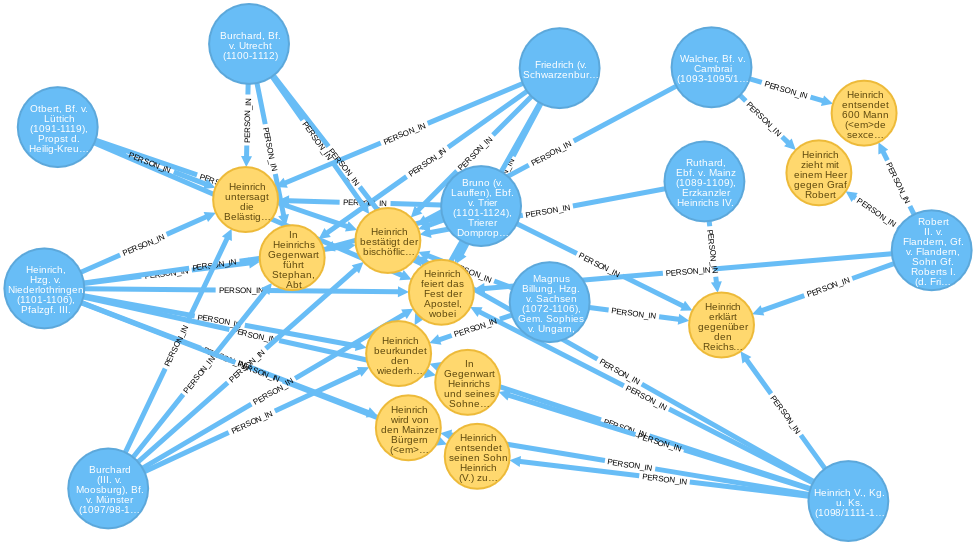
\includegraphics{Bilder/RI2Graph/RobertundHeinrichMitBrokern.png}
\caption{Robert und Heinrich mit den gemeinsamen Bekanntschaften.}
\label{robertundheinrichundmehr}
\end{figure}

Ein erster Blick auf das Ergebnis (Abb. \ref{robertundheinrichundmehr}) zeigt, dass Heinrich allgemein besser vernetzt ist. Für die weitere Analyse ihres Verhältnisses ist nun die Lektüre der angegebenen Regesten notwendig. Hierfür lässt sich das Ergebnis noch etwas weiter aufbereiten, indem die zwischen den Personen liegenden Regesten in \texttt{KNOWS}-Kanten umgewandelt werden, die als zusätzliche Information die Angaben zu den Regesten enthalten.

\begin{verbatim}
// Rausrechnen der dazwischenliegenden Knoten
MATCH
(startPerson:IndexPerson)-[:PERSON_IN]->
(regest:Regesta)<-[:PERSON_IN]-(endPerson:IndexPerson)
WHERE startPerson.registerId in ['H4P01822', 'H4P00926']
WITH startPerson, endPerson, count(regest) as anzahl,
collect(regest.ident) as idents
CALL apoc.create.vRelationship(startPerson, "KNOWS",
{anzahl:anzahl, regesten:idents}, endPerson) YIELD rel
RETURN startPerson, endPerson, rel;
\end{verbatim}

\begin{figure}
\centering
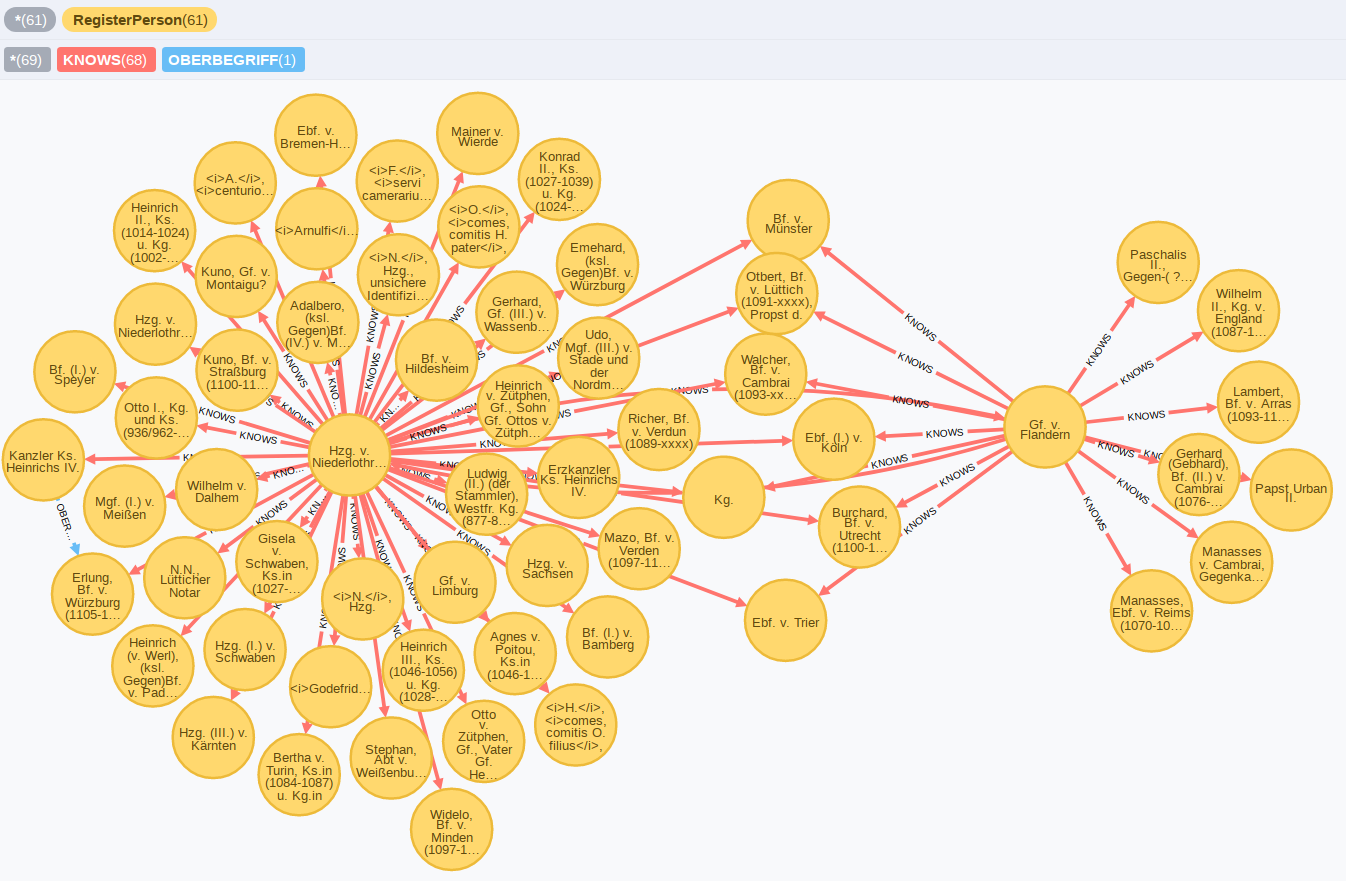
\includegraphics{Bilder/RI2Graph/RobertUndHeinrichApoc.png}
\caption{Robert und Heinrich mit den gemeinsamen Bekanntschaften.}
\label{robertundheinrichapoc}
\end{figure}

In Abb. \ref{robertundheinrichapoc} sind die zwei Ego-Netzwerke von Heinrich (links) und Robert (rechts) mit den dazwischen liegenden gemeinsamen Bekanntschaften dargestellt. Es zeigt sich, dass Heinrich stärker sowohl mit Geistlichen als auch Weltlichen vernetzt war, während Robert insgesamt weniger Kontakte aber mit einem Schwerpunkt in der Geistlichkeit hatte.

Für den Historiker ist aber vor allem interessant, was in den Regesten steht, die Robert und Heinrich über die Mittelsmänner verbinden. Hierfür wird der Cypher-Query angepasst und sowohl Personen als auch die Regestentexte ausgegeben.

\begin{verbatim}
// Liste der Regesten als Ergebnis
MATCH
(startPerson:IndexPerson)-[:PERSON_IN]->
(regest1:Regesta)<-[:PERSON_IN]-(middlePerson:IndexPerson)
-[:PERSON_IN]->(regest2:Regesta)
<-[:PERSON_IN]-(endPerson:IndexPerson)
WHERE startPerson.registerId in ['H4P00926']
AND endPerson.registerId in ['H4P01822']
RETURN DISTINCT startPerson.name1,
regest1.ident, regest1.text,
middlePerson.name1, regest2.ident,
regest2.text, endPerson.name1;
\end{verbatim}

In der folgenden Abbildung wird ein Ausschnitt der Ergebnistabelle gezeigt. In der ersten Spalte der Tabelle finden sich Robert, anschließend die Angaben zum Regest, mit dem er mit der mitteleren Person (middlePerson.name1) verknüpft ist. Dem folgen schließlich die Angaben zum Regest, mit den die mittlere Person mit Robert in der letzten Spalte verbunden ist. Die Tabelle in Abb. \ref{robertheinrichtabelle} bietet einen Überblick zur Überlieferungssituation aus der Perspektive der Regesta Imperii.

\begin{figure}
\centering
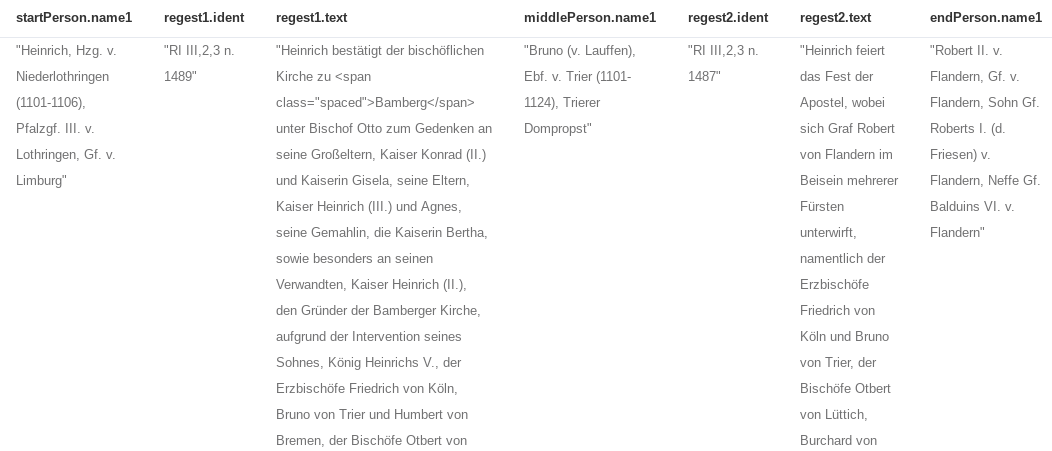
\includegraphics{Bilder/RI2Graph/RobertHeinrichApocTabelle.png}
\caption{Robert und Heinrich mit den gemeinsamen Bekanntschaften.}
\label{robertheinrichtabelle}
\end{figure}

\hypertarget{herrscherhandeln-ausgezuxe4hlt}{%
\subsection{Herrscherhandeln ausgezählt}\label{herrscherhandeln-ausgezuxe4hlt}}

Wie bereits oben erwähnt, wurde in einem ersten Test jeweils das erste Verb des Regestentextes extrahiert, lemmatisiert und in die Graphdatenbank eingespielt. Im folgenden werden nun einige Cypher-Querys vorgestellt, die dies beispielhaft auswerten.

\begin{verbatim}
// Herrscherhandeln ausgezählt
MATCH (n:Lemma)<-[h:ACTION]-(m:Regesta)
RETURN n.lemma, count(h) as ANZAHL ORDER BY ANZAHL desc LIMIT 10;
\end{verbatim}

\begin{longtable}[]{@{}ll@{}}
\toprule
n.lemma & ANZAHL\tabularnewline
\midrule
\endhead
werden & 145\tabularnewline
schenken & 133\tabularnewline
bestätigen & 109\tabularnewline
begehen & 95\tabularnewline
verleihen & 48\tabularnewline
ernennen & 36\tabularnewline
nehmen & 35\tabularnewline
treffen & 34\tabularnewline
empfangen & 29\tabularnewline
erhalten & 26\tabularnewline
\bottomrule
\end{longtable}

Die Ergebnisliste zeigt gleich die Einschränkungen, da das Hilfsverb \emph{werden} aus dem textuellen Zusammenhang gerissen ist. Andererseits ergeben sich aber auch interessante Erkenntnisse zur Häufigkeitsverteilung von Herrscherhandeln in Regestentexten. Die Anwendung des Verfahrens auf Regestentexte ist dabei auf der einen Seite positiv, da bei der Erstellung der Regesten sehr stark auf formale Kriterien geachtet wird und so die Zusammenhänge gut zu erfassen sind. Auf der anderen Seite ist die Auswertung aber wiederum einen weiteren Schritt von der ursprünglichen Quelle entfernt.

\hypertarget{herrscherhandeln-pro-ausstellungsort-ausgezuxe4hlt}{%
\subsection{Herrscherhandeln pro Ausstellungsort ausgezählt}\label{herrscherhandeln-pro-ausstellungsort-ausgezuxe4hlt}}

Im folgenden Query kommt eine räumliche Komponente zur Abfrage hinzu, da das Lemma hier jeweils abhängig vom Ausstellungsort der Urkunde abgefragt wird.

\begin{verbatim}
// Herrscherhandeln pro Ausstellungsort
MATCH (n:Lemma)<-[h:ACTION]-(:Regesta)-[:PLACE_OF_ISSUE]->(p:Place)
WHERE p.normalizedGerman IS NOT NULL
RETURN p.normalizedGerman, n.lemma, count(h) as ANZAHL ORDER BY ANZAHL desc LIMIT 10;
\end{verbatim}

\begin{longtable}[]{@{}lrr@{}}
\toprule
p.normalizedGerman & n.lemma & ANZAHL\tabularnewline
\midrule
\endhead
Mainz & begehen & 15\tabularnewline
Mainz & schenken & 14\tabularnewline
Goslar & schenken & 13\tabularnewline
Rom & werden & 12\tabularnewline
Regensburg & schenken & 12\tabularnewline
Goslar & begehen & 11\tabularnewline
Speyer & schenken & 10\tabularnewline
Worms & begehen & 8\tabularnewline
Regensburg & bestätigen & 7\tabularnewline
Regensburg & werden & 7\tabularnewline
\bottomrule
\end{longtable}

In der ersten Spalte befindet sich der Ortsname, der aus der Property \texttt{normalizedGerman} des \texttt{Place}-Knotens stammt. In der zweiten Spalte wird das Lemma angegeben und in der dritten Spalte schließlich die Anzahl der jeweiligen Regesten. Interessant wäre hier auch noch die Ergänzung der zeitlichen Dimension, mit der dann der zeitliche Verlauf in die Auswertung miteinbezogen werden könnte.

\hypertarget{herrscherhandeln-und-anwesenheit}{%
\subsection{Herrscherhandeln und Anwesenheit}\label{herrscherhandeln-und-anwesenheit}}

Im nächsten Beispiel werden in einem Regest genannten Personen in die Auswertung des Herrscherhandelns mit einbezogen.

\begin{verbatim}
MATCH (p:IndexPerson)-[:PERSON_IN]-(r:Regesta)-[:ACTION]-(l:Lemma)
RETURN p.name1, l.lemma, count(l) AS Anzahl ORDER BY p.name1, Anzahl DESC;
\end{verbatim}

\begin{longtable}[]{@{}lrr@{}}
\toprule
\begin{minipage}[b]{0.67\columnwidth}\raggedright
p.name1\strut
\end{minipage} & \begin{minipage}[b]{0.16\columnwidth}\raggedleft
l.lemma\strut
\end{minipage} & \begin{minipage}[b]{0.09\columnwidth}\raggedleft
Anzahl\strut
\end{minipage}\tabularnewline
\midrule
\endhead
\begin{minipage}[t]{0.67\columnwidth}\raggedright
\ldots{}\strut
\end{minipage} & \begin{minipage}[t]{0.16\columnwidth}\raggedleft
\ldots{}\strut
\end{minipage} & \begin{minipage}[t]{0.09\columnwidth}\raggedleft
\ldots{}\strut
\end{minipage}\tabularnewline
\begin{minipage}[t]{0.67\columnwidth}\raggedright
Adalbero, Metzer Domkanoniker, Kanzler Heinrichs IV., Kanzler (Gegen)Kg. Rudolfs v. Rheinfelden\strut
\end{minipage} & \begin{minipage}[t]{0.16\columnwidth}\raggedleft
schenken\strut
\end{minipage} & \begin{minipage}[t]{0.09\columnwidth}\raggedleft
21\strut
\end{minipage}\tabularnewline
\begin{minipage}[t]{0.67\columnwidth}\raggedright
Adalbero, Metzer Domkanoniker, Kanzler Heinrichs IV., Kanzler (Gegen)Kg. Rudolfs v. Rheinfelden\strut
\end{minipage} & \begin{minipage}[t]{0.16\columnwidth}\raggedleft
bestätigen\strut
\end{minipage} & \begin{minipage}[t]{0.09\columnwidth}\raggedleft
9\strut
\end{minipage}\tabularnewline
\begin{minipage}[t]{0.67\columnwidth}\raggedright
Adalbero, Metzer Domkanoniker, Kanzler Heinrichs IV., Kanzler (Gegen)Kg. Rudolfs v. Rheinfelden\strut
\end{minipage} & \begin{minipage}[t]{0.16\columnwidth}\raggedleft
verleihen\strut
\end{minipage} & \begin{minipage}[t]{0.09\columnwidth}\raggedleft
4\strut
\end{minipage}\tabularnewline
\begin{minipage}[t]{0.67\columnwidth}\raggedright
Adalbero, Metzer Domkanoniker, Kanzler Heinrichs IV., Kanzler (Gegen)Kg. Rudolfs v. Rheinfelden\strut
\end{minipage} & \begin{minipage}[t]{0.16\columnwidth}\raggedleft
erlassen\strut
\end{minipage} & \begin{minipage}[t]{0.09\columnwidth}\raggedleft
2\strut
\end{minipage}\tabularnewline
\begin{minipage}[t]{0.67\columnwidth}\raggedright
Adalbero, Metzer Domkanoniker, Kanzler Heinrichs IV., Kanzler (Gegen)Kg. Rudolfs v. Rheinfelden\strut
\end{minipage} & \begin{minipage}[t]{0.16\columnwidth}\raggedleft
übertragen\strut
\end{minipage} & \begin{minipage}[t]{0.09\columnwidth}\raggedleft
2\strut
\end{minipage}\tabularnewline
\begin{minipage}[t]{0.67\columnwidth}\raggedright
Adalbero, Metzer Domkanoniker, Kanzler Heinrichs IV., Kanzler (Gegen)Kg. Rudolfs v. Rheinfelden\strut
\end{minipage} & \begin{minipage}[t]{0.16\columnwidth}\raggedleft
ermäßigen\strut
\end{minipage} & \begin{minipage}[t]{0.09\columnwidth}\raggedleft
2\strut
\end{minipage}\tabularnewline
\begin{minipage}[t]{0.67\columnwidth}\raggedright
Adalbero, Metzer Domkanoniker, Kanzler Heinrichs IV., Kanzler (Gegen)Kg. Rudolfs v. Rheinfelden\strut
\end{minipage} & \begin{minipage}[t]{0.16\columnwidth}\raggedleft
gestatten\strut
\end{minipage} & \begin{minipage}[t]{0.09\columnwidth}\raggedleft
2\strut
\end{minipage}\tabularnewline
\begin{minipage}[t]{0.67\columnwidth}\raggedright
Adalbero, Metzer Domkanoniker, Kanzler Heinrichs IV., Kanzler (Gegen)Kg. Rudolfs v. Rheinfelden\strut
\end{minipage} & \begin{minipage}[t]{0.16\columnwidth}\raggedleft
vollziehen\strut
\end{minipage} & \begin{minipage}[t]{0.09\columnwidth}\raggedleft
1\strut
\end{minipage}\tabularnewline
\begin{minipage}[t]{0.67\columnwidth}\raggedright
Adalbero, Metzer Domkanoniker, Kanzler Heinrichs IV., Kanzler (Gegen)Kg. Rudolfs v. Rheinfelden\strut
\end{minipage} & \begin{minipage}[t]{0.16\columnwidth}\raggedleft
nehmen\strut
\end{minipage} & \begin{minipage}[t]{0.09\columnwidth}\raggedleft
1\strut
\end{minipage}\tabularnewline
\begin{minipage}[t]{0.67\columnwidth}\raggedright
Adalbero, Metzer Domkanoniker, Kanzler Heinrichs IV., Kanzler (Gegen)Kg. Rudolfs v. Rheinfelden\strut
\end{minipage} & \begin{minipage}[t]{0.16\columnwidth}\raggedleft
mindern\strut
\end{minipage} & \begin{minipage}[t]{0.09\columnwidth}\raggedleft
1\strut
\end{minipage}\tabularnewline
\begin{minipage}[t]{0.67\columnwidth}\raggedright
Adalbero, Metzer Domkanoniker, Kanzler Heinrichs IV., Kanzler (Gegen)Kg. Rudolfs v. Rheinfelden\strut
\end{minipage} & \begin{minipage}[t]{0.16\columnwidth}\raggedleft
setzen\strut
\end{minipage} & \begin{minipage}[t]{0.09\columnwidth}\raggedleft
1\strut
\end{minipage}\tabularnewline
\begin{minipage}[t]{0.67\columnwidth}\raggedright
\ldots{}\strut
\end{minipage} & \begin{minipage}[t]{0.16\columnwidth}\raggedleft
\ldots{}\strut
\end{minipage} & \begin{minipage}[t]{0.09\columnwidth}\raggedleft
\ldots{}\strut
\end{minipage}\tabularnewline
\bottomrule
\end{longtable}

Die Ergebnistabelle zeigt den Abschnitt zu Adalbero, einem Metzer Domkanoniker, mit der Häufigkeit des jeweiligen Herrscherhandeln-Lemmas.

\hypertarget{regesten-200-km-rund-um-augsburg}{%
\subsection{Regesten 200 km rund um Augsburg}\label{regesten-200-km-rund-um-augsburg}}

Mit dem folgenden Query werden für den Umkreis von 200 km rund um Augsburg alle Regesten aufgerufen.

\begin{verbatim}
// Entfernungen von Orten berechnen lassen
MATCH (n:Place)
WHERE n.normalizedGerman = 'Augsburg'
WITH n.latLong as point
MATCH (r:Regesta)
WHERE distance(r.latLong, point) < 200000
AND r.placeOfIssue IS NOT NULL
AND r.placeOfIssue <> 'Augsburg'
RETURN r.ident, r.placeOfIssue,
distance(r.latLong, point) AS Entfernung
ORDER BY Entfernung;
\end{verbatim}

Solche Queries lassen sich auch mit zeitlichen Abfragen kombinieren und bieten sehr flexible Abfragemöglichkeiten.

\hypertarget{welche-literatur-wird-am-meisten-zitiert}{%
\subsection{Welche Literatur wird am meisten zitiert}\label{welche-literatur-wird-am-meisten-zitiert}}

Beim Import der Regesten in die Graphdatenbank werden die mit dem RI-Opac verlinkten Literaturtitel als eigenständige \texttt{Reference}-Knoten angelegt und jeweils mit dem \texttt{Regesta}-Knoten verknüpft. Diese Verknüpfung wird mit dem folgenden Query abgefragt, ausgezählt und aufgelistet.

\begin{verbatim}
MATCH (n:Reference)<-[r:REFERENCES]-(m:Regesta)
RETURN n.title, count(r) AS Anzahl
ORDER BY Anzahl DESC LIMIT 10;
\end{verbatim}

\begin{longtable}[]{@{}lr@{}}
\toprule
n.title & ANZAHL\tabularnewline
\midrule
\endhead
Stumpf & 215\tabularnewline
Böhmer & 201\tabularnewline
Ldl & 101\tabularnewline
Jaffé & 60\tabularnewline
Schmale & 56\tabularnewline
Buchholz & 51\tabularnewline
Scheffer-Boichorst & 50\tabularnewline
Wauters & 39\tabularnewline
Dobenecker & 33\tabularnewline
Remling & 28\tabularnewline
\bottomrule
\end{longtable}

Mit diesen Daten lassen sich Zitationsnetzwerke in den Regesten darstellen mit denen Regesten gefunden werden können, die auf Grund der gemeinsam zitierten Literatur die gleichen inhaltlichen Schwerpunkte aufweisen können.

\hypertarget{der-import-zusammengefasst}{%
\subsection{Der Import zusammengefasst}\label{der-import-zusammengefasst}}

Den komplette \href{cypher/20_cypher-Datenbankerstellung.txt}{Cypher-Code} für die Erstellung der Graphdatenbank ist zusammengefasst über eine \href{cypher/20_cypher-Datenbankerstellung.txt}{Textdatei} abrufbar. Es ist zu empfehlen, die aktuelle Version von neo4j-Desktop zu installieren, eine Graphdatenbank anzulegen und in der Graphdatenbank die Apoc-Bibliothek zu installieren. Inzwischen ist es möglich, in der Befehlszeile des neo4j-Browsers auch mehrere Befehle nacheinander ausführen zu lassen. Alternativ kann nach dem Start der Graphdatenbank im Reiter \texttt{Terminal} mit dem Befehl \texttt{bin/cypher-shell} die cypher-shell aufgerufen werden. In diese Shell werden dann alle Befehl gemeinsam hineinkopiert und ausgeführt. Alternativ zur Installation von neo4j kann auch auf den Internetseiten von neo4j eine \href{https://neo4j.com/lp/try-neo4j-sandbox}{Sandbox} erstellt werden.

\hypertarget{zusammenfassung-2}{%
\section{Zusammenfassung}\label{zusammenfassung-2}}

In diesem Kapitel wurden die Schritte zum Import der Regesten Kaiser Heinrichs IV. in die Graphdatenbank neo4j erläutert sowie verschiedene Auswertungsbeispiele vorgestellt.

\hypertarget{verwandtschaft-im-graphen}{%
\chapter{Verwandtschaft im Graphen}\label{verwandtschaft-im-graphen}}

In diesem Kapitel wird am Beispiel eines Ausschnitts der Daten des Projekts \textbf{Nomen et Gens}\footnote{Informationen zum Projekt „Nomen et Gens`` finden Sie unter \url{http://www.neg.uni-tuebingen.de/} (abgerufen am 10.08.2018).} die Modellierung von Verwandtschaft in der Graphdatenbank neo4j dargestellt.\footnote{Dieses Kapitel geht in großen Teilen zurück auf meinem Aufsatz Graphentechnologien in den Digitalen Geisteswissenschaften, in: ABI Technik 2017; 37(3): 179--196, \url{https://doi.org/10.1515/abitech-2017-0042}. URL: \url{https://www.degruyter.com/downloadpdf/j/abitech.2017.37.issue-3/abitech-2017-0042/abitech-2017-0042.pdf}, insbesondere die Seiten 179 bis 182 und wurde nur geringfügig ergänzt. Herrn Prof.~Dr.~Steffen Patzold danke ich herzlich für die Erlaubnis, die Nomen et Gens Daten im Rahmen dieser Publikation zu verwenden (mit Mail vom 22.01.2019).}

\hypertarget{das-projekt-nomen-et-gens}{%
\section{Das Projekt Nomen et Gens}\label{das-projekt-nomen-et-gens}}

Das Projekt \textbf{Nomen et Gens} (NeG) zielt darauf ab, alle schriftlich belegten Namen und Personen Kontinentaleuropas in den vier Jahrhunderten vor Karl dem Großen (also von 400 bis 800 nach Christus) zu erfassen. Die Datenbank des Projekts geht auf ein erfolgreich abgeschlossenes DFG-Projekt zurück und wird aktuell von den Projektbeteiligten weiter betreut und sukzessive ausgebaut. Neben den Quellen der Personennennung, den unterschiedlichen Namensformen usw. werden auch die Verwandtschaftsbeziehungen zwischen identifizierten Personen in der Datenbank abgelegt. Dabei werden bis zu 16 verschiedene Verwandtschaftsbeziehungen in der Datenbank gespeichert, wie z. B. Bruder, Schwester, Sohn, Tochter, Vater, Mutter, Onkel oder Nichte. Bei einem Personendatensatz werden dann jeweils die Verwandtschaftsbeziehungen aufgelistet, so dass man sich ggf. jeweils von Person zu Person durchklicken muss, bis man am Ziel angelangt ist.

\hypertarget{nomen-et-gens-im-graphen}{%
\section{Nomen et Gens im Graphen}\label{nomen-et-gens-im-graphen}}

Vor diesem Hintergrund bot es sich an, die Personen und die zugehörigen Verwandtschaftsbeziehungen in die Graphdatenbank neo4j zu transferieren und anschließend graphbasierte Abfrageperspektiven zu testen.

\begin{figure}
\centering
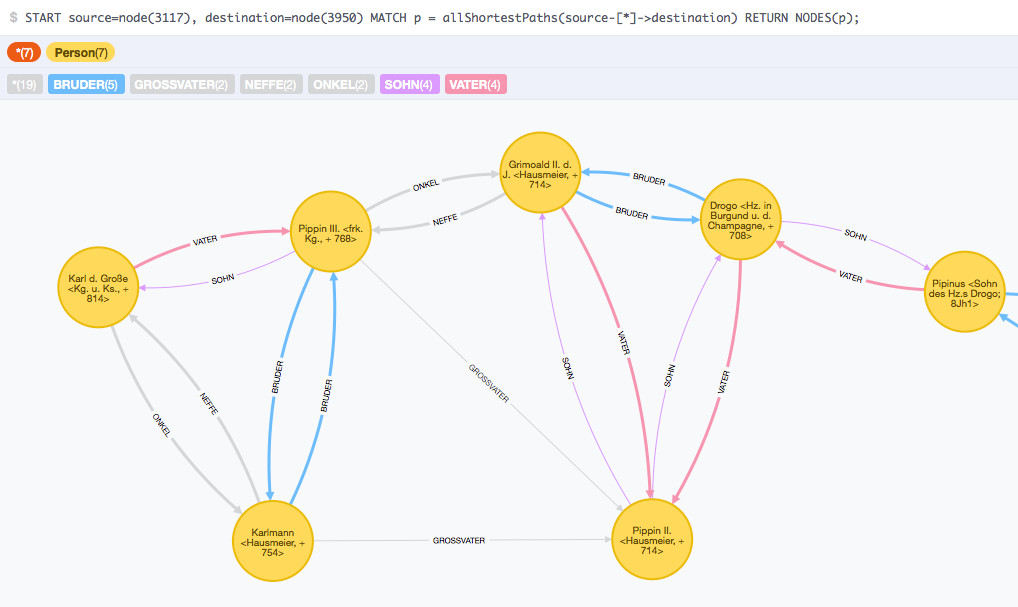
\includegraphics{Bilder/NeG/020-Verwandschaften.jpg}
\caption{Erste Importergebnisse}
\label{importergebnisse}
\end{figure}

Abb. \ref{importergebnisse} zeigt die ersten Ergebnisse des Datenbankimports. Aus der Visualisierung werden die zahlreichen redundanten Beziehungen deutlich, die in der Folge zu neuen Modellierungsansätzen für die Verwandtschaftsbeziehungen führten. Ergebnis der Überlegungen war die Reduzierung der möglichen Verwandtschaftsbeziehungen auf die zwei Kantentypen \texttt{KIND} und \texttt{VERHEIRATET\_MIT}. Dabei wird eine Kante vom Typ \texttt{KIND} für eine Elternteil-Kind-Beziehung nur einmal vergeben, während eine Kante vom Typ \texttt{VERHEIRATET\_MIT} immer zweifach in jeweils umgekehrter Richtung angelegt wird. Dies ergibt sich aus der Überlegung, dass eine Elternteil-Kind-Beziehung gerichtet ist und zwar in unserem Fall vom Elternteil zum Kind hin, während eine \texttt{VERHEIRATET\_MIT}-Beziehung ungerichtet ist: Wenn eine Person mit einer anderen Person verheiratet ist, ist die andere Personen automatisch auch mit der ersten verheiratet. Da im Property-Graph-Modell von neo4j jede Kante genau eine Richtung haben muss, wird die \texttt{VERHEIRATET\_MIT}-Kante zweimal in jeweils unterschiedliche Richtung angelegt, während bei der hierarchischen Elternteil-Kind-Beziehung eine Kante ausreicht (vgl. Abb \ref{urenkel}).

\begin{figure}
\centering
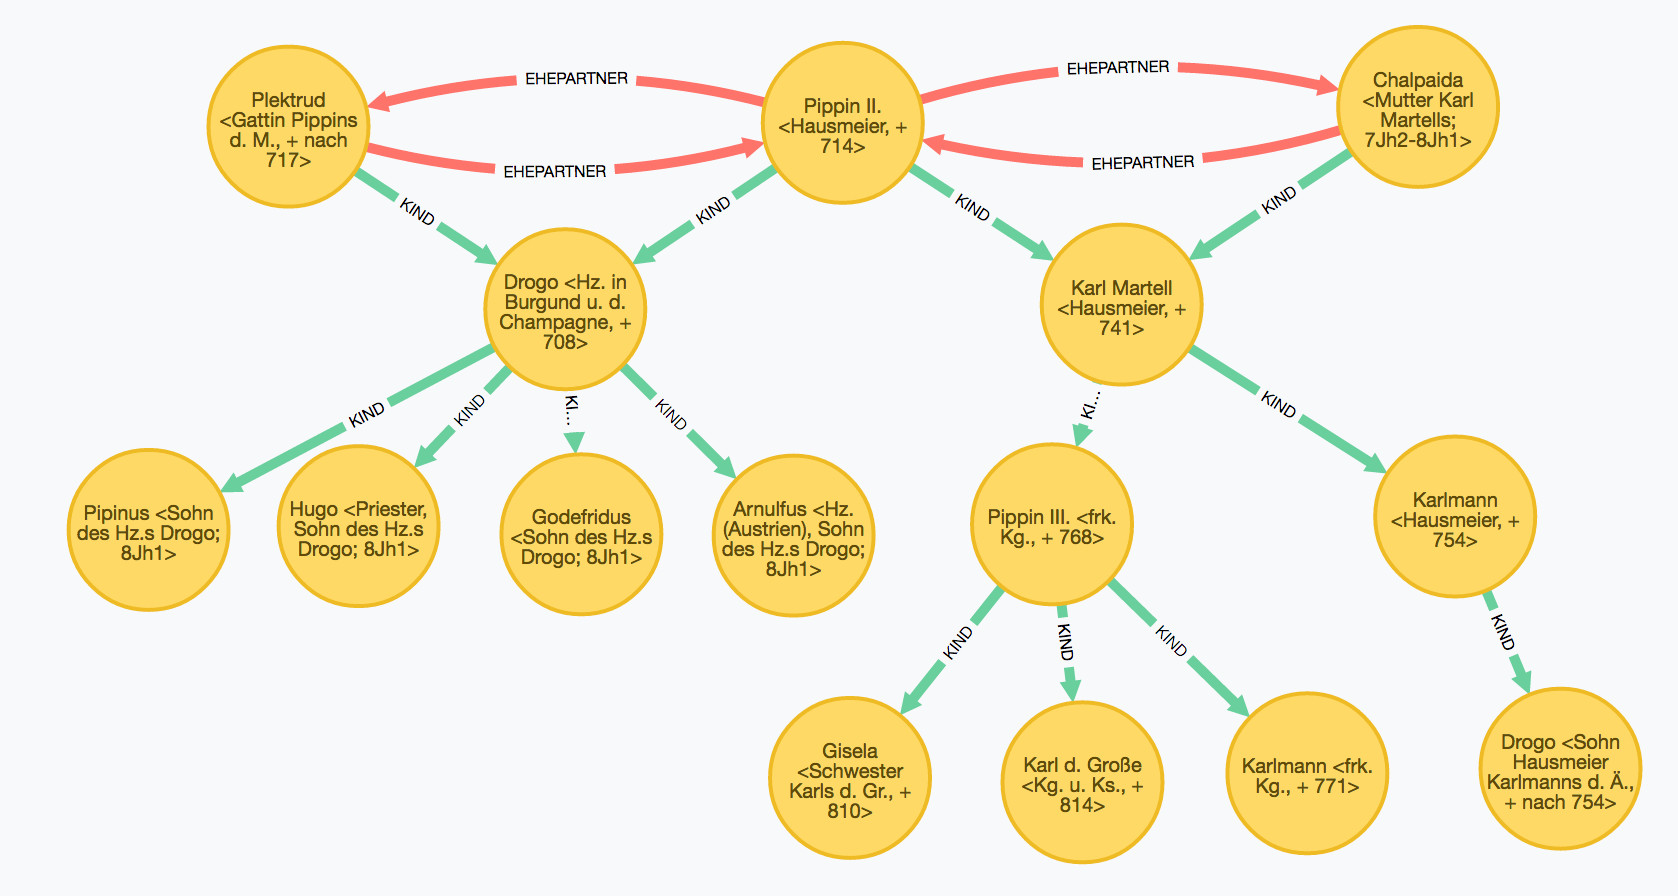
\includegraphics{Bilder/NeG/030-Urenkel-Pippins.jpg}
\caption{Die Urenkel Pippins}
\label{urenkel}
\end{figure}

\hypertarget{sind-berchar-und-karl-der-grouxdfe-verwandt}{%
\section{Sind Berchar und Karl der Große verwandt ?}\label{sind-berchar-und-karl-der-grouxdfe-verwandt}}

Im folgenden Beispiel soll das Potential der Graphmodellierung von Verwandtschaftsbeziehungen demonstriert werden. In der Datenbank gibt es die Person Berchar (Abb. \ref{berchar}). Berchar war ein Hausmeier König Theuderichs III. Die Frage ist nun, ob dieser Berchar mit Karl dem Großen verwandt ist. In der NeG-Datenbank ist ein Verwandtschaftsverhältnis von Berchar zu Karl dem Großen nicht direkt ableitbar.

\begin{figure}
\centering
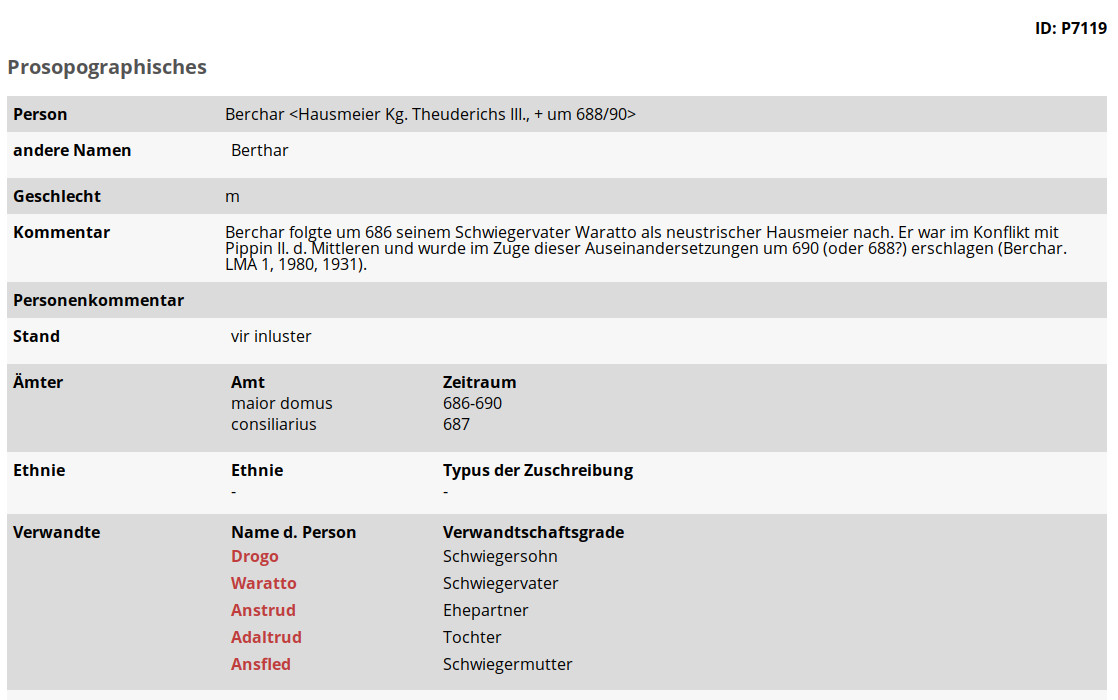
\includegraphics{Bilder/NeG/040-Berchar-DB-Eintrag.jpg}
\caption{Berchar in der Nomen-et-Gens-Datenbank}
\label{berchar}
\end{figure}

In der Graphdatenbank neo4j wird für eine solche Fragestellung eine Shortest\_Path-Abfrage verwendet, die den kürzesten möglichen Weg zwischen zwei Knoten zurück liefert, sofern es einen gibt. Der folgende Cypher-Befehl liefert den Pfad zwischen dem Personenknoten Karls des Großen mit der NeG-ID \texttt{7404} und dem Personenknoten von Berchar mit der NeG-ID \texttt{7119}. Dabei wird die Länge des abzufragenden Pfades auf 15 Kanten begrenzt.

\begin{verbatim}
// shortest_path-Abfrage von Karl dem Großen zu Berchar
MATCH (KdG:Person { nid:'7404' })
MATCH (Berchar:Person { nid:'7119' })
p = shortestPath((KdG)-[*..15]-(Berchar))
RETURN p;
\end{verbatim}

Das Ergebnis (Abb. \ref{shortestpath}) zeigt, dass Berchar tatsächlich mit Karl dem Großen verwandt ist. Er ist nämlich der Schwiegervater von Drogo (Herzog in Burgund und der Champagne, gest. 708), der wiederum der Bruder des Großvaters Karls des Großen ist.

\begin{figure}
\centering
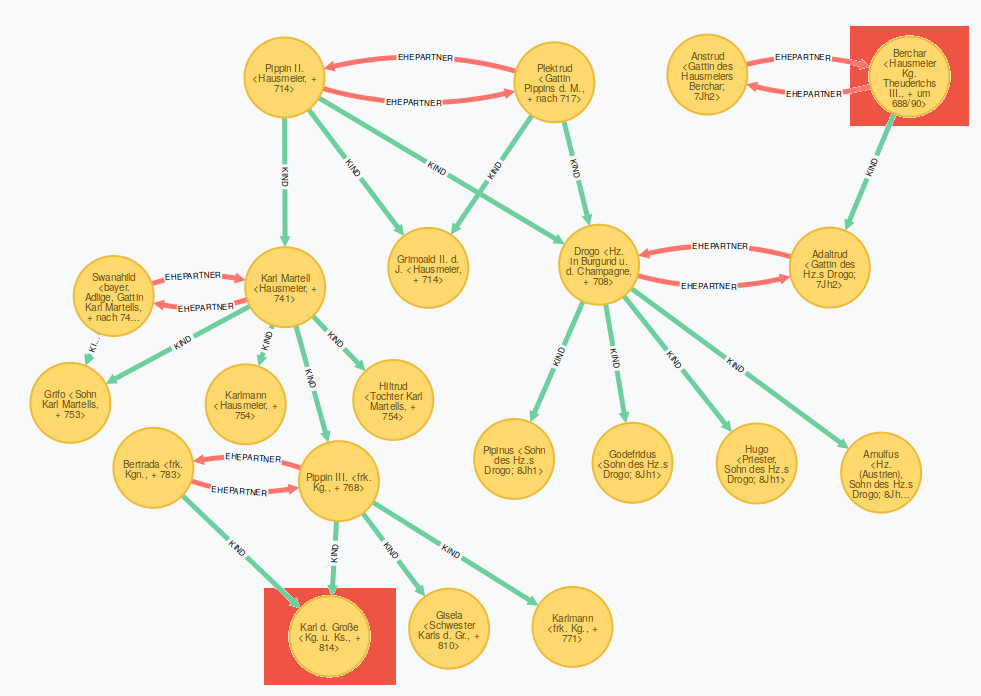
\includegraphics{Bilder/NeG/050-Berchar-Karl-shortestpath.jpg}
\caption{Der kürzeste Pfad (shortestPath) von Karl zu Berchar.}
\label{shortestpath}
\end{figure}

\hypertarget{zusammenfassung-3}{%
\section{Zusammenfassung}\label{zusammenfassung-3}}

Mit diesem Beispiel sind die interessanten Erschließungs- und Modellierungsperspektiven für die digitale Genealogie nur angedeutet. Mit Graphentechnologien lässt sich intuitive Datenmodellierung mit sehr flexiblen Erschließungs- und Abfragemöglichkeiten kombinieren.

\hypertarget{zusammenfassung-4}{%
\chapter{Zusammenfassung}\label{zusammenfassung-4}}

Anhand der verschiedenen Beispiele konnte gezeigt werden, dass Graphentechnologien hervorragend für die Modellierung, Speicherung und Analyse hochvernetzter Daten geeignet sind. Ebenso konnten die Beispiele zeigen, dass die digitalen Geisteswissenschaften reich an hochvernetzten Daten sind. Gleichzeitig lassen sich mit dem einer Mind-Map sehr ähnlichen Modell Forschungsdaten und Forschungsfragestellungen tatsächlich in einer Weise modellieren, die dem menschlichen Denken sehr nahe kommt. Damit können Graphentechnologien gleichsam als Brücke zwischen den geisteswissenschaftlichen Fachdisziplinen und den informationstechnologischen Herausforderungen und Perspektiven des digitalen Zeitalters dienen.

So gelingt es in den digitalen Geisteswissenschaften mit dem Graphenmodell bei der Modellierung und Strukturierung von Forschungsdaten und Forschungsfragestellungen die Kluft zwischen Informatiker und Geisteswissenschaftler zu schließen, da der Graph eine für beide Seiten verständliche Plattform bietet. Für den Informatiker ist er hinreichend genau und berechenbar und für den Geisteswissenschafter wegen seiner Schema- und Hierarchiefreiheit ausreichend flexibel. Gerade diese Eigenschaften, mit denen sich die beiden zentralen Zweige der Digitalen Geisteswissenschaften vereinen lassen, machen Graphen zu einem Schlüsselkonzept der Geisteswissenschaften des 21. Jahrhunderts.

\end{document}
